\documentclass[12pt,]{book}
\usepackage{lmodern}
\usepackage{amssymb,amsmath}
\usepackage{ifxetex,ifluatex}
\usepackage{fixltx2e} % provides \textsubscript
\ifnum 0\ifxetex 1\fi\ifluatex 1\fi=0 % if pdftex
  \usepackage[T1]{fontenc}
  \usepackage[utf8]{inputenc}
\else % if luatex or xelatex
  \ifxetex
    \usepackage{mathspec}
  \else
    \usepackage{fontspec}
  \fi
  \defaultfontfeatures{Ligatures=TeX,Scale=MatchLowercase}
\fi
% use upquote if available, for straight quotes in verbatim environments
\IfFileExists{upquote.sty}{\usepackage{upquote}}{}
% use microtype if available
\IfFileExists{microtype.sty}{%
\usepackage{microtype}
\UseMicrotypeSet[protrusion]{basicmath} % disable protrusion for tt fonts
}{}
\usepackage[margin=1in]{geometry}
\usepackage{hyperref}
\hypersetup{unicode=true,
            pdftitle={Challenges and Tools in the Assessment and Management of Pacific Salmon Fisheries},
            pdfauthor={Ben Staton},
            pdfborder={0 0 0},
            breaklinks=true}
\urlstyle{same}  % don't use monospace font for urls
\usepackage{natbib}
\bibliographystyle{apalike}
\usepackage{longtable,booktabs}
\usepackage{graphicx,grffile}
\makeatletter
\def\maxwidth{\ifdim\Gin@nat@width>\linewidth\linewidth\else\Gin@nat@width\fi}
\def\maxheight{\ifdim\Gin@nat@height>\textheight\textheight\else\Gin@nat@height\fi}
\makeatother
% Scale images if necessary, so that they will not overflow the page
% margins by default, and it is still possible to overwrite the defaults
% using explicit options in \includegraphics[width, height, ...]{}
\setkeys{Gin}{width=\maxwidth,height=\maxheight,keepaspectratio}
\IfFileExists{parskip.sty}{%
\usepackage{parskip}
}{% else
\setlength{\parindent}{0pt}
\setlength{\parskip}{6pt plus 2pt minus 1pt}
}
\setlength{\emergencystretch}{3em}  % prevent overfull lines
\providecommand{\tightlist}{%
  \setlength{\itemsep}{0pt}\setlength{\parskip}{0pt}}
\setcounter{secnumdepth}{5}
% Redefines (sub)paragraphs to behave more like sections
\ifx\paragraph\undefined\else
\let\oldparagraph\paragraph
\renewcommand{\paragraph}[1]{\oldparagraph{#1}\mbox{}}
\fi
\ifx\subparagraph\undefined\else
\let\oldsubparagraph\subparagraph
\renewcommand{\subparagraph}[1]{\oldsubparagraph{#1}\mbox{}}
\fi

%%% Use protect on footnotes to avoid problems with footnotes in titles
\let\rmarkdownfootnote\footnote%
\def\footnote{\protect\rmarkdownfootnote}

%%% Change title format to be more compact
\usepackage{titling}

% Create subtitle command for use in maketitle
\newcommand{\subtitle}[1]{
  \posttitle{
    \begin{center}\large#1\end{center}
    }
}

\setlength{\droptitle}{-2em}

  \title{Challenges and Tools in the Assessment and Management of Pacific Salmon
Fisheries}
    \pretitle{\vspace{\droptitle}\centering\huge}
  \posttitle{\par}
    \author{Ben Staton}
    \preauthor{\centering\large\emph}
  \postauthor{\par}
    \date{}
    \predate{}\postdate{}
  
\usepackage{booktabs}
%%% This is an example file for the Auburn University style options
%%%       aums.sty (Masters Thesis)
%%%       auphd.sty (Ph.D. Dissertation)
%%%       auhonors.sty (Honors Scholar)

%%%To use it, please edit the necessary options, title, author, date, year, keywords, advisor, professor, etc. 

% \documentclass[12pt]{report}
\usepackage{setspace}
% \usepackage{titlesec}
%\setcounter{secnumdepth}{3}
% \usepackage{aums}       % For Master's papers
\usepackage{auphd}     % For Ph.D.
%\usepackage{auhonors}  % For honors college
\usepackage[normalem]{ulem}       % underlining on style-page; see \normalem below
\usepackage{url}
\usepackage[table]{xcolor}
\usepackage{tikz}
\usepackage{pgf}
\usepackage{color,soul}

\usepackage{amsmath,amsthm, amsfonts, mathrsfs, graphicx, setspace, fullpage, color}
\usepackage{natbib, appendix}
\usepackage[T1]{fontenc}
\usepackage{multirow}
\usepackage{mathabx}
\RequirePackage{adjustbox}
% \usepackage{epstopdf}
\AtBeginDocument{\renewcommand{\bibname}{References}}
\usepackage{hyperref}
%\usepackage{tocloft}
%\renewcommand\cftchapafterpnum{\vskip\baselineskip}
%\renewcommand\cftsecafterpnum{\vskip\baselineskip}
%\renewcommand\cftsubsecafterpnum{\vskip\baselineskip}
%\renewcommand\cftsubsubsecafterpnum{\vskip\baselineskip}
%\renewcommand\cftfigafterpnum{\vskip\baselineskip}
%\renewcommand\cfttabafterpnum{\vskip\baselineskip}

% remove double spacing from itemized lists
\usepackage{enumitem}
% \setlist[itemize]{noitemsep}
\setlist{before=\singlespacing,after=\singlespacing}


%%%%%Format rules: Normal margins are 1 in. If you need to print with 1.5in margins, uncomment the line below
%\oddsidemargin0.5in \textwidth6in

%% If you do not need a List of Abbreviations, then comment out the lines below and the \printnomenclature line.
%%for List of Abbreviations information:  (see http://www.mackichan.com/TECHTALK/509.htm  )
% \usepackage[intoc]{nomencl}
% \renewcommand{\nomname}{List of Abbreviations}   	       
% \makenomenclature 
%% don't forget to run:   makeindex ausample.nlo -s nomencl.ist -o ausample.nls
%% Also, if 

\makeatother
\let\oldmaketitle\maketitle
\AtBeginDocument{\let\maketitle\relax}

% Put the title, author, and date in. 
\title{Challenges and Tools in the Assessment and Management of Pacific Salmon Fisheries}
\author{Benjamin A. Staton} 
\date{May 5, 2019} %date of graduation
\copyrightyear{2019} %copyright year

\keywords{Fisheries management, Bayesian inference, decision analysis}

% Put the Thesis Adviser here. 
\adviser{Matthew J. Catalano}

% Put the committee here (including the adviser), one \professor for each. 
% The advisor must be first, and the dean of the graduate school must be last.
\professor{Matthew J. Catalano, AFFILIATION}

\professor{Asheber Abebe, AFFILIATION}

\professor{Lewis G. Coggins, Jr., AFFILIATION}

\professor{Conor P. McGowan, AFFILIATION}
\usepackage{booktabs}
\usepackage{longtable}
\usepackage{array}
\usepackage{multirow}
\usepackage[table]{xcolor}
\usepackage{wrapfig}
\usepackage{float}
\usepackage{colortbl}
\usepackage{pdflscape}
\usepackage{tabu}
\usepackage{threeparttable}
\usepackage{threeparttablex}
\usepackage[normalem]{ulem}
\usepackage{makecell}

\usepackage{amsthm}
\newtheorem{theorem}{Theorem}[chapter]
\newtheorem{lemma}{Lemma}[chapter]
\theoremstyle{definition}
\newtheorem{definition}{Definition}[chapter]
\newtheorem{corollary}{Corollary}[chapter]
\newtheorem{proposition}{Proposition}[chapter]
\theoremstyle{definition}
\newtheorem{example}{Example}[chapter]
\theoremstyle{definition}
\newtheorem{exercise}{Exercise}[chapter]
\theoremstyle{remark}
\newtheorem*{remark}{Remark}
\newtheorem*{solution}{Solution}
\begin{document}
\maketitle

\begin{romanpages}      % roman-numbered pages 

\TitlePage 

\doublespacing
\setlength{\parskip}{0pt plus 0pt minus 0pt}

\begin{abstract} 
\noindent
I'm going to write an abstract to go here. This is the first paragraph of the dissertation abstract, which will talk about chapter 1..

This is the second paragraph of the dissertation abstract, which will talk broadly about chapter 2.

This is the third paragraph of the dissertation abstract, which will talk broadly about chapter 3.

This is the fourth paragraph of the dissertation abstract, which will talk broadly about chapter 4.
\end{abstract}

\begin{acknowledgments}
\noindent
Here is where I will thank everyone.

Matt, Lew, Brendan, Mike, Sam, AL-HPC folks, Steve, Nick, Zach, Janessa. Family and Michelle. Folks at the lab. RStudio staff.
\end{acknowledgments}

\begin{singlespace}
	\tableofcontents
	\clearpage
	\listoffigures
	\clearpage
	\listoftables
\end{singlespace}

% \printnomenclature[0.5in] %used for the List of Abbreviations
\end{romanpages}        % All done with roman-numbered pages

\normalem       % Make italics the default for \em

% \titlespacing\section{0pt}{12pt plus 4pt minus 2pt}{0pt plus 2pt minus 2pt}
% \titlespacing\subsection{0pt}{12pt plus 4pt minus 2pt}{0pt plus 2pt minus 2pt}
% \titlespacing\subsubsection{0pt}{12pt plus 4pt minus 2pt}{0pt plus 2pt minus 2pt}

\setlength{\parskip}{0pt plus 0pt minus 0pt}

\doublespacing

\chapter*{Preface}\label{preface}
\addcontentsline{toc}{chapter}{Preface}

I used bookdown \citep{xie-2015} to make this document.

\chapter{Introduction}\label{ch1}

\noindent
Pacific salmon (\emph{Oncorhynchus} spp.) constitute an integral natural
resource in Alaska to subsistence, commercial, and recreational
interests. There is a long history of resource development,
exploitation, regulation, and dependence on these resources within the
region \citep{cooley-1963}. In many cases, the resource use is dictated
by the locality of the system; for example, stocks located near urban
areas are often primarily exploited by recreational fishers whereas more
remote stocks often constitute commercial and/or subsistence uses. This
proposed dissertation focuses on the challenges and solutions in the
assessment and management of these more remote stocks and the
subsistence fisheries that rely heavily upon them.

Wild Pacific salmon represent a fantastic natural resource, which
results largely from their unique life history strategy. Pacific salmon
exhibit a migratory strategy known as anadromy: they spawn in freshwater
where eggs hatch and juveniles rear for several years. Juveniles then
migrate to the ocean where they spend the majority of their lives
feeding on abundant prey resources. Once reaching maturity, adults
return to their natal streams to spawn and complete the life cycle. The
result of this life history strategy is an incredibly productive
resource that grows entirely on its own and delivers itself to
harvesters when the time comes for exploitation.

Like for all exploited natural resources, the management of Pacific
salmon fisheries involves making decisions about how to exploit the
resource in order to best attain a suite of biological, social, and
economic objectives \citep{walters-1986}. These decisions are
intrinsically difficult due to conflicting objectives and uncertainties
in system state, system response to management actions, and
implementation \citep{walters-holling-1990}. Put another way, assuming a
manager knows exactly what they wish to obtain, getting there is made
difficult by not knowing how large the harvestable surplus is, how the
stock will respond to harvesting, or that their management action will
actually obtain what is desired. Despite these difficulties, a decision
must be made \citep[without decision-making there is no
management;][]{hilborn-walters-1992} and the consequences, whether
favorable or undesirable, must be accepted. Thus, I would argue that the
science of monitoring, assessment, and prediction in the context of
Pacific salmon fisheries is tasked with identifying trade-offs and
reducing uncertainty, both of which insert difficulty into the
decision-making process as discussed below.

The management of Pacific salmon fisheries can be thought of as a
hierarchy of (1) guiding objectives, (2) management strategies to attain
objectives, and (3) tactics to implement the management strategies
(Table \ref{tab:mgmt-hierarchy-table}). At the upper level, long-term
decisions are made about the objectives of the resource exploitation.
These long-term objectives constitute what could be referred to as
fundamental objectives: they are desired endpoints, but do not at all
imply how they should be attained. These fundamental objectives often
involve notions of sustainability and maintenance of biological
diversity and often include social objectives such as maximization and
stability of harvest. Already, it is clear that these fundamental
objectives are often conflicting. For example, consider the objective of
maximizing harvest: in fisheries that harvest multiple stocks (i.e.,
distinct spawning units), oftentimes maximum harvest may only obtained
by overexploiting weak stock components and possibly reducing diversity.
As another example, consider the objective of long-term sustainability:
in order to ensure that the stock is sustained, some level of harvest
fluctuations must be accepted (lower harvests must be allowed when the
stock is at low abundance). These conflicting objectives imply that
trade-offs exist (all objectives cannot be maximized simultaneously). It
is worth noting here that the decisions made at the uppermost level of
the management hierarchy are purely social and economic and salmon stock
assessment scientists should play little-to-no advisory or advocacy
roles in making these decisions \citep{walters-martell-2004}. The Policy
for the Management of Sustainable Salmon Fisheries (5 AAC 39.222) states
that the objectives of salmon management in Alaska are

\begin{quote}
``\ldots{}to ensure conservation of salmon and salmon's required marine
and aquatic habitats, protection of customary and traditional
subsistence uses and other uses, and the sustained economic health of
Alaska's fishing communities''.
\end{quote}

\noindent
The policy goes on to say that managers should target ``\ldots{} to the
extent possible, maximum sustained yield {[}MSY{]}''.

The second level of the management hierarchy is made up of harvest
strategies and policies that guide how the long term objectives are to
be obtained. The State of Alaska has selected the fixed escapement
policy as the management strategy to obtain the long-term objectives of
sustainability and yields that are close to the maximum. These
escapement goals are given as ranges that dictate the target number of
spawning adults each year; any portion of the stock above the escapement
goal is considered surplus (excess biological production) and should be
harvested. Uncertainty at this intermediate level of the management
hierarchy (i.e., regarding the optimal escapement goal) is often a
result of incomplete understanding of system status and function. For
example, in order to determine what the optimal escapement goal should
be to obtain MSY, knowledge of stock productivity and carrying capacity
are required. These quantities are often derived using spawner-recruit
analyses, which are inherently uncertain: data are rarely informative
about the shape of the true underlying spawner-recruit relationship but
instead provide a probabilistic distribution of expected outcomes at a
given stock size \citep{walters-martell-2004}. Traditionally, it has
been thought that these uncertainties can be reduced by more monitoring
and the development of rigorous assessment and prediction models to
better understand system function. However, it has often been argued
that while monitoring and assessment models are obviously important
(performance relative to objectives must be measured), true
understanding of system behavior comes only from experimentation in
management \citep[the concept of ``active adaptive
management'';][]{walters-1986}. The classic example is to assess the
maximum productivity of the stock (i.e., in the absence of density
dependent mortality), the spawning stock must be forced to small sizes
and the resulting recruitments must be observed. However, management
actions that ensure these observations are made are undesirable to many
managers and stakeholders, considering that exploiting a stock down to
these low levels is risky \citep{walters-1986}.

At the lower level in the management hierarchy, intra-annual (or
in-season) decisions are made regarding how to exploit the current
year's run to attain the long-term objectives. In other words, given a
management strategy (i.e., fixed escapement), the manager is still
tasked with deciding how to best implement the fishery within a year to
ensure the strategy is followed. As will be illustrated in this proposed
dissertation, these decisions at the intra-annual level of the
management hierarchy are often poorly informed by data which often
results in indecisiveness, subjectivity, non-transparency, frustration,
and missed opportunities.

This proposed dissertation will be partitioned into three chapters, each
that expands on and investigates the performance of potential solutions
to the aforementioned difficulties in Pacific management in Western
Alaska. Each chapter will focus on the Kuskokwim River drainage in
Western Alaska, which is characterized by being a large drainage
(\textgreater{}50,000 km\textsuperscript{2}), harvests are taken by
primarily subsistence users who are nearly all native Alaskans, and the
primary species of interest being Chinook salmon. Although this proposed
dissertation is quite narrow in its geographical and biological focus, a
wide range of management issues will be addressed and the developed
tools and assessment methods will be evaluated thoroughly. Furthermore,
the concepts and tools discussed, developed, and evaluated will be
generalizable to other stocks with similar spatial structures,
exploitation characteristics, and population dynamics.

Chapter \ref{ch2} will work at the intra-annual level of the hierarchy
to develop and evaluate the performance of a run timing forecast model
that can be used to aid in the interpretation of in-season data. As will
be shown, uncertainty in run timing makes the interpretation of
in-season data incredibly difficult. For example, consider a case in
which an abundance index has produced high counts early in the season
when compared to the historical average. This observation is consistent
with at least two run scenarios: (1) a small run with early run timing
or (2) a large run with average timing. There is a large discrepancy in
the amount of harvestable surplus suggested by each of these discrete
scenarios, leading to a large amount of uncertainty about how the
fishery should be executed. The overall objective of Chapter \ref{ch2}
will be to develop and evaluate the reliability of a run timing forecast
model for Kuskokwim River Chinook salmon. A secondary goal of Chapter
\ref{ch2} will be to formally assess the utility of having access to the
run timing forecast model in terms of reducing uncertainty and bias in
run size indices used in intra-annual management decisions.

Chapter \ref{ch3} will again address the lowest level of the management
hierarchy (i.e., intra-annual decision-making), but in this case in a
more direct sense using an analysis framework known broadly as
Management Strategy Evaluation (MSE). This analysis will seek to
evaluate several harvest control tactics to identify strategies that
perform well at attaining pre-defined objectives (e.g., meeting the
escapement goal, distributing harvest equally across villages and stock
components, etc.) across a range of biological states (e.g., run size,
stock composition, and run timing). This analysis is needed because
while the fixed escapement strategy seems simple to execute, actually
doing so is made difficult largely due to uncertainty regarding the size
of the incoming run (i.e., the amount of harvestable surplus is not
known). Additionally, there may be a set of tactics that perform well at
limiting harvest in low run size years but doing so in a ``fair way',
where the burdens of shortages aren't carried primarily by a certain
subset of resource users. If a consistent set of rules or triggers could
be identified that perform reasonably well at meeting management
objectives without precise knowledge of run size, it could prove very
useful to managers and decision making within the region.

Chapter \ref{ch4} will move up the hierarchy to the second level and
will seek to extend the single stock assessment models currently used in
many systems in Alaska to multi-stock assessments. When an aggregate
stock is made up of several distinct components, each with their own
productivity, it is likely that exploitation at some level (e.g., 50\%)
results in the more productive components being under-exploited while
the weaker stocks may be over-exploited. This reality implies a
trade-off: to preserve stock diversity, some harvest must be foregone.
Before the shape and magnitude of these types of
``harvest-biodiversity'' trade-offs are quantified, some understanding
of the variation in substock productivity and carrying capacity is
required. The multi-stock assessment framework developed in Chapter
\ref{ch4} will be tailored to provide this information for these sorts
of trade-off analyses and others that require similar information
sources. Multi-stock assessments may assume one of several different
model structures (e.g., by fitting separate models to the data from each
stock or by fitting a single model to all data simultaneously). In some
cases, one approach may be preferable over the other, and a primary
objective of Chapter \ref{ch4} will be to evaluate the performance of a
range of assessment strategies (in terms of accuracy and precision)
across a range of biological and data quality conditions.

\newpage

\begin{table}

\caption{\label{tab:mgmt-hierarchy-table}One way of viewing the structure of renewable natural resource (including salmon) management as described in the text, including examples of alternatives and sources of uncertainty at each level.}
\centering
\begin{tabular}[t]{ll}
\toprule
\textbf{Examples} & \textbf{Sources of Uncertainty}\\
\midrule
\addlinespace[0.3em]
\multicolumn{2}{l}{\textbf{Overarching Objectives}}\\
\hline
\hspace{1em}Ensure sustainability & Relative importance of objectives\\
\hspace{1em}Maximize harvest & Problem boundaries\\
\hspace{1em}Stabilize harvest & \\
\hspace{1em}Maximize economic value & \\
\addlinespace[0.3em]
\multicolumn{2}{l}{\textbf{Inter-annual Strategies}}\\
\hline
\hspace{1em}Constant escapement & Stock productivity\\
\hspace{1em}Constant exploitation rate & Stock status\\
\hspace{1em}Constant catch & Drivers of stock change\\
\hspace{1em}Adaptive exploitation & Shape/magnitude of trade-offs\\
\addlinespace[0.3em]
\multicolumn{2}{l}{\textbf{Intra-annual Tactics}}\\
\hline
\hspace{1em}Triggers and thresholds & Harvestable surplus\\
\hspace{1em}Time, area, gear restrictions & Uninformative data\\
\hspace{1em}Limited participation & Fisher behavior\\
\bottomrule
\end{tabular}
\end{table}

\chapter{Development and Evaluation of a Migration Timing Forecast Model
for Kuskokwim River Chinook Salmon}\label{ch2}

\section*{Abstract}\label{abstract}
\addcontentsline{toc}{section}{Abstract}

Annual variation in adult salmon migration timing makes the
interpretation of in-season assessment data difficult, leading to much
in-season uncertainty in run size. We developed and evaluated a run
timing forecast model for the Kuskokwim River Chinook salmon stock,
located in western Alaska, intended to aid in reducing this source of
uncertainty. An objective and adaptive approach (using model-averaging
and a sliding window algorithm to select predictive time periods, both
calibrated annually) was adopted to deal with multidimensional selection
of four climatic variables and was based entirely on predictive
performance. Forecast cross-validation was used to evaluate the
performance of three forecasting approaches: the null (i.e., intercept
only) model, the single model with the lowest mean absolute error, and a
model-averaged forecast across 16 nested linear models. As of 2018, the
null model had the lowest mean absolute error (2.64 days), although the
model-averaged forecast performed as well or better than the null model
in the majority of retrospective years. The model-averaged forecast had
a consistent mean absolute error regardless of the type of year (i.e.,
average or extreme early/late) the forecast was made for, which was not
true of the null model. The availability of the run timing forecast was
not found to increase overall accuracy of in-season run assessments in
relation to the null model, but was found to substantially increase the
precision of these assessments, particularly early in the season.

\section{Introduction}\label{introduction}

\noindent
In-season management strategies for Pacific salmon (\emph{Oncorhynchus}
spp.) fisheries rely heavily on indices of in-river abundance (e.g.,
test fisheries, sonar counts, etc.) to inform harvest control rules that
attempt to attain the balance of meeting pre-determined escapement
objectives while allowing adequate opportunity for harvest
\citep{catalano-jones-2014}. However, because indices of abundance are
confounded by the phenology (i.e., timing) of the migration, their
interpretation is very difficult in-season. For example,
smaller-than-average index values early in the season could be due to
either a small run with average timing or by a late large run, when
interpreted in the context of historical years
\citep{adkison-cunningham-2015}. This ultimately leads to great
uncertainty about how much of the incoming run has passed, which is a
key piece of information that dictates fishery harvest opportunities.
There exists no information in the current year's abundance index to
inform the manager if (for example) 25\% or 75\% of the run has passed
on any given day. Yet, depending which is true, the optimal management
decision could be vastly different. Thus, in-season assessment typically
involves some characterization of the variation in historical run timing
to formulate a range of possible run size scenarios that could be
representative of the current year's run size. However, given the amount
of variation in historical run timing, these scenarios are rarely
informative during the majority of the migration, when key harvest
decisions are being made because the run scenarios may span all possible
run sizes. As a result, the pre-season run size forecast remains the
most precise piece of information for much of the season. If it were
possible to predict the timing of the incoming run (e.g., earlier- or
later-than-average) with some level of confidence, it could prove
valuable for in-season assessment and decision-making by reducing
uncertainty in run size predictions.

While previous research has uncovered several key physiological
mechanisms that are involved with natal homing
\citep{hasler-scholz-1983} and return migrations of adult salmon to
freshwater environments
\citep{cooperman-etal-2010, cooke-etal-2008, hinch-etal-2012}, the exact
physiological and behavioral responses of adult salmon to relatively
small-scale environmental gradients within estuaries, which are likely
the ultimate determinants of freshwater entry timing, are still poorly
understood. Despite this uncertainty, several hypotheses have been put
forth that are broadly consistent with the observed timing patterns of
several species across a large geographic area (i.e., western and
southwestern Alaska). Two primary influences have been suggested:
genetic \citep{quinn-etal-2000, anderson-beer-2009, omalley-etal-2010}
and environmental \citep{hodgson-etal-2006, keefer-etal-2008}
mechanisms. Substantial evidence exists to suggest that both genetic and
environmental controls are involved in determining migration timing,
however it is broadly thought that genetic variation influences
sub-stock variation (i.e., different tributary spawning groups within
the same major river basin) and environmental variation influences the
timing of the aggregate (i.e., basin-wide) run
\citep{keefer-etal-2008, anderson-beer-2009}. This is consistent with
the notion that genetically distinct components of the aggregate run
behave differently as a result of their life history strategies and/or
the characteristics of their specific spawning grounds
\citetext{\citealp[e.g., sub-stocks that must travel farther in-river to
reach spawning grounds enter freshwater
earlier;][]{clark-etal-2015}; \citealp[sub-stocks that spawn in
tributaries influenced by warmer lakes enable later
spawning;][]{burger-etal-1985}} but that certain environmental
conditions act on the aggregate run to either hasten or delay freshwater
entry. It has also been suggested that run size may have an influence on
migration timing, although empirical support for this claim seems to be
lacking. If there were indeed relationships between run timing and run
size, these need to be quantified as certain combinations are
particularly troublesome for managers \citep[e.g., small/early runs and
large/late runs appear the same early
in-season;][]{adkison-cunningham-2015}.

At the aggregate population scale, which is the focus of this Chapter,
it has been observed that migrations occurring in the spring and summer
generally occur earlier in years with warmer spring temperatures
{[}\citet{mundy-evenson-2011}; hodgson-etal-2006{]}.
\citet{mundy-evenson-2011} suggested that this pattern may be explained
by the stability of the estuarine water column where adult salmon stage
in preparation for riverine entry (or alternatively, marine exit). High
estuarine water column stability was hypothesized to impede riverine
entry through two mechanisms:

\begin{enumerate}
\def\labelenumi{(\arabic{enumi})}
\tightlist
\item
  by presenting an osmotic barrier between freshwater riverine discharge
  and the saline ocean water which prevents osmotically incompetent
  individuals from crossing and,
\item
  by preventing freshwater competent individuals from receiving
  olfactory cues essential to the homeward migration.
\end{enumerate}

\noindent
Thus, \citet{mundy-evenson-2011} hypothesized that years in which the
estuarine water column is stable over a longer period of time would be
associated with later migration timing. Although water column stability
is a difficult variable to measure over large spatial scales, several
variables that are known to influence it are available at large scales
via remote sensing (e.g., satellite observations). Such variables are
sea ice cover which prevents wind-driven mixing, associated local
temperature-related variables like land-based air temperature or sea
surface temperature (SST), and broader scale indicators such as the
Pacific Decadal Oscillation (PDO), an index of temperature anomalies in
the northern Pacific Ocean. Observational studies across the North
American range of Chinook salmon have found environmental-run timing
correlations that are consistent with this hypothesis
\citep{hodgson-etal-2006, keefer-etal-2008, mundy-evenson-2011}. Even if
the water column stability hypothesis is incorrect, observed patterns
suggest that environmental variables may be useful in forecasting run
timing with some level of accuracy and certainty.

Several efforts have been made at exploiting these environmental-run
timing relationships to develop run timing forecast models for Pacific
salmon migrations. \citet{mundy-evenson-2011} developed a model for
Yukon River Chinook salmon (\emph{O. tshawytscha}) that used air
temperature, SST, and ice cover to predict the day at which the
\(15^{\text{th}}\) and \(50^{\text{th}}\) percentiles of the run passed
a test fishery index location. Their model predictions fit the observed
data well (nearly always within seven days, usually within three days),
although out-of-sample predictive ability was not presented.
\citet{keefer-etal-2008} developed a similar framework for Columbia
River spring run Chinook salmon and found run timing relationships with
river discharge, river temperature, and ocean condition indices (e.g.,
PDO). Their best model explained 49\% of the variation in median run
timing with variation in the environmental variables.
\citet{anderson-beer-2009} continued this work on the Columbia River
spring Chinook stock, but added genetic components to their analysis
based on the arrival timing of precocious males. Their findings revealed
that both environmental variables and changes in abundance of
genetically distinct populations, which had their own distinct migration
timing and affected overall run timing of the spring Chinook salmon run
in the Columbia River. These advancements have shown that relationships
between migration timing and environmental variables exist and may have
utility for use in forecasting efforts.

The Kuskokwim River, located in western Alaska, is the second largest
river system in the state and supports culturally and economically
important Chinook salmon fisheries. Chinook salmon return beginning in
late May and continue through early August, with the median date of
passage occurring between June 14 and July 2. Fisheries within the
region harvest salmon in-river during freshwater migrations using
primarily drift gillnet gear. The Kuskokwim River salmon fishery has a
distinct cultural importance: nearly all inhabitants are native Alaskans
belonging to the Yup'ik group and take salmon for subsistence purposes
\citep{linderman-bergstrom-2009}. While commercial salmon fisheries
operate within the river, these fishers often also participate in
subsistence take and revenues from the sale of commercially-harvested
salmon often contribute directly to participation in subsistence
activities \citep{wolfe-spaeder-2009}. To ensure long-term sustainable
harvest, the Chinook salmon fishery is managed with a drainage-wide
escapement goal derived from an age-structured state-space
spawner-recruit analysis \citep{hamazaki-etal-2012, staton-etal-2017a}.
To meet these pre-determined escapement goals, in-season management
strategies implement time, gear, and area closures based on limited and
imprecise information regarding annual run size. The distant locations
of the majority of escapement assessment projects makes direct
measurement of escapement performance unavailable until late in the
season. Thus, the primary sources of run size assessment information are
(1) a pre-season run size forecast range (obtained as the previous
year's run size estimate \(\pm \sim 20\%\)) and (2) an in-river drift
gillnet test fishery operated in Bethel, AK which has been implemented
using consistent methods since 1984. The interpretation of this test
fishery index suffers from the same issue of being confounded by run
timing described earlier, making management decisions difficult. Without
precise in-season indicators of run size, managers must often choose to
either trust a pre-season run size forecast for the majority of the
season or somehow place weights on the various run timing hypotheses
when interpreting in-season data. Both options could lead to the wrong
interpretation of the actual run size, which could have serious
consequences for the management of the fishery in a given year (i.e.,
the unwarranted opening or closing the fishery resulting in severe
under- or over-escapement). No published run timing forecast models
currently exist for Kuskokwim River Chinook salmon but given the
potential utility of independent run timing estimates for interpretation
of in-season data, the development and evaluation of such a model is
needed. The necessity of more accurate and precise in-season perceptions
of run size is particularly evident in years with anticipated low runs,
such as in recent years (i.e., since 2010), as this may allow managers
to more effectively guard against over-exploitation while still allowing
for limited harvest opportunities to support the cultural and
subsistence needs of the region.

In this chapter, I present an analysis that develops and evaluates the
performance of a run timing forecast model for Kuskokwim River Chinook
salmon. The objectives were to

\begin{enumerate}
\def\labelenumi{(\arabic{enumi})}
\tightlist
\item
  quantify historical run timing,
\item
  develop a run timing forecast model using environmental variables
  selected based on out-of-sample predictive performance
\item
  assess the utility of the forecasting model for improving predictions
  of end-of-season test fishery indices of run size,
\item
  determine if there is a relationship between run size and run timing
  for the Kuskokwim River Chinook salmon stock.
\end{enumerate}

\section{Methods}\label{methods}

\subsection{Estimates of migration
timing}\label{estimates-of-migration-timing}

\noindent
In this analysis, the forecasted quantity that represented migration
timing was the day at which 50\% of the run passed an index location
(hereafter, \(D_{50}\)). To inform this quantity for each year in the
analysis, we used daily catch-per-unit-effort (CPUE) data from the
Bethel Test Fishery (BTF) operated by the Alaska Department of Fish and
Game (ADF\&G), which spans 1984 -- 2018. The raw data were daily CPUE
beginning on June 1 and ending August 24 each year. The cumulative sum
of these daily CPUE values within a year follows a sigmoidal pattern
reflecting the shape of the incoming salmon run which is characterized
by relatively few early migrants, a peak where the majority of the fish
are running, and relatively few late migrants. To estimate the median
day of passage as a continuous variable, a logistic model was fitted to
the cumulative proportion of daily CPUE of the form:

\begin{equation}
  p_{d,t}=\frac{1}{1 + e^{-h_t (d - D_{50,t})}},
  \label{eq:logistic}
\end{equation}

\noindent
where \(p_{d,t}\) is the predicted cumulative proportion on
day-of-the-year (DOY) \(d\) in calendar year \(t\), \(h_t\) is the
parameter that controls the steepness of the curve (i.e., duration of
the run), and \(D_{50,t}\) is the day at which 50\% of the total annual
CPUE was caught in year \(t\). Annual estimates of \(D_{50,t}\) and
\(h_t\) were obtained by fitting \(p_{d,t}\) to observed daily
cumulative proportion by minimizing the sum of squared deviations from
the model prediction. Uncertainty in these parameter estimates was not
further considered in the analysis as the uncertainty was negligible.
Further, the use of the BTF daily CPUE values to infer the location and
shape of year-specific logistic timing curves made the assumption that
these data provided an accurate representation of daily run strength
within a year (i.e., that the influence of weather conditions or harvest
on sampling was negligible).

\subsection{Environmental variables}\label{environmental-variables}

\noindent
Environmental variables to be assessed for forecasting performance were
chosen based on three criteria:

\begin{enumerate}
\def\labelenumi{(\arabic{enumi})}
\tightlist
\item
  previously established association with salmon run timing,
\item
  availability for the Kuskokwim River during the years for which BTF
  index observations exist (1984 -- 2018), and
\item
  availability for use in a pre-season forecast model (i.e., available
  no later than June 10\textsuperscript{th} in the year for which the
  forecasted value would be used).
\end{enumerate}

\noindent
Based on these criteria, four environmental variables were chosen for
analysis: SST, percent sea ice cover (SIC), PDO, and land-based air
temperature taken in Bethel, AK.

\subsubsection{PDO data}\label{pdo-data}

\noindent
Data collected for the PDO variable came from one of several indices
produced by the National Oceanic and Atmospheric Administration (NOAA)
\citep{mantua-etal-1997}\footnote{PDO data:
  \url{http://research.jisao.washington.edu/pdo/PDO.latest.txt}}. The
index is produced by taking the first principal component of monthly SST
anomalies in the northern Pacific Ocean, after removing any global
trends due to any systematic change over time \citep{mantua-etal-1997}.
Thus, for each year of the data set, a single monthly value was
available for PDO. Previous studies have found PDO values prior to the
initiation of the run have predictive value for Chinook salmon
populations \citep{beer-2007, keefer-etal-2008}.

\subsubsection{Bethel air temperature
data}\label{bethel-air-temperature-data}

\noindent
Air temperature data for Bethel, AK were accessed from the Alaska
Climate Research Center\footnote{Alaska air temperature data:
  \url{http://akclimate.org/acis_data}}. These data were available as
daily means for each day of each year in the 1984 -- 2018 data set.

\subsubsection{SST and SIC}\label{sst-and-sic}

\noindent
SST and SIC data were accessed from the NOAA Optimum Interpolation SST
V2 High Resolution Dataset \citep{reynolds-etal-2007}\footnote{Global
  gridded SST and SIC:
  \url{http://www.esrl.noaa.gov/psd/data/gridded/data.noaa.oisst.v2.highres.html}}.
These data were available as daily means for any 0.25° by 0.25° latitude
by longitude grid cell on the globe. To limit the search, only grid
cells within Kuskokwim Bay were selected for analysis Figure
\ref{fig:ch2-map} as that is the area that Chinook salmon bound for the
Kuskokwim River likely aggregate prior to riverine entry. The area with
grid cells ranged from 58.5° N to 60° N by 164.25° W to 162° W, which
resulted in a total of 54 0.25° latitude by 0.25° longitude grid cells.
For SST, four grid cells fell partially over land (resulting in 50 grid
cells with daily data) and for SIC, five grid cells were partially over
land (49 grid cells with daily data). ``Empty'' grid cells were excluded
and the remaining grid cells were used for prediction. Previous analyses
have used a simple average over a wide spatial area
\citep[e.g.,][]{mundy-evenson-2011} to create a single value for SST or
SIC each year. However, this is somewhat arbitrary and does not account
for the possibility of certain areas having stronger timing signals than
others or that the areas with stronger signals may change over time.
Thus, the gridded spatial structure of these variables was retained and
the treatment of this structure in the forecast analysis is discussed
below in Section \ref{rtf-models}.

\subsection{Forecast model}\label{reg-models}

To produce a forecast of run timing, relationships between historical
observed pairs of the environmental variables each year and \(D_{50,t}\)
must be quantified. The simple linear regression framework was used to
obtain these historical relationships:

\begin{equation}
  \begin{split}
    D_{50,t} = \beta_0 + \beta_j x_{t,j} +,...,+ \beta_n x_{t,J} + \varepsilon_t, \\
    \varepsilon_t \stackrel{\text{iid}}{\sim} N(0, \sigma) \\
  \end{split}
\label{eq:lin-reg}
\end{equation}

\noindent
where \(D_{50,t}\) is the observed run timing value in year \(t\),
\(x_{t,j}\) is the observed value of covariate \(j\) (of which there are
\(J\) included in the model), \(\beta_0\) and \(\beta_j\) are
coefficients linking the observed values of \(D_{50,t}\) with
\(x_{t,j}\), \(\varepsilon_t\) are random residual effects that explain
deviations of observed \(D_{50,t}\) from the fitted value and have
constant variance equal to \(\sigma^2\).

There are many such regression models that could be used to produce a
run timing forecast (i.e., \(\hat{D}_{50,t+1}\)). This is because:

\begin{enumerate}
\def\labelenumi{(\arabic{enumi})}
\tightlist
\item
  there are four variables (PDO, air temperature, SST, and SIC) that
  could be included,
\item
  each variable is temporally structured, i.e., there are daily or
  monthly values for each variable, and
\item
  two variables (SST and SIC) are spatially-explicit, i.e., there are
  different values for each day and year for different areas of
  Kuskokwim Bay (Figure \ref{fig:ch2-map}).
\end{enumerate}

\noindent
Item (1) deals with the specific values of \(j\) and \(J\) whereas items
(2) and (3) deal with what values of \(x_{t}\) for a given \(j\) should
take on.

\subsection{Selection of predictive time periods}\label{clim-windows}

\noindent
To fit the regression model in Equation \eqref{eq:lin-reg}, a single value
for each \(x_{t,j}\) was required. The covariate data were temporally
structured, however, indicating that some selection of which time
periods to use to populate \(x_{t,j}\) was required. Oftentimes the
average over an arbitrary time period, such as daily values in the month
of February, is used based on \emph{a priori} assumptions of the
behavior of important factors \citep{vandepol-etal-2016}. While this
approach is simple to implement and explain, it is possible that a
better time window (i.e., reliably more accurate) exists but was not
considered. Furthermore, the importance of various time windows may
change over time and the arbitrary selection of a single window does not
allow for such changes to be detected. To avoid these issues, a rigorous
temporal selection process, known as the sliding climate window
algorithm \citep[SCWA;][]{vandepol-etal-2016}, was implemented to
determine the best predictive time period for each variable considered
in the forecast model. To find the most reliable temporal window for
prediction, the SCWA evaluates all possible windows (subject to certain
restrictions) over which to average for use as the predictor variable in
the forecast model. The following section provides the details of the
SCWA.

\subsubsection{The SCWA}\label{the-scwa}

\noindent
A ``window'' in this context is hereafter defined as a block of
consecutive days in some portion of the year with starting
day-of-the-year (DOY) denoted by \(D_F\) and ending day equal to
\(D_L\). The daily values within each evaluated window were averaged for
the \(x_{t,j}\) value to be used in a linear regression framework. As
input constraints, the SCWA used in this analysis required:

\begin{enumerate}
\def\labelenumi{(\arabic{enumi})}
\tightlist
\item
  the start date of the first window to be evaluated (\(D_0\)),
\item
  the end date of the last window to be evaluated (\(D_n\)), and
\item
  the minimum window size of a candidate window (\(\Delta_{D,min}\)).
\end{enumerate}

\noindent
The algorithm started with the earliest and smallest possible time
window: \(D_F = D_0 = 1\) through
\(D_L = D_0 + \Delta_{D,min} - 1 = 5\). The performance of this window
when used to obtain \(x_{t,j}\) was evaluated (see Section \ref{fcst-cv}
below) and the result was stored for comparison to other candidate
windows. For the next window, \(D_F\) would remain at \(D_0\), but
\(D_L\) would be incremented by 1 day (\(\ell=1\)). Thus, the endpoints
of all candidate windows with \(D_F = D_0\) can be generalized as:

\begin{equation}
  [D_0, D_0 + \Delta_{D,min} - 1 + \ell],
\label{eq:scwa-1}
\end{equation}

\noindent
for each \(\ell = 0, 1, ..., n - 1\), where \(n = D_L - D_F + 1\). For
all windows, including those with \(D_F = D_0\), this generalizes to:

\begin{equation}
  [D_0 + f, D_0 + f + \Delta_{D,min} - 1 + \ell],
\label{eq:scwa-2}
\end{equation}

\noindent
for each \(f = 0, 1, ..., n - \Delta_{D,min}\) and
\(\ell = 0, 1, ..., n - \Delta_{D,min} - f\). Windows with
\(f > n - \Delta_{D,min}\) would contain fewer than \(\Delta_{D,min}\)
days and are thus prohibited. After evaluating all windows, the single
window with the best predictive performance was used to obtain the
forecast predictor variable for that data source (i.e., PDO
\emph{versus} air temperature). As an example, consider the following
inputs:

\begin{itemize}
\tightlist
\item
  \(D_0 = 1\) (i.e., the first day of the year),
\item
  \(D_n = 31\) (i.e., January 31), and
\item
  \(\Delta_{D,min}\) = 5.
\end{itemize}

The SCWA would start with January 1 - January 5, then do January 1-6,
January 1-7, etc., January 1-31. Next, it would exclude January 1 from
consideration and evaluate all windows starting with January 2. When it
completes the one window starting with January 27, it must stop because
windows starting later than January 27 would result in windows shorter
than 5 days. Example R code for how the sliding window algorithm was
implemented is provided in Appendix \protect\hyperlink{appendix-a}{A}.

The values of \(D_0\) and \(D_L\) for the four covariates are shown in
Table \ref{tab:scwa-dates-table}. For air temperature, SST, and SIC
\(\Delta_{D,min}\) was set to 5. Note that because PDO was available in
monthly values only, each month was treated as ``day'' in the algorithm
described above and \(\Delta_{D,min}\) was set to 1.

\subsubsection{Forecast cross-validation}\label{fcst-cv}

A metric was needed to measure the performance of the many windows. This
metric was obtained using a time series forecast cross-validation
procedure, which is an out-of-sample technique for data that are
collected through time \citep{arlot-celisse-2010}. The procedure
operated by producing a forecasted value of \(D_{50}\) for year \(t+1\)
trained based on all data \(x_{t,j}\) available from years
\(1, ..., t\). It then continued for all \(t = m, ..., n-1\), where
\(m\) is the minimum number of years necessary to fit the model (set at
\(m = 10\) in all cases) and \(n\) is the number of years of available
data. Then, absolute forecast error in was calculated based on all
forecasted years as \(|D_{50,t+1} - \hat{D}_{50,t+1}|\), and yearly
forecast errors were averaged to obtain mean absolute error
(\(\overline{\text{AE}}\)) which was used as the measure of model
performance in window selection. The window with the lowest
(\(\overline{\text{AE}}\)) was selected as the optimal window to average
over for prediction. The forecasting cross-validation procedure was used
as opposed to other out-of-sample validation procedures, such as
\(k\)-fold or leave-one-out methods, because the data were collected
through time and the forecast model would never need to predict (for
example) year 2010 from years 1984 -- 2009 and 2011 -- 2018, but rather
it would always need to predict year \(t+1\) from all
previously-collected data. Example R code for how the forecast
cross-validation was conducted is provided in Appendix
\protect\hyperlink{appendix-a}{A}.

When forecasting \(D_{50,t+1}\) from training data from \(1,...,t\), a
single optimal climate window was selected for each variable and that
window was used to estimate coefficients based on training data and
obtain the environmental variable value for prediction in year \(t+1\)
to forecast \(D_{50,t+1}\). When a new year of data was added to the
training data (such as in the retrospective forecast analysis; Section
\ref{retro}), the optimal window for each variable was re-assessed using
the algorithm again. For PDO and Bethel air temperature, which had no
spatial structure, the SCWA was used to select the range of monthly
(PDO) or daily (Bethel air temperature) values to include in the
predictive climate window for each year in the analysis. For SST and SIC
which contained a series of 50 and 49 grid cells, respectively, each
with unique daily values, the SCWA was used on each grid cell
separately. The result was 50 unique grid cell-specific windows for SST
and 49 windows for SIC for each year of the analysis. The treatment of
this spatial structure in the forecast analysis is discussed below in
Section \ref{rtf-models}.

\subsection{Evaluated forecast models}\label{rtf-models}

\noindent
Linear regression {[}Equation \eqref{eq:lin-reg}{]} was used to assess the
forecast performance of each of the variables described above, both in
isolation of and in combination with other variables. All possible
subsets were evaluated (excluding interactive effects) for predictive
ability through time, resulting in a total of 16 models ranging from the
null (i.e., intercept only) model to the full (i.e., global) model (all
four variables as additive predictors).

For the spatially-explicit variables (i.e., SST and SIC), a more complex
treatment was required to prevent all grid cell values from being used
as predictors in a single model. To handle the spatial structure, grid
cell-specific regression models were fitted, then model-averaging based
on AIC was used to obtain a single forecast \(D_{50}\) for each year
\citep{burnham-anderson-2002}. Under this approach, each grid cell \(g\)
received an AIC\textsubscript{c} score:

\begin{equation}
  \text{AIC}_{c,g}=n \log{\left(\hat{\sigma}_g^2\right) + 2K + \frac{2K(K+1)}{n-K-1}},
  \label{eq:aicc}
\end{equation}

\noindent
where \(n\) is the number of data points used in each model,
\(\hat{\sigma}_g\) is the estimate of the residual standard deviation
under grid \(g\), and \(K\) is the number of model parameters. The
corrected version of AIC (AIC\textsubscript{c}) is recommended in cases
where the ratio of \(n\) to \(K\) is small (Burnham and Anderson, 2002).
Then, each grid cell received a \(\Delta\text{AIC}_\text{c}\) score,
representing its relative performance in comparison to the best grid
cell:

\begin{equation}
  \Delta_g=\text{AIC}_{\text{c},g}-\text{AIC}_{\text{c},min},
  \label{eq:delta-aicc}
\end{equation}

\noindent
where \(\text{AIC}_{\text{c},min}\) is the minimum AIC\textsubscript{c}
across all grid cells. Model (grid cell) weights were then calculated
as:

\begin{equation}
  w_g=\frac{e^{-0.5\Delta_g}}{\sum_j^G e^{-0.5\Delta_j}},
\label{eq:aicc-weights}
\end{equation}

\noindent
where \(G\) is the number of grid cells. Grid cell-averaged predictions
were then obtained as:

\begin{equation}
  \hat{y}_{t+1}=\sum_g^G w_g \hat{y}_{g,t+1},
\label{eq:grid-avg-fcst}
\end{equation}

\noindent
where \(\hat{y}_{g,t+1}\) is the forecasted value of \(D_{50}\) for grid
cell \(g\).

\subsection{Forecast uncertainty}\label{forecast-uncertainty}

\noindent
In addition to forecast accuracy, forecast precision is also of great
importance. For models that did not require AIC\textsubscript{c}
model-averaging across grid cells, the following equation was used to
produce a forecast standard error (SE):

\begin{equation}
  \text{SE}=\hat{\sigma} \sqrt{1 + \frac{1}{n} + \frac{(x-\bar{x})^2}{\sum_i^n(x_i-\bar{x})^2}},
\label{eq:se}
\end{equation}

\noindent
where \(n\) is the number of years the model was fitted to, \(x\) is the
value of the predictor variable used for forecasting, and \(\bar{x}\) is
the mean of all predictor values excluding the new value used for
forecasting. For models that used AIC\textsubscript{c} model-averaging
(i.e., those including SST and SIC), the following equation was used to
produce prediction SE:

\begin{equation}
  \text{SE}=\sum_g^G w_g \sqrt{\text{SE}_g^2+(\hat{y}_{g,t+1}-\hat{y}_{t+1})^2},
\label{eq:mod-avg-se}
\end{equation}

\noindent
where \(\text{SE}_g\) is the prediction SE from grid cell \(g\)
calculated using equation \eqref{eq:se}. This estimator of unconditional
sampling standard error accounts for uncertainty within each model and
the uncertainty due to model selection \citep{burnham-anderson-2002}.
Prediction intervals were calculated using the point estimate of
prediction, the prediction SE, and appropriate quantiles from the
corresponding \(t\) distribution.

\subsection{Forecast model selection}\label{model-selection}

\noindent
Given 16 forecast models, it is impossible to know which will perform
the best at forecasting for the current year. Thus, three methods to
obtain a forecast for \(D_{50}\) were evaluated:

\begin{enumerate}
\def\labelenumi{(\arabic{enumi})}
\tightlist
\item
  the null (i.e., intercept only) model,
\item
  the single model with the lowest forecast cross-validation score as of
  the last year, and
\item
  model-averaging across the ensemble of 16 forecast models based on
  AIC\textsubscript{c} scores.
\end{enumerate}

\noindent
According to \citet{burnham-anderson-2002}, model-averaging should
perform better than a single ``best model'' at prediction when there is
a high degree of uncertainty about which model is best. This procedure
was performed using equations \eqref{eq:aicc} - \eqref{eq:mod-avg-se}, by
substituting the prediction, prediction SE, and \(K\) for forecast model
\(i\), in place of grid \(g\). Prediction intervals based on
model-averaged predictions and prediction SE present somewhat of a
problem when the different models contributing to the average contain
differing degrees of freedom as it is unclear how many standard errors
the prediction limits should lie from the mean prediction. Thus, the
estimator suggested by \citet{burnham-anderson-2002} of the ``adjusted
SE'' (ASE) was used:

\begin{equation}
  ASE=\sum_i^{16} w_i \sqrt{\left(\frac{t_{df_i,1-\alpha/2}}{z_{1-\alpha/2}}\right)^2 \text{SE}_i^2+(\hat{y}_{i,t+1}-\hat{y}_{t+1})^2},
\label{eq:ase}
\end{equation}

\noindent
where \(t_{df,i,1-\alpha/2}\) is the \(1-\alpha/2\) quantile of the
\(t\) distribution with degrees of freedom equal to that of model \(i\)
and \(z_{1-\alpha/2}\) is the corresponding quantile of the \(z\) (i.e.,
standard normal) distribution. The level \(\alpha = 0.05\) was used in
all cases.

\subsection{Retrospective forecast analysis}\label{retro}

\noindent
The analysis was conducted in a retrospective forecast framework
starting in 1994. All data after 1994 were ignored, optimal windows were
selected for each of the four variables (and all grids for SST and SIC),
all 16 models were fitted, a \(D_{50}\) forecast was made for 1995 using
the three approaches described in Section \ref{model-selection}, and
each was evaluated for predictive accuracy. This process was repeated
annually until the present (i.e., out-of-sample predictions made for
1995 -- 2018), which allowed for the calculation of
\(\overline{\text{AE}}\) through time as if the forecast model would
have been available beginning in spring 1995. In addition to
\(\overline{\text{AE}}\), median absolute error
\(\widetilde{\text{AE}}\)) was calculated to validate prediction
accuracy of estimates by ignoring the effect of outlying poor
predictions.

\subsection{Value of forecast to run size
assessments}\label{value-of-forecast-to-run-size-assessments}

\noindent
It is important to remember that the purpose of producing a run timing
forecast is to aid in the interpretation of in-season indices of run
size such as test fisheries. To evaluate the utility of having access to
the run timing forecast model, the accuracy and precision of an
imperfect abundance index for the Kuskokwim River were compared when
informed using \(D_{50}\) forecasts from the model-averaged and the null
forecast models. The abundance index is denoted by \(\text{EOS}_t\), and
is the end-of-season cumulative CPUE observed in the BTF in year \(t\).
Under the assumption of constant catchability, \(\text{EOS}_t\) should
be proportional to total abundance, with deviations introduced by
sampling noise. In-season predictions of \(\text{EOS}_t\) were made for
each year \(t\), model \(i\), and day \(d\) in the season with:

\begin{equation}
  \widehat{\text{EOS}}_{d,t,i}=\frac{\text{CCPUE}_{d,t}}{\hat{p}_{d,t,i}},
\label{eq:eos}
\end{equation}

\noindent
where \(\text{CCPUE}_{d,t}\) is the cumulative CPUE caught at the BTF
through day \(d\) in forecasting year \(t\)
\(\left(\text{CCPUE}_d = \sum_{j=1}^{d} CPUE_j \right)\),
\(\hat{p}_{d,t,i}\) is the predicted cumulative proportion of the run
that had passed the BTF location on day \(d\) in year \(t\) from model
\(i\) (i.e., model-averaged \emph{versus} null forecast model) obtained
by inserting the forecasted value of \(D_{50}\) into the logistic
function {[}Equation \eqref{eq:logistic}{]}. Uncertainty in the run timing
forecast model was propagated to \(\text{EOS}_{d,t,i}\) using the delta
method \citep{bolker-2008}. As the parameter \(h\) is also unknown
in-season, the mean of all historical \(h_t\) was used as the point
estimate, and the variance and correlation with \(D_{50,t}\) was
included in the covariance matrix supplied to the delta method. Accuracy
was assessed using proportional bias
\(\left(\widehat{\text{EOS}}_{d,t,i} - \text{EOS}_t\right)/\text{EOS}_t\)
and precision was assessed using the SE of
\(\widehat{\text{EOS}}_{d,t,i}\). Both accuracy and precision measures
were compared between the null and the model-averaged forecast model on
June 15, June 30, July 15, and July 30 each year a forecast was
available (1995 - 2018). Using the null model to obtain \(\hat{p}_d\) is
essentially what would be done in the absence of an environmental
forecast variable model for \(D_{50}\).

\subsection{Investigation of a run timing versus run size
relationship}\label{investigation-of-a-run-timing-versus-run-size-relationship}

\noindent
To test the hypothesis that run timing is related to run size (e.g.,
small runs are typically early, or \emph{vice versa}), two models were
investigated for their predictive performance using the forecast
cross-validation criteria: the null model and a model that included run
size as a predictive covariate in place of the environmental variables.
Run size was obtained from a maximum likelihood run reconstruction model
that compiles all assessment information (i.e., 20 escapement count
indices, harvest estimates, drainage-wide mark-recapture estimates,
etc.) to estimate the run size that makes the collected data most likely
to have been observed \citep{bue-etal-2012}. The forecast absolute
errors in each year were then compared using a two-tailed paired
\(t\)-test using \(\alpha = 0.05\).

\section{Results}\label{results}

\subsection{Estimates of run timing}\label{estimates-of-run-timing}

\noindent
The logistic curve fit the daily cumulative CPUE proportions well in all
years of the BTF data set (Table \ref{tab:rt-ests-table}), as indicated
by an average residual standard error estimate of 0.022, with a maximum
estimate of 0.038 in 1992. The majority (95\%) of all residuals from all
years fell between -0.056 and 0.044. Parameter estimates were quite
precise, with \(D_{50}\) having a smaller average coefficient of
variation (CV) than \(h\), (0.07\% and 2.09\%, respectively). Given this
small degree of parameter uncertainty, it was ignored throughout the
rest of the analysis.

\subsection{Variable-specific
relationships}\label{variable-specific-relationships}

\noindent
Looking at each of the environmental variables in isolation of all
others, it is clear that there is a distinct relationship between
temperature-related environmental variables and Kuskokwim River Chinook
salmon migration timing (Figure \ref{fig:relationships}). For
illustration purposes, the figures for the two gridded variables (SST
and SIC) were produced by taking an average across all grid cells
weighted by the AIC\textsubscript{c} weight for each grid cell. Air
temperature, PDO, and SST all had negative relationships with
\(D_{50}\), whereas SIC had a positive relationship (Table
\ref{tab:coefs-table}).

\subsection{Selected climate windows}\label{selected-climate-windows}

\noindent
It was difficult to generalize on the climate windows selected for each
variable based on forecast cross-validation performance, because the
selected windows changed with each new year of data and SST and SIC had
windows for each grid cell; however, some noteworthy patterns arose.
First, the best window for PDO was consistently the value for the month
of May for each year the forecasts were produced (not shown). Second,
selected windows for air temperature fluctuated from year to year to
some extent, but long windows were consistently selected for all years
after 1999, and generally spanned early February to late May (Figure
\ref{fig:window-changes}a). Third, selected windows through time were
substantially more variable for most grid cells for SST and SIC,
although many grid cells remained relatively constant or became more
``focused'' as more years of data were added (Figures
\ref{fig:window-changes}b1-4, \ref{fig:window-changes}c1-4). In general,
chosen windows for SST began in early to mid-May and ended in late May
or early June (Figure \ref{fig:window-changes}b1-4) whereas windows
starting in early April and ending in mid to late April were
predominately chosen for SIC (Figure \ref{fig:window-changes}c1-4). The
selected climate windows in southern-most grid cells appeared more
stable for SST (Figure \ref{fig:window-changes} panels b3 and b4),
whereas climate windows in northern grid cells appeared more stable for
SIC (Figure \ref{fig:window-changes} panels c1 and c2; stable in the
sense that the optimal windows changed less as new years were added to
the training data).

\subsection{Forecast performance}\label{forecast-performance}

\noindent
Of the three investigated forecasting methods (null model, model with
lowest forecast cross-validation error up to the forecasting year, and
AIC\textsubscript{c} model-averaging), the null model had the lowest
\(\overline{\text{AE}}\) from 1995 to 2018 (2.64 days; Figure
\ref{fig:forecasts}). AIC\textsubscript{c} model-averaging performed
better than using the single model with the lowest cross-validation
score (3.04 versus 3.34, respectively; Figure \ref{fig:forecasts}).
However, these patterns were not consistent across the entire time
series. For the period of 1996 to 2008, the model-averaged forecast had
a lower \(\overline{\text{AE}}\) than the null model, and for the period
of 2009 to 2015, the model-averaged forecast had approximately the same
or lower \(\overline{\text{AE}}\) scores (Figure \ref{fig:ae-changes}).
It was due in a large part to 2016 that the model-averaged forecast had
a slightly higher \(\overline{\text{AE}}\) than the null model. Each
model in the ensemble of 16 models (except the null) predicted an
extremely early run in 2016 when in fact the observed run timing in 2016
was close to the historical (1984 -- 2015) average (Figure 4). A similar
case happened in 2015 (Figure \ref{fig:forecasts}). Expressing
prediction error in terms of median absolute error
(\(\widetilde{\text{AE}}\)) resulted in lower average errors (null =
2.08, single best = 2.56, and model-averaged = 2.35), indicating that
extreme prediction errors (i.e., outliers) influenced the value of
\(\overline{\text{AE}}\). However, the relative differences in
prediction error between models were approximately the same as for
\(\overline{\text{AE}}\), indicating outliers affected the prediction
error scores for each model similarly. Additionally, by comparing the
width of the prediction intervals in Figure \ref{fig:forecasts} across
forecasting approaches, it was clear that model-averaging substantially
reduced prediction uncertainty (SE) in relation to the null and single
best model approaches.

To compare performance in average versus extreme years among forecasting
approaches, \(\overline{\text{AE}}\) was further calculated in a more
specific way: based on how similar or dissimilar the included years were
to the mean observed run timing across all years. As would be expected,
the null model performed well when only years with \(D_{50}\) within
\(\pm 1\) days of the average were in included in the calculation of
\(\overline{\text{AE}}\) (Figure \ref{fig:mae-subsets}a), but its
accuracy became increasingly worse as years with more extreme realized
\(D_{50}\) values were included in the calculation (increasing
\(x\)-axis values in Figure \ref{fig:mae-subsets}a). The two
environmental variable forecast approaches (model-averaging or the
single ``best'' model in each year) performed relatively equally well
across this continuum and neither \(\overline{\text{AE}}\) score was
sensitive to the overall similarity or dissimilarity the included years
had with average run timing (Figure \ref{fig:mae-subsets}a). The lower
panel shows the relative frequency with which these various \(X\)
scenarios occurred, indicating how much information each scenario
contributed to the overall \(\overline{\text{AE}}\). On the other hand,
the null model only performed as well as the model-averaged forecast
when years with \(D_{50} \pm 0.5\) days outside of the mean were
considered (Figure \ref{fig:mae-subsets}b). As only more extreme years
were considered in \(\overline{\text{AE}}\) (increasing \(x\)-axis
values in Figure \ref{fig:mae-subsets}b), the null model rapidly
performed worse and the model-averaged forecast remained relatively
insensitive to the degree of extremity (Figure \ref{fig:mae-subsets}b).

\subsection{Value to in-season run size
assessments}\label{value-to-in-season-run-size-assessments}

\noindent
When the model-averaged and null model forecasts for \(D_{50,t}\) were
retrospectively used to aid in in-season run assessment based on daily
cumulative BTF CPUE, it was evident that the range of possible
\(\widehat{\text{EOS}}_{d,t}\) was substantially smaller when the
model-averaged forecast was used as opposed to the null forecast. This
is evident by the average daily standard errors of
\(\widehat{\text{EOS}}_{d,t}\) on June 15, June 30, July 15, and July
30: 256.97, 62.23, 6.69, 0.59 for the model-averaged forecast model and
337.19, 72.63, 6.90, and 0.57 for the null forecast, respectively. The
reduction in the first two evaluated days is of key importance. In terms
of accuracy, however, the forecast model did not perform better at
informing EOS predictions than the null model. On the same days, the
average proportional bias {[}(estimate -- observed)/observed{]} using
the model-averaged \(D_{50,t}\) forecast was 0.152, 0.006, -0.024,
-0.008 as opposed to 0.145, -0.035, -0.027, and -0.008 under the null
model forecast. A visual example of two years is provided in Figure
\ref{fig:eos-preds}. The upper panels show the time series of
\(\widehat{\text{EOS}}_{d}\) when the model-averaged and the null model
forecast models were used to inform the location of the logistic
cumulative timing curve in 2013 and 2014. The horizontal line shows the
observed EOS. 2013 is an example of when the null model would have been
preferable to use (in terms of accuracy) and 2014 shows a case when the
model-averaged forecast would have performed better.

\subsection{Run timing versus run size
relationship}\label{run-timing-versus-run-size-relationship}

\noindent
There appeared to be no evidence to lend support for the hypothesis that
run timing and run size are related for the Kuskokwim River Chinook
salmon stock. On average, \(D_{50}\) occurred 0.01 (95\% CL; -0.03 --
0.004) days earlier for each 1,000 fish increase in run size, which was
not significantly different than no effect of run size on run timing
(\(p = 0.153, R^2 = 0.07\)). Additionally, based on forecast
cross-validation, the model that included run size did not perform
better at prediction than the null model. On average, the null model
resulted in an estimated absolute forecast error of 0.2 (95\% CL; -1.07
-- 0.68) days less than the run size model (\(p = 0.64\)).

\section{Discussion}\label{discussion}

The environmental relationships with run timing I detected for the
Kuskokwim River Chinook salmon stock are consistent with patterns found
elsewhere in the region
\citep[e.g.,][]{mundy-evenson-2011, hodgson-etal-2006}. Specifically, I
found that warmer years were typically associated with
earlier-than-average runs as were years with less-than-average SIC.
These findings are consistent with the water column stability hypothesis
suggested by \citet{mundy-evenson-2011}. The amount of unexplained
variation in the Kuskokwim model appears to be comparable between the
Yukon River Chinook salmon stock as well \citep{mundy-evenson-2011}.
Using the relationships shown in Figure \ref{fig:relationships}, the
correlation with \(D_{50}\) was -0.52, -0.64, and 0.62 for air
temperature, SST, and SIC, respectively. For the Yukon River Chinook
salmon stock, \citet{mundy-evenson-2011} found correlations of -0.59,
-0.72, and 0.66 for the same variables but measured at different spatial
and temporal scales and with approximately 10 more years of data
included \citep[Table 2 in][]{mundy-evenson-2011}. These similar
correlations indicate the signals given by environmental variables are
of relatively equal strength between these two systems. Given these
similarities, future research applying our framework to Yukon River
Chinook salmon (and other stocks) may enhance the applicability of our
approach, if it could be shown that doing so would improve the accuracy
of run timing predictions over other methods.

Given the overall strength of the environmental relationships, it is
somewhat surprising that the null model forecast performed better on
average than did the model-averaged forecast. This could, potentially,
be due to the fact that a variety of biological \citetext{\citealp[size;
e.g.,][ and morphology]{bromaghin-2005}; \citealp{hamon-etal-2000}} and
abiotic factors \citetext{\citealp[temperature; e.g.,][river
discharge]{salinger-anderson-2006}; \citealp[e.g.,][and migration
distance]{keefer-etal-2004}; \citealp[e.g.,][]{eiler-etal-2015}} may
affect migration rate (and subsequently, encounter probability) and
catchability, introducing additional variability in my run timing
estimates. Future research that accounts for these effects on encounter
probability or catchability could offer improved predictions of run
timing. Regardless of the underlying drivers, the overall prevalence of
years with average run timing likely led to the enhanced performance of
the null model. It is not surprising, however, that the model-averaged
forecast performed better than the supposedly single ``best'' model.
This finding is consistent with the literature on model-averaging
predictions \citep{burnham-anderson-2002}. Although the null model
performed better in the long-term average (i.e., lower
\(\overline{\text{AE}}\) as of 2018), there are reasons a manager may
still justifiably prefer the model-averaged forecast. First, the
difference in \(\overline{\text{AE}}\) between the model-averaged
forecast and the null model was 0.4 days, which is small relative to the
amount of annual variation in run timing (a 17 day range for \(D_{50}\)
over 33 years). Second, the model-averaged forecast performed equally
well in terms of forecast accuracy regardless of the type of run timing
it was used to forecast (i.e., prediction error equal in extreme
early/late and average years; Figure \ref{fig:mae-subsets}b). In
contrast, the null model only performed comparably well in years with
run timing within \(\pm 3\) days from average and error increased
precipitously in more extreme years. Third, the 95\% prediction
intervals from the null model seemed too wide as 100\% of the
observations fell within the intervals, whereas 92\% of the observations
fell within the prediction intervals from the model-averaged forecast
(which is closer to the ideal coverage, i.e., 95\%). Prediction
uncertainty was lower under the model-averaged forecast than the null
model, which would ultimately lead to fewer run timing scenarios being
considered to explain the observed in-season data (e.g., the earliest or
latest scenarios could be excluded earlier in the season) leading to
more certain interpretation of in-season indices of run size.

As for the value of having access to a run timing forecast to in-season
run size assessments, our findings showed that on average it is
preferable to use the environmental forecast over the null forecast. It
should be emphasized that we did not evaluate the ability to assess
actual run size, only an index of run size (\(\text{EOS}_t\)). Though
because \(\text{EOS}_t\) can be expressed as a function of actual run
size (and vice versa), more precise predictions of \(\text{EOS}_t\)
should presumably result in more precise predictions of actual run size.
In terms of prediction error, both approaches led to positive average
biases on June 15 (14 --- 15\%, model-averaged 1\% higher than null
model). By June 30, the bias was reduced to less than 5\% and only
decreased beyond that for both models. These biases are likely the
result of asymmetry in the timing curve detected by the BTF. However,
the key difference between approaches was the reduced uncertainty in
\(\text{EOS}_t\) predictions when using the model-averaged forecast due
to the exclusion of extreme early or late runs which lead to extreme low
and high \(\text{EOS}_t\) predictions early in the season. The null
model was forced to always consider these scenarios, resulting in
greater uncertainty in \(\text{EOS}_t\) predictions, particularly
between June 15 and June 30 when key management decisions are made. Due
to the large amount of uncertainty under the null model (which is
essentially the currently-used method), \(\text{EOS}_t\) predictions go
largely ignored for much of the season and the pre-season run size
forecast is trusted instead. If the environmental variable forecast
model were to be used, it likely would provide managers with more
information when making decisions.

The sliding window algorithm was an objective, adaptive, and data-driven
tool for temporal selection of environmental predictors and therefore
may be more appropriate than choosing a time window based on a priori
assumptions, particularly in forecasting applications. The algorithm
relied on the data and predictive performance to select the window used
for the next year's forecast. This framework allowed for predictor
variables to change adaptively as a more accurate window became
apparent. This quality of the sliding window algorithm makes it
intuitive and potentially preferable in the face of a changing climate.
However, the algorithm was computationally intensive. The R code to
select windows for all variables/grids for the retrospective forecasting
procedure took approximately 1.5 days to complete on a desktop computer
with a 3.60 GHz processor with four cores and 32 GB of RAM. Each year
took approximately 3.5 hours to complete (depending on the number of
years the forecast cross-validation procedure was conducted on). The
flexibility of the approach also hinders the ability to typify a year as
``warm'' or ``cold'', as these criteria may change when an additional
year of data is included and a new window is selected. An additional
drawback of the sliding window algorithm is that it may be difficult to
explain to managers and stakeholders, which may lead to confusion and
distrust in the method.

Model-averaging across grid cells for SST and SIC was also an objective,
adaptive, and data-driven, (though computationally-intensive) solution
for dealing with the spatial nature of predicting run timing from these
two variables. Of course, it would be possible to average all daily
values across grid cells each year and perform the sliding window
algorithm on these means. However, this would ignore the fact that some
grid cells inherently have a stronger timing signal and would likely
insert more variation into the predictive relationship. Additionally,
the model had the flexibility to place more weight on different grid
cells as more years of data were added, again adding to the flexibility
of our overall approach which may be preferable in the face of a
changing climate. However, the inherent complexity of including the
spatial structure again makes it more difficult to typify a year as
``warm'' or ``cold'' as there are many values each year for SIC and SST
and the strength of the run timing signal given by each grid cell
varies.

These two complexities to our analysis (sliding window selection and
model-averaging across spatial grid cells) made the interpretation of
effect sizes and selected windows difficult in a biologically-meaningful
way because the best windows and spatial grid cells could change from
year to year. We generally see this flexibility based on predictive
performance as more important for this particular analysis than
biological inference on research topics like determining the most
influential variable on run timing variation or determining the
migration route of Chinook salmon through Kuskokwim Bay. These examples
remain exciting research questions for the future, however our focus was
on the prediction of a single quantity, \(D_{50}\), which could aid in
in-season decision-making. A separate issue confounding biological
interpretation is that each variable had some direct or indirect link to
temperature, suggesting that there is strong potential for
multicollinearity among predictor variables. It is well known that
correlated predictor variables can result in biased coefficient
estimates and variance inflation \citep{neter-etal-1996}. This was one
reason coefficient estimates were only presented in the single-predictor
case (\hl{Table 2}), as we caution against their interpretation in this
particular case. However, our focus was entirely on predictive ability,
which is generally thought to be unaffected by multicollinearity
\citep{graham-2003}.

An important caveat of our analysis is that we assumed a negligible
influence of downstream harvest on the BTF timing index. This assumption
was likely violated in some years but the magnitude of the impact is
unknown. From 2008 to 2015, the average exploitation rate by only
villages downstream of the BTF index was 17\% (versus 35\% for villages
across the whole drainage), thus there is the potential for a downstream
harvest bias on perceived run timing. Moderate to high exploitation
rates would not necessarily bias the BTF index if the timing of the
harvest was similar to the run. However, in the Kuskokwim, subsistence
harvest has historically focused on the early portion of the run
\citep{hamazaki-2008}. When coupled with moderate exploitation rates
(i.e., 17\%), this early nature of the fishery is likely to have
resulted in detected timing curves that were biased late (due to early
fish being removed before they are sampled by the BTF) to some unknown
degree. Historical and future interpretation of the BTF is further
complicated by the operation of the fishery, such as a recent regulatory
measure which mandates that no directed Chinook fishery may begin on or
before 11 June. We suspect that the magnitude of the bias in the index
due to the timing of downstream harvest would be small and would not
likely affect the general conclusions of our analysis (although residual
variation in environmental-run timing relationships would likely be
lower if accounted for). We suggest that future studies should attempt
to develop methods that remove harvest effects from the BTF index and
other similar indices and assess the magnitude of potential bias. Even
if harvest bias could be removed from the index, addressing bias in the
test fishery index would be unfeasible during the season because
spatially and temporally explicit harvest data are often unavailable
until the season has concluded, and the data regarding the temporal
distribution are fragmentary. It was unsurprising that no meaningful
relationship exists between estimated run size and run timing. Given
that small/early and large/late runs are problematic for in-season
management \citep{adkison-cunningham-2015}, we see the lack of a
relationship as beneficial to the management effort. In other words, a
small run is no more likely to be early than it is to be late, and the
same is true of large runs. For managers, this means that although these
small/early or large/late scenarios have occurred in the past, they need
not be particularly worried about them due to an overwhelming prevalence
over other run size/run timing scenarios.

There is evidence to suggest that, on a population demographic scale,
sub-stock structure and relative stock composition may influence the run
timing of the aggregate. For example, \citet{clark-etal-2015} showed
that Chinook salmon that travel farther in the drainage to spawn (i.e.,
headwaters) enter the main stem earlier in the season. This point is
supported in the Kuskokwim River based on unpublished ADFG radio
telemetry data, which show that the date at which 50\% of headwaters
fish were tagged occurred as many as 10 or 11 days earlier than tagging
of fish bound for middle river and lower river tributaries. Thus, it is
more appropriate to view the timing curve detected by the BTF index as a
mixture distribution made up of several distinct sub-stocks, each
entering at different times. The cumulative effect of this is one curve
that looks logistic likely because the various stocks overlap to a large
extent. However, it is not difficult to see that if in some years the
headwaters sub-stocks made up a greater proportion of the aggregate
stock than the lower and middle river sub-stocks, the timing curve of
the aggregate would be earlier than if other stocks had a greater
contribution. Using genetic techniques, \citet{anderson-beer-2009} found
that variations in the relative abundances of the populations composing
the spring Chinook salmon run in the Columbia River, USA, explained 62\%
of the variation in annual run timing. This is a source of variation
that was not accounted for in this analysis for at least two reasons.
First, the resolution to divide the aggregate curve into its sub-stock
components is not available: Kuskokwim River Chinook telemetry studies
were conducted from 2003 -- 2007 and 2015 -- 2016 and the aggregate
timing curve does not deviate enough from the smooth logistic curve to
separate the different sub-stock components. Second, information on the
relative contribution both in the past and in the forecast year would be
necessary to include this complexity in the run timing forecast. This
detailed level of sub-stock information is not available for the
Kuskokwim River. The telemetry data can shed some light on these issues,
but they are confounded by factors like harvest timing \citep[some
stocks may be harvested preferentially purely due to the timing of the
fishery, which does not mirror that of the aggregate
run;][]{hamazaki-2008} or the potential of tagging stock components in
some proportion other than their true contribution.

Methods exist to incorporate run timing forecasts from our analysis into
in-season assessment and management efforts. Our daily predictions of
EOS, which is an index of run size, could be used to predict the total
end-of-season run size on each day using a regression model that relates
historical reconstructed total run abundance and EOS. These in-season
run predictions could be used to update pre-season run size forecasts
with in-season data using methods such as inverse variance weighting
\citep[e.g.,][]{walters-buckingham-1975} or Bayesian inference {[}e.g.,
fried-hilborn-1988{]}. Information-updating may be preferable in cases
when the pre-season run forecast is biased, because it would allow for
the perception of run size to pull away from the forecast when in-season
data suggest it is highly unlikely. As we have shown here, uncertainty
in EOS predictions is a function of the precision in the anticipated
proportion of the run completed-to-date (\(p_{d,t}\); equation \hl{9}).
Our analysis suggests that incorporating run timing forecasts into
estimates of \(p_{d,t}\) (and thus \(\text{EOS}_t\)) may provide
managers with more certainty regarding interpretation of in-season
abundance indices, which would facilitate updating of pre-season
forecasts with data from the run.

\begin{singlespace}

\hl{UPDATE}

\begin{table}

\caption{\label{tab:rt-ests-table}Parameter estimates (mean with standard error in parentheses) from logistic curves from Equation \ref{eq:logistic} fitted to all years. $D_{50,t}$ is expressed as the day-of-the-year, for reference, day 174 is June $22^{\text{nd}}$ in a leap year and June $21^{\text{st}}$ in a non-leap year.}
\centering
\begin{tabular}[t]{rrr}
\toprule
Year & $D_{50,t}$ & $h_t$\\
\midrule
1984 & 169.19 & 0.05\\
1985 & 172.05 & 0.06\\
1986 & 176.59 & 0.01\\
1987 & 172.33 & 0.09\\
1988 & 174.35 & 0.03\\
\addlinespace
1989 & 174.76 & 0.05\\
1990 & 172.32 & 0.07\\
1991 & 181.01 & 0.10\\
1992 & 174.27 & 0.01\\
1993 & 172.18 & 0.08\\
\addlinespace
1994 & 172.34 & 0.05\\
1995 & 178.68 & 0.09\\
1996 & 173.87 & 0.03\\
1997 & 168.43 & 0.03\\
1998 & 178.42 & 0.09\\
\addlinespace
1999 & 169.61 & 0.10\\
2000 & 170.55 & 0.05\\
2001 & 175.00 & 0.07\\
2002 & 175.33 & 0.04\\
2003 & 177.17 & 0.06\\
\addlinespace
2004 & 172.21 & 0.03\\
2005 & 171.59 & 0.07\\
2006 & 170.38 & 0.06\\
2007 & 163.96 & 0.03\\
2008 & 173.52 & 0.05\\
\addlinespace
2009 & 173.38 & 0.08\\
2010 & 178.10 & 0.03\\
2011 & 178.53 & 0.10\\
2012 & 173.04 & 0.01\\
2013 & 173.11 & 0.07\\
\addlinespace
2014 & 173.84 & 0.04\\
2015 & 175.83 & 0.03\\
2016 & 174.79 & 0.03\\
2017 & 169.94 & 0.04\\
2018 & 174.49 & 0.06\\
\bottomrule
\end{tabular}
\end{table}

\end{singlespace}

\clearpage

\hl{UPDATE THIS}

\begin{table}

\caption{\label{tab:scwa-dates-table}The input constraints used in the SCWA for each covariate. Note that only monthly variables were available for PDO.}
\centering
\begin{tabular}[t]{>{\bfseries}lcccccclcccccclcccccclcccccclcccccclcccccclcccccc}
\toprule
\multicolumn{1}{c}{ } & \multicolumn{3}{c}{$D_0$} & \multicolumn{3}{c}{$D_n$} \\
\cmidrule(l{2pt}r{2pt}){2-4} \cmidrule(l{2pt}r{2pt}){5-7}
Variable & DOY & \makecell[c]{Non-Leap\\Year} & \makecell[c]{Leap\\Year} & DOY & \makecell[c]{Non-Leap\\Year} & \makecell[c]{Leap\\Year}\\
\midrule
AIR & 1 & Jan. 1 & Jan. 1 & 2 & Jan. 2 & Jan. 2\\
PDO & $\--$ & Jan. & $\--$ & $\--$ & May & $\--$\\
SST & 3 & Jan. 3 & Jan. 3 & 4 & Jan. 4 & Jan. 4\\
SIC & 4 & Jan. 4 & Jan. 4 & 5 & Jan. 5 & Jan. 5\\
\bottomrule
\end{tabular}
\end{table}

\clearpage

\hl{UPDATE THIS}

\begin{table}

\caption{\label{tab:coefs-table}Estimates and statistics of the effects of each of the four single-variable forecast models fitted with all  $D_{50}$ and environmental data through 2018.}
\centering
\begin{tabular}[t]{>{\bfseries}lccccclccccclccccclccccclccccclccccc}
\toprule
Variable & $\beta_0$ & $\beta_1$ & \textit{t} & $R^2$ & \textit{F}\\
\midrule
AIR & 170 & -0.26 & -3.41 & 0.25 & 11.62\\
PDO & 174 & -1.89 & -3.63 & 0.28 & 13.17\\
SST & 179 & -1.71 & -4.65 & 0.39 & 21.60\\
SIC & 169 & 12.15 & 4.36 & 0.36 & 19.05\\
\bottomrule
\end{tabular}
\end{table}

\clearpage

\hl{UPDATE THIS}

\begin{figure}
  \centering
  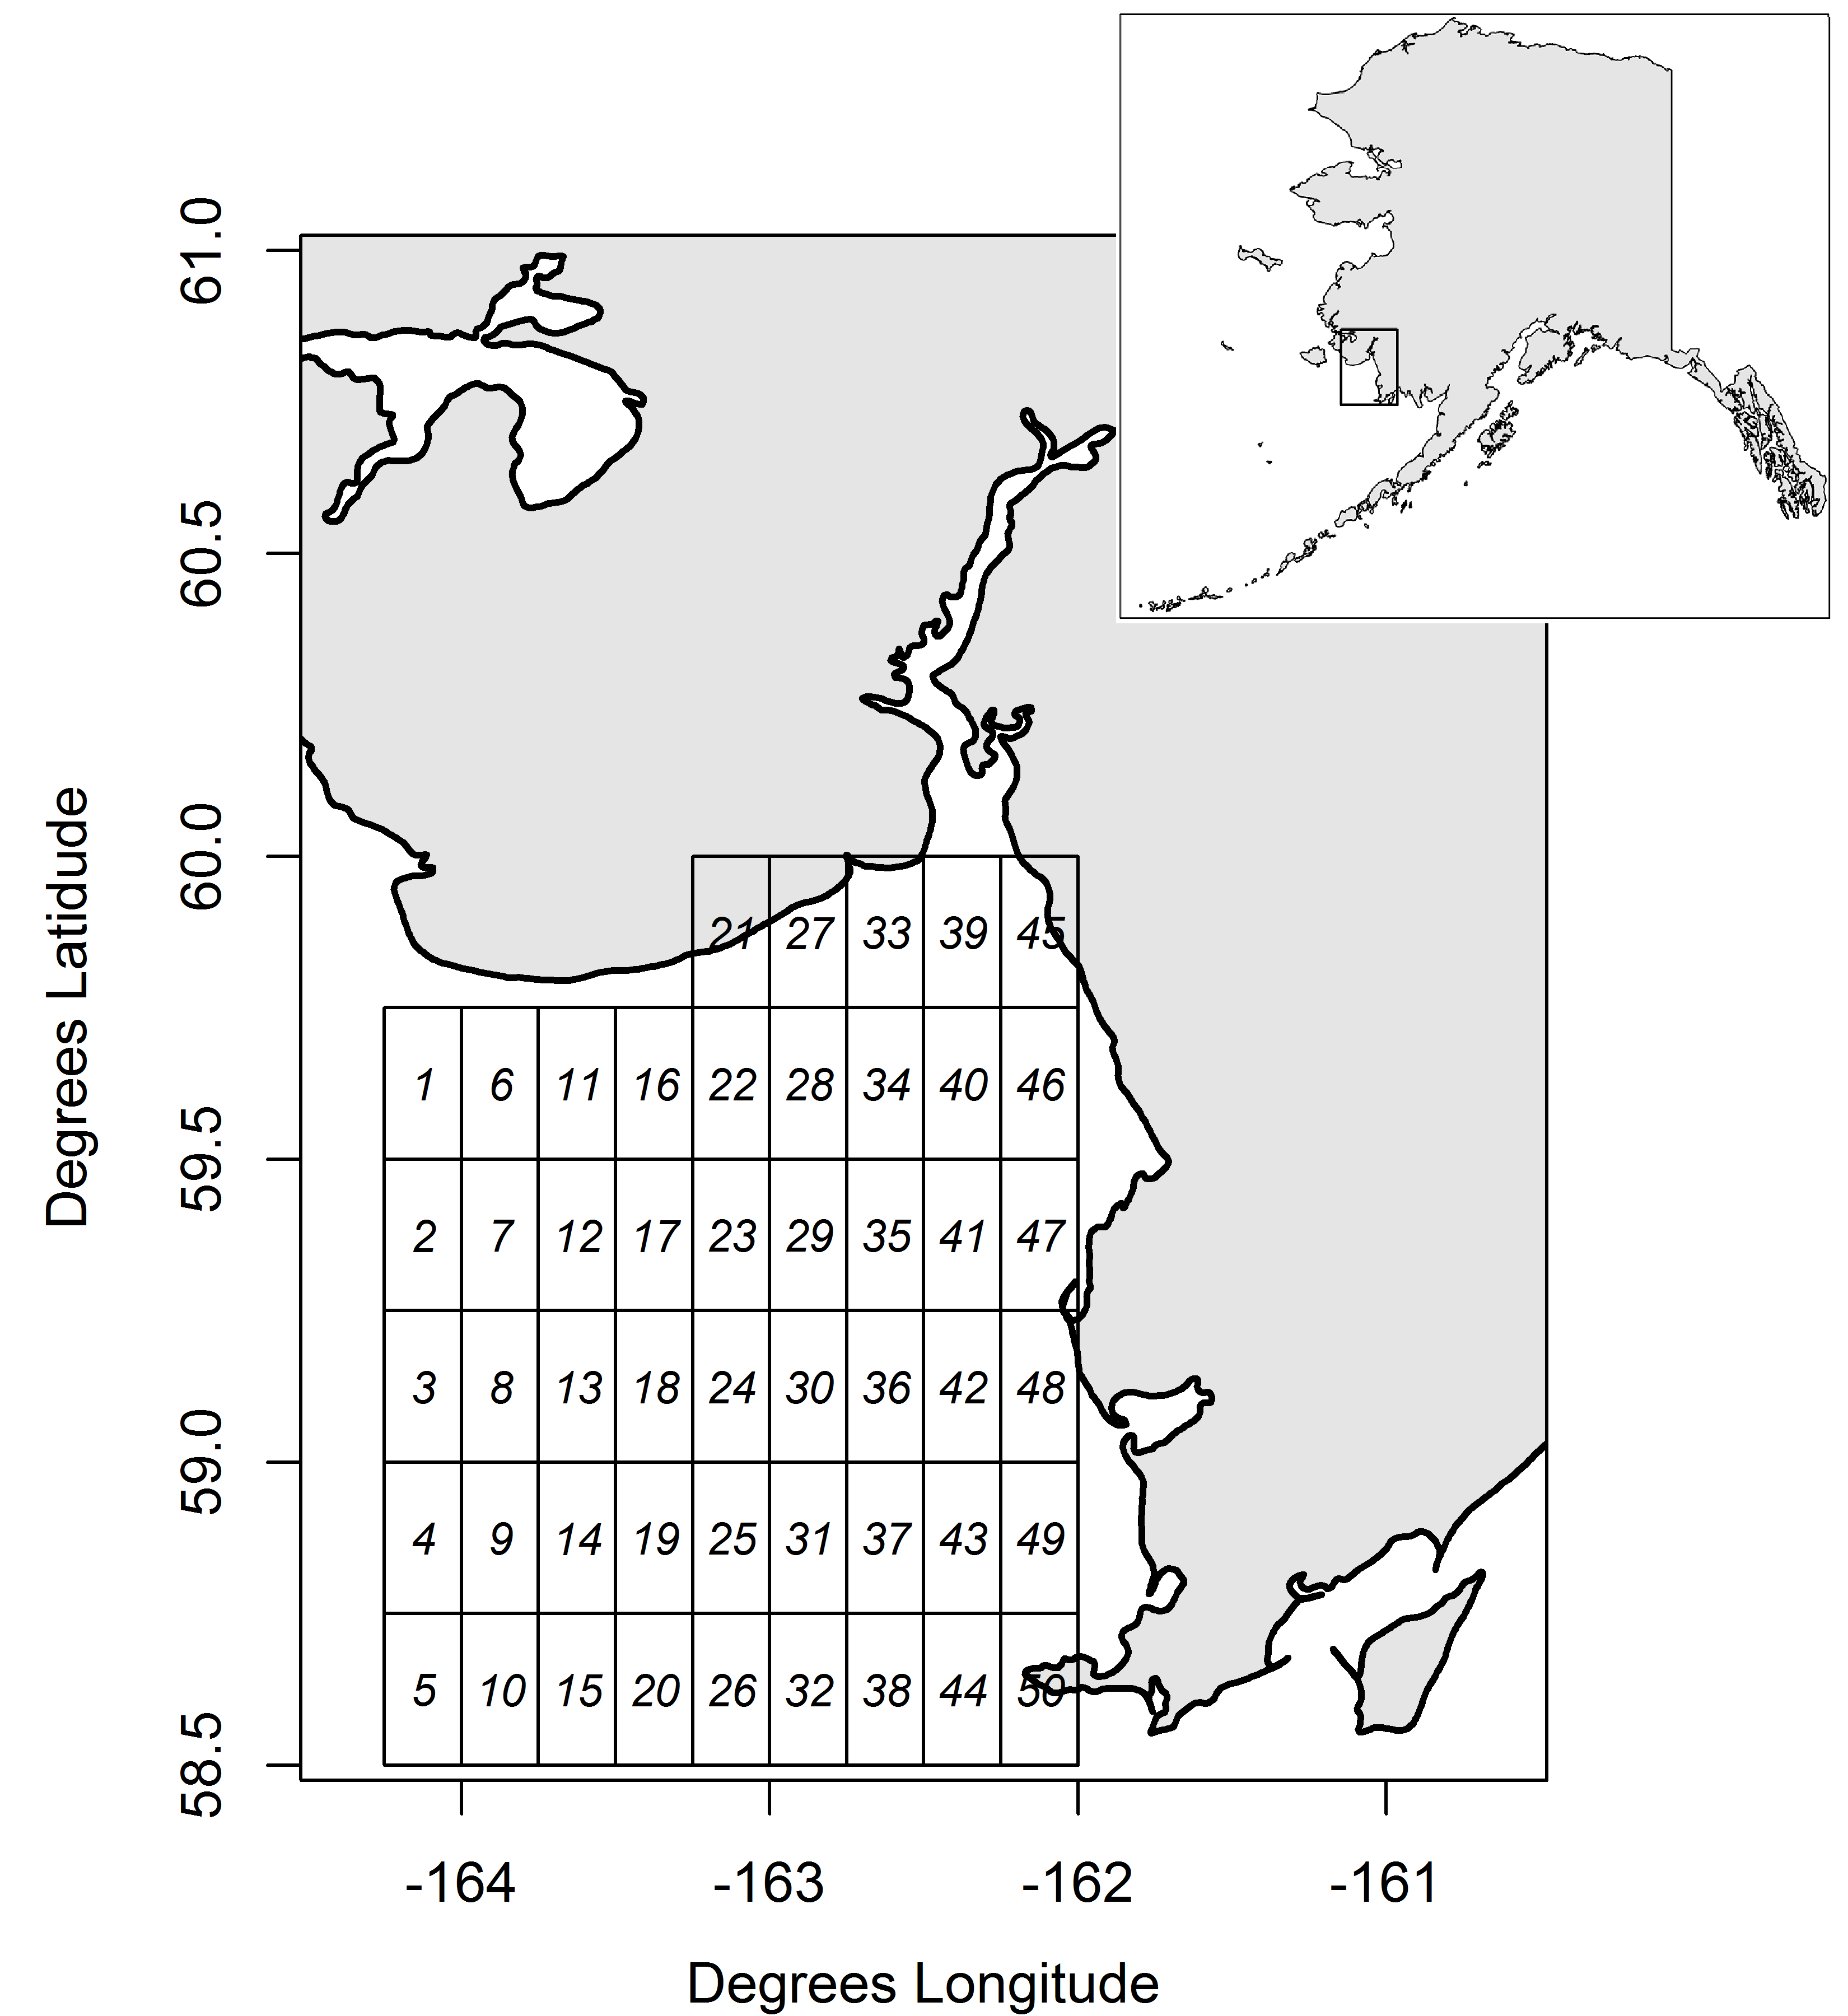
\includegraphics{img/Ch2/map.png}
  \caption{Map of Kuskokwim Bay where Chinook salmon likely stage for transition to freshwater. Shows grid cells from which daily SST values were used. Daily SIC values came from the same grid cells, though excluding grid cell 45 below due to missing values.}
  \label{fig:ch2-map}
\end{figure}

\clearpage

\hl{UPDATE THIS}

\begin{figure}
  \centering
  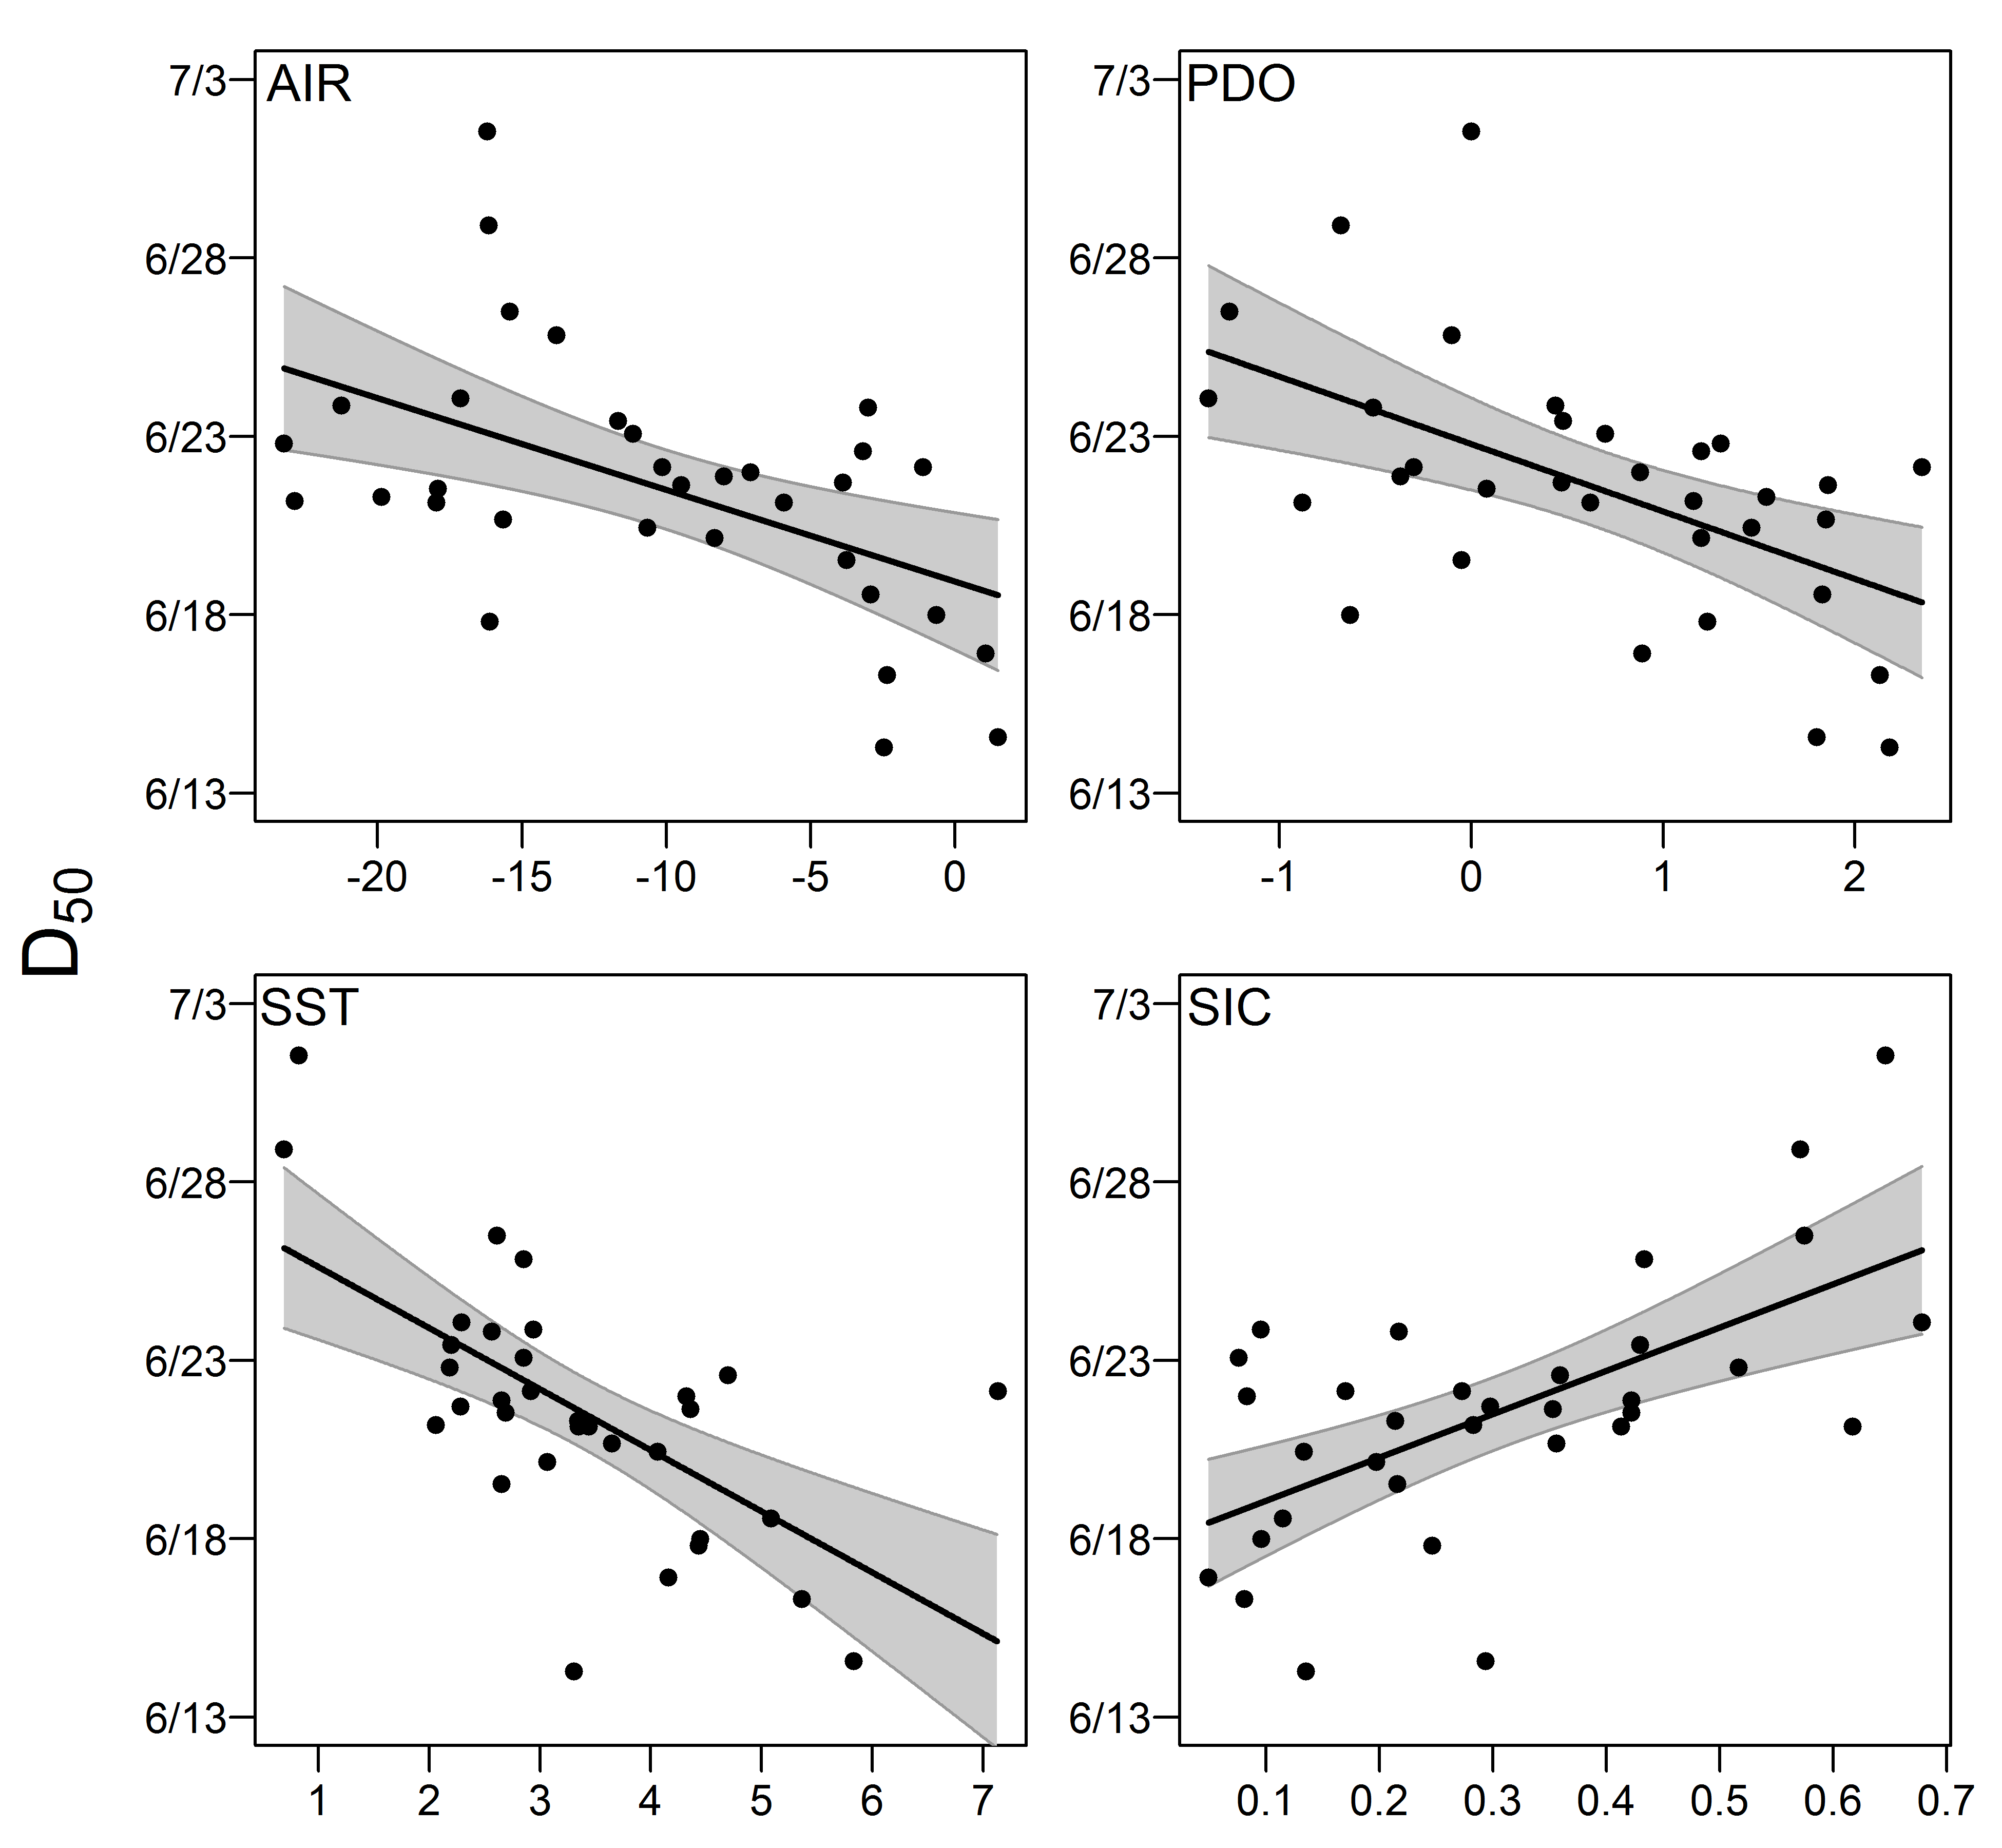
\includegraphics{img/Ch2/relationships.png}
  \caption{Relationships between the four single environmental variables and run timing $\left(D_{50}\right)$ using data from optimal climate windows when 2018 was added to the training data. For illustration purposes only, gridded variables SST and SIC were combined by weighted averaging where the weight of each grid cell was assigned the $\text{AIC}_{\text{c}}$ weight of that grid cell when grid cell-specific models were fit. Grey bands are 95$\%$ confidence intervals on the least squares line.}
  \label{fig:relationships}
\end{figure}

\clearpage

\hl{UPDATE THIS}

\begin{figure}
  \centering
  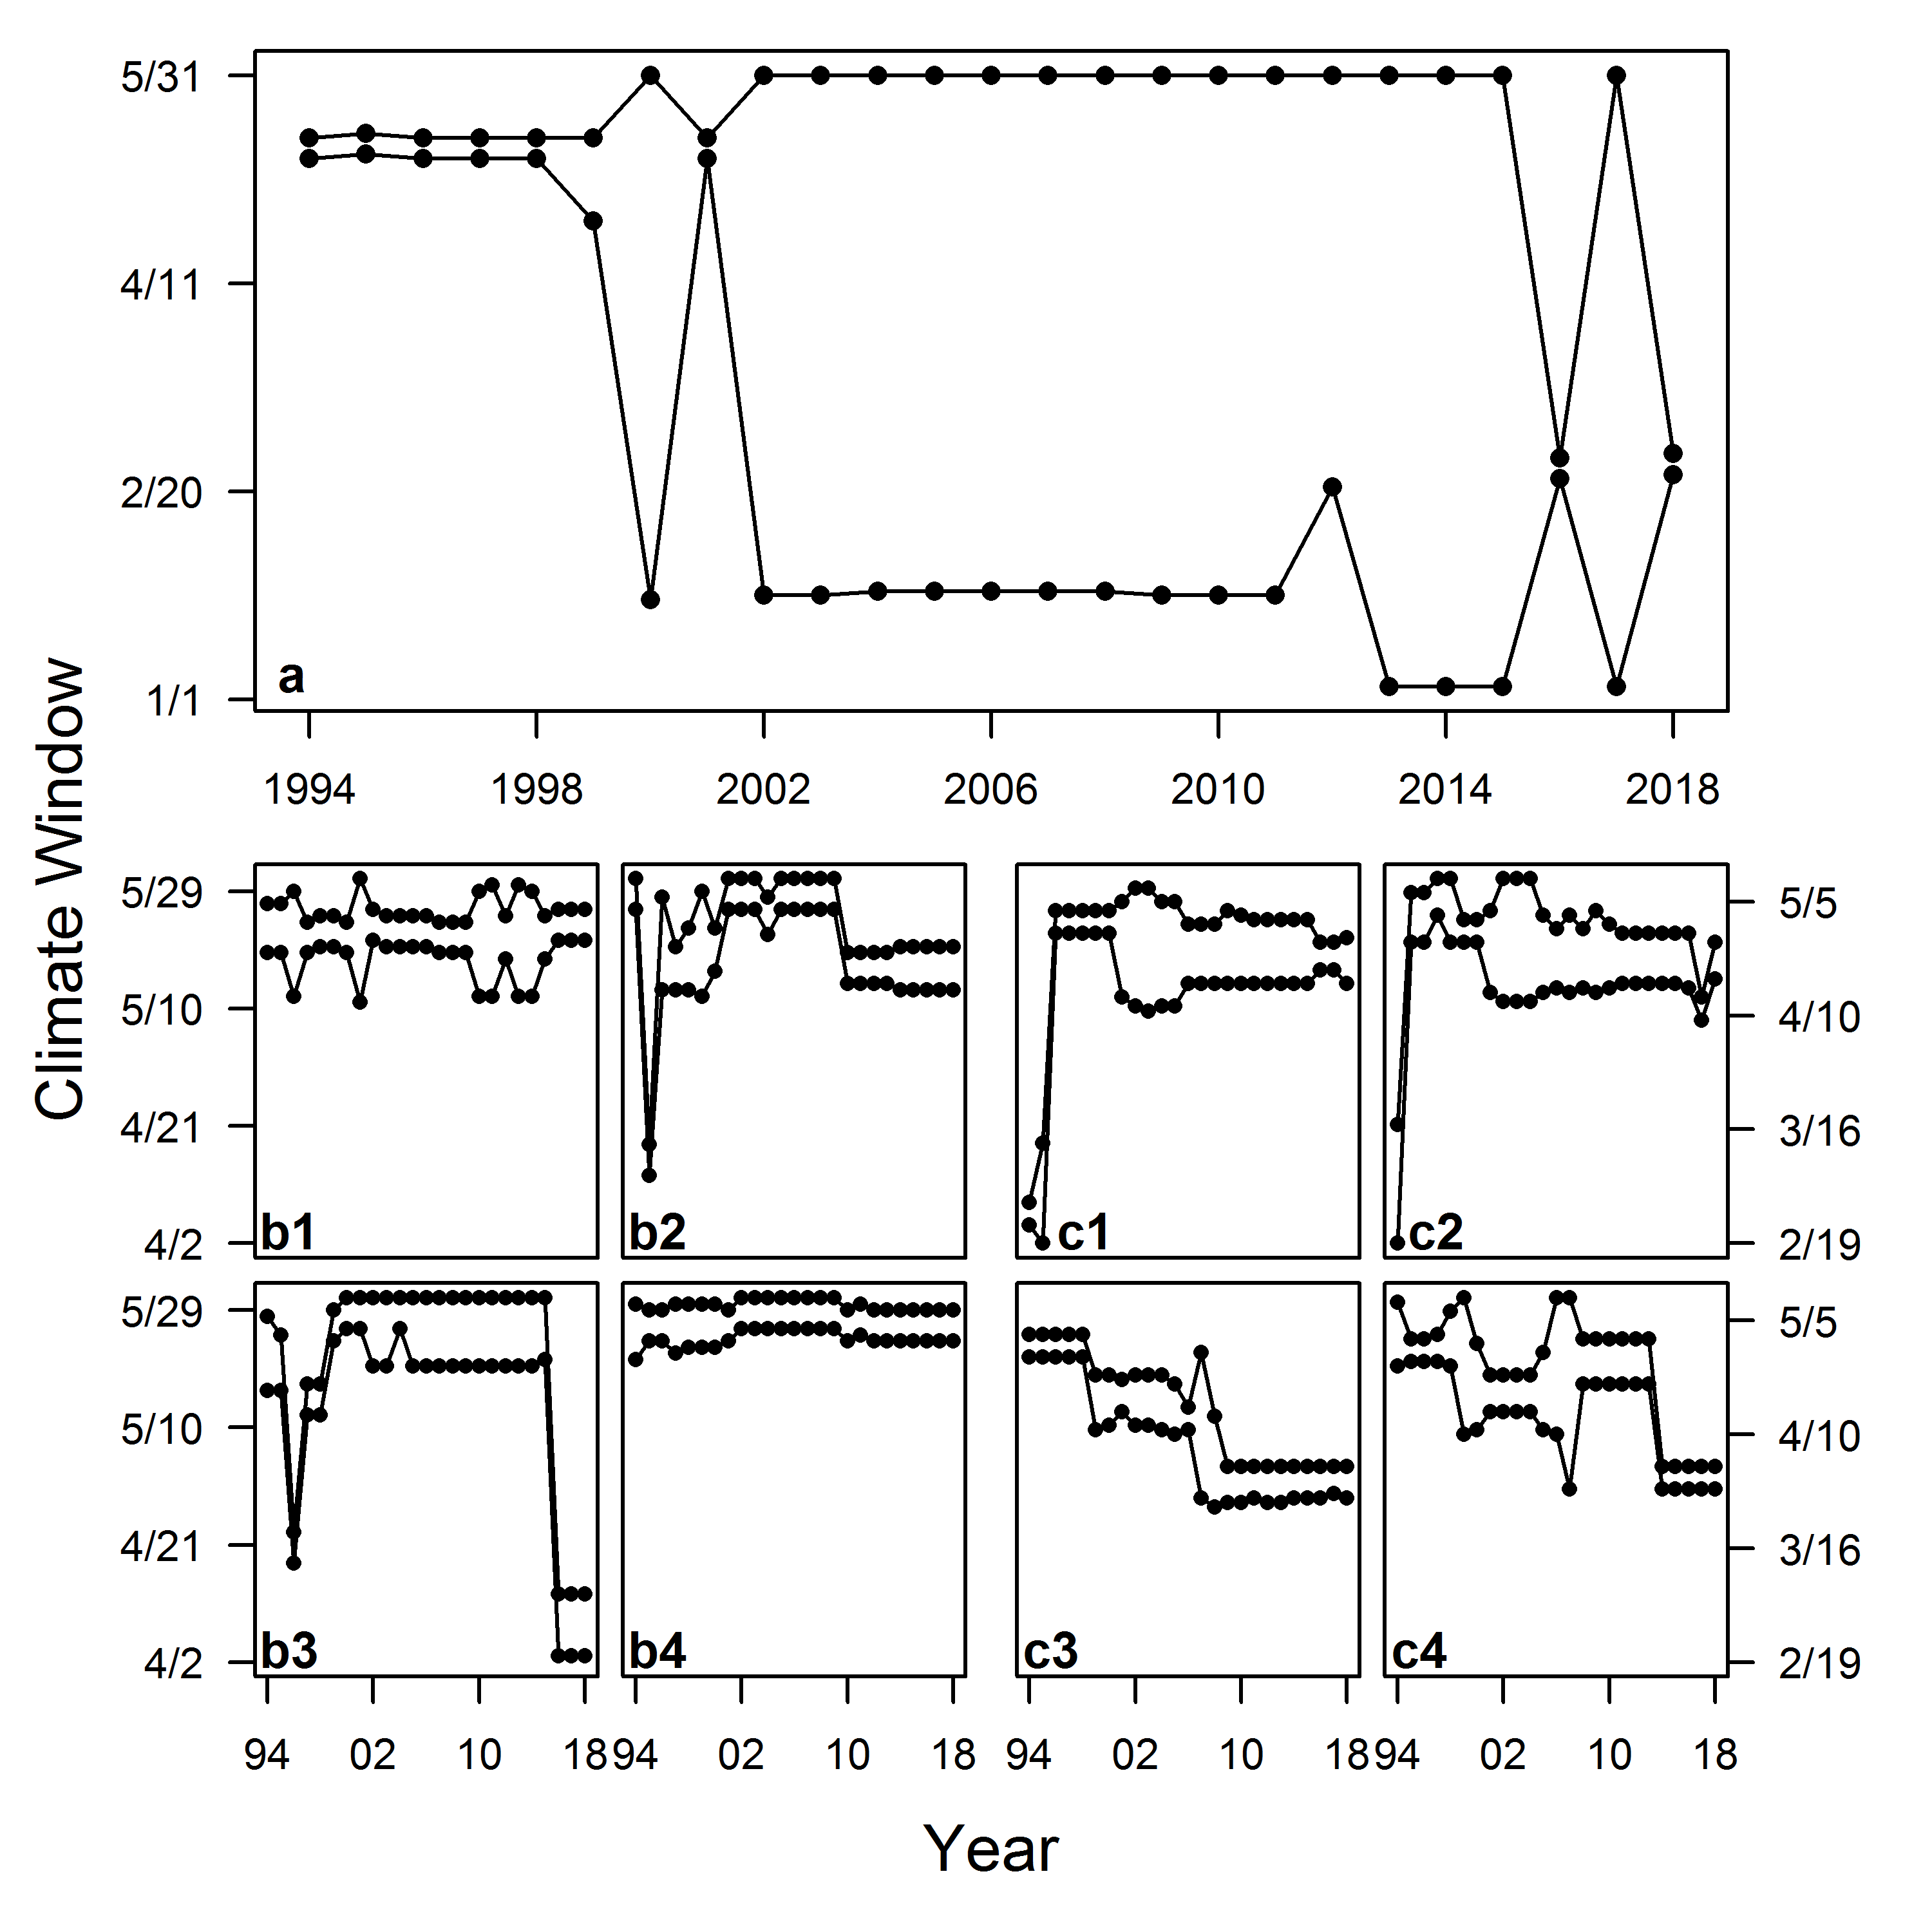
\includegraphics{img/Ch2/window-changes.png}
  \caption{Changes in selected climate windows as training data were added in the retrospective forecasting analysis. Bottom and top lines show the first and last day of the selected climate window, respectively, as more years were added. The year axis corresponds to the selected window after including environmental and run timing data from that year in the training data. E.g., the windows shown for 2017 were used to produce the forecast for 2018. Panel (a) is Bethel air temperature, panels b1-b4 are SST windows for four sample grid cells and panels c1-c4 are SIC windows for the same four sample grid cells. Sample grid cells from Figure \ref{fig:ch2-map} shown for SST and SIC are as follows: grid cell 8 (b1, c1), grid cell 44 (b2, c2), grid cell 12 (b3, c3), and grid cell 48 (b4, c4). Selected windows for PDO are not shown because the single month of May was selected in all years.}
  \label{fig:window-changes}
\end{figure}

\clearpage

\hl{UPDATE THIS}

\begin{figure}
  \centering
  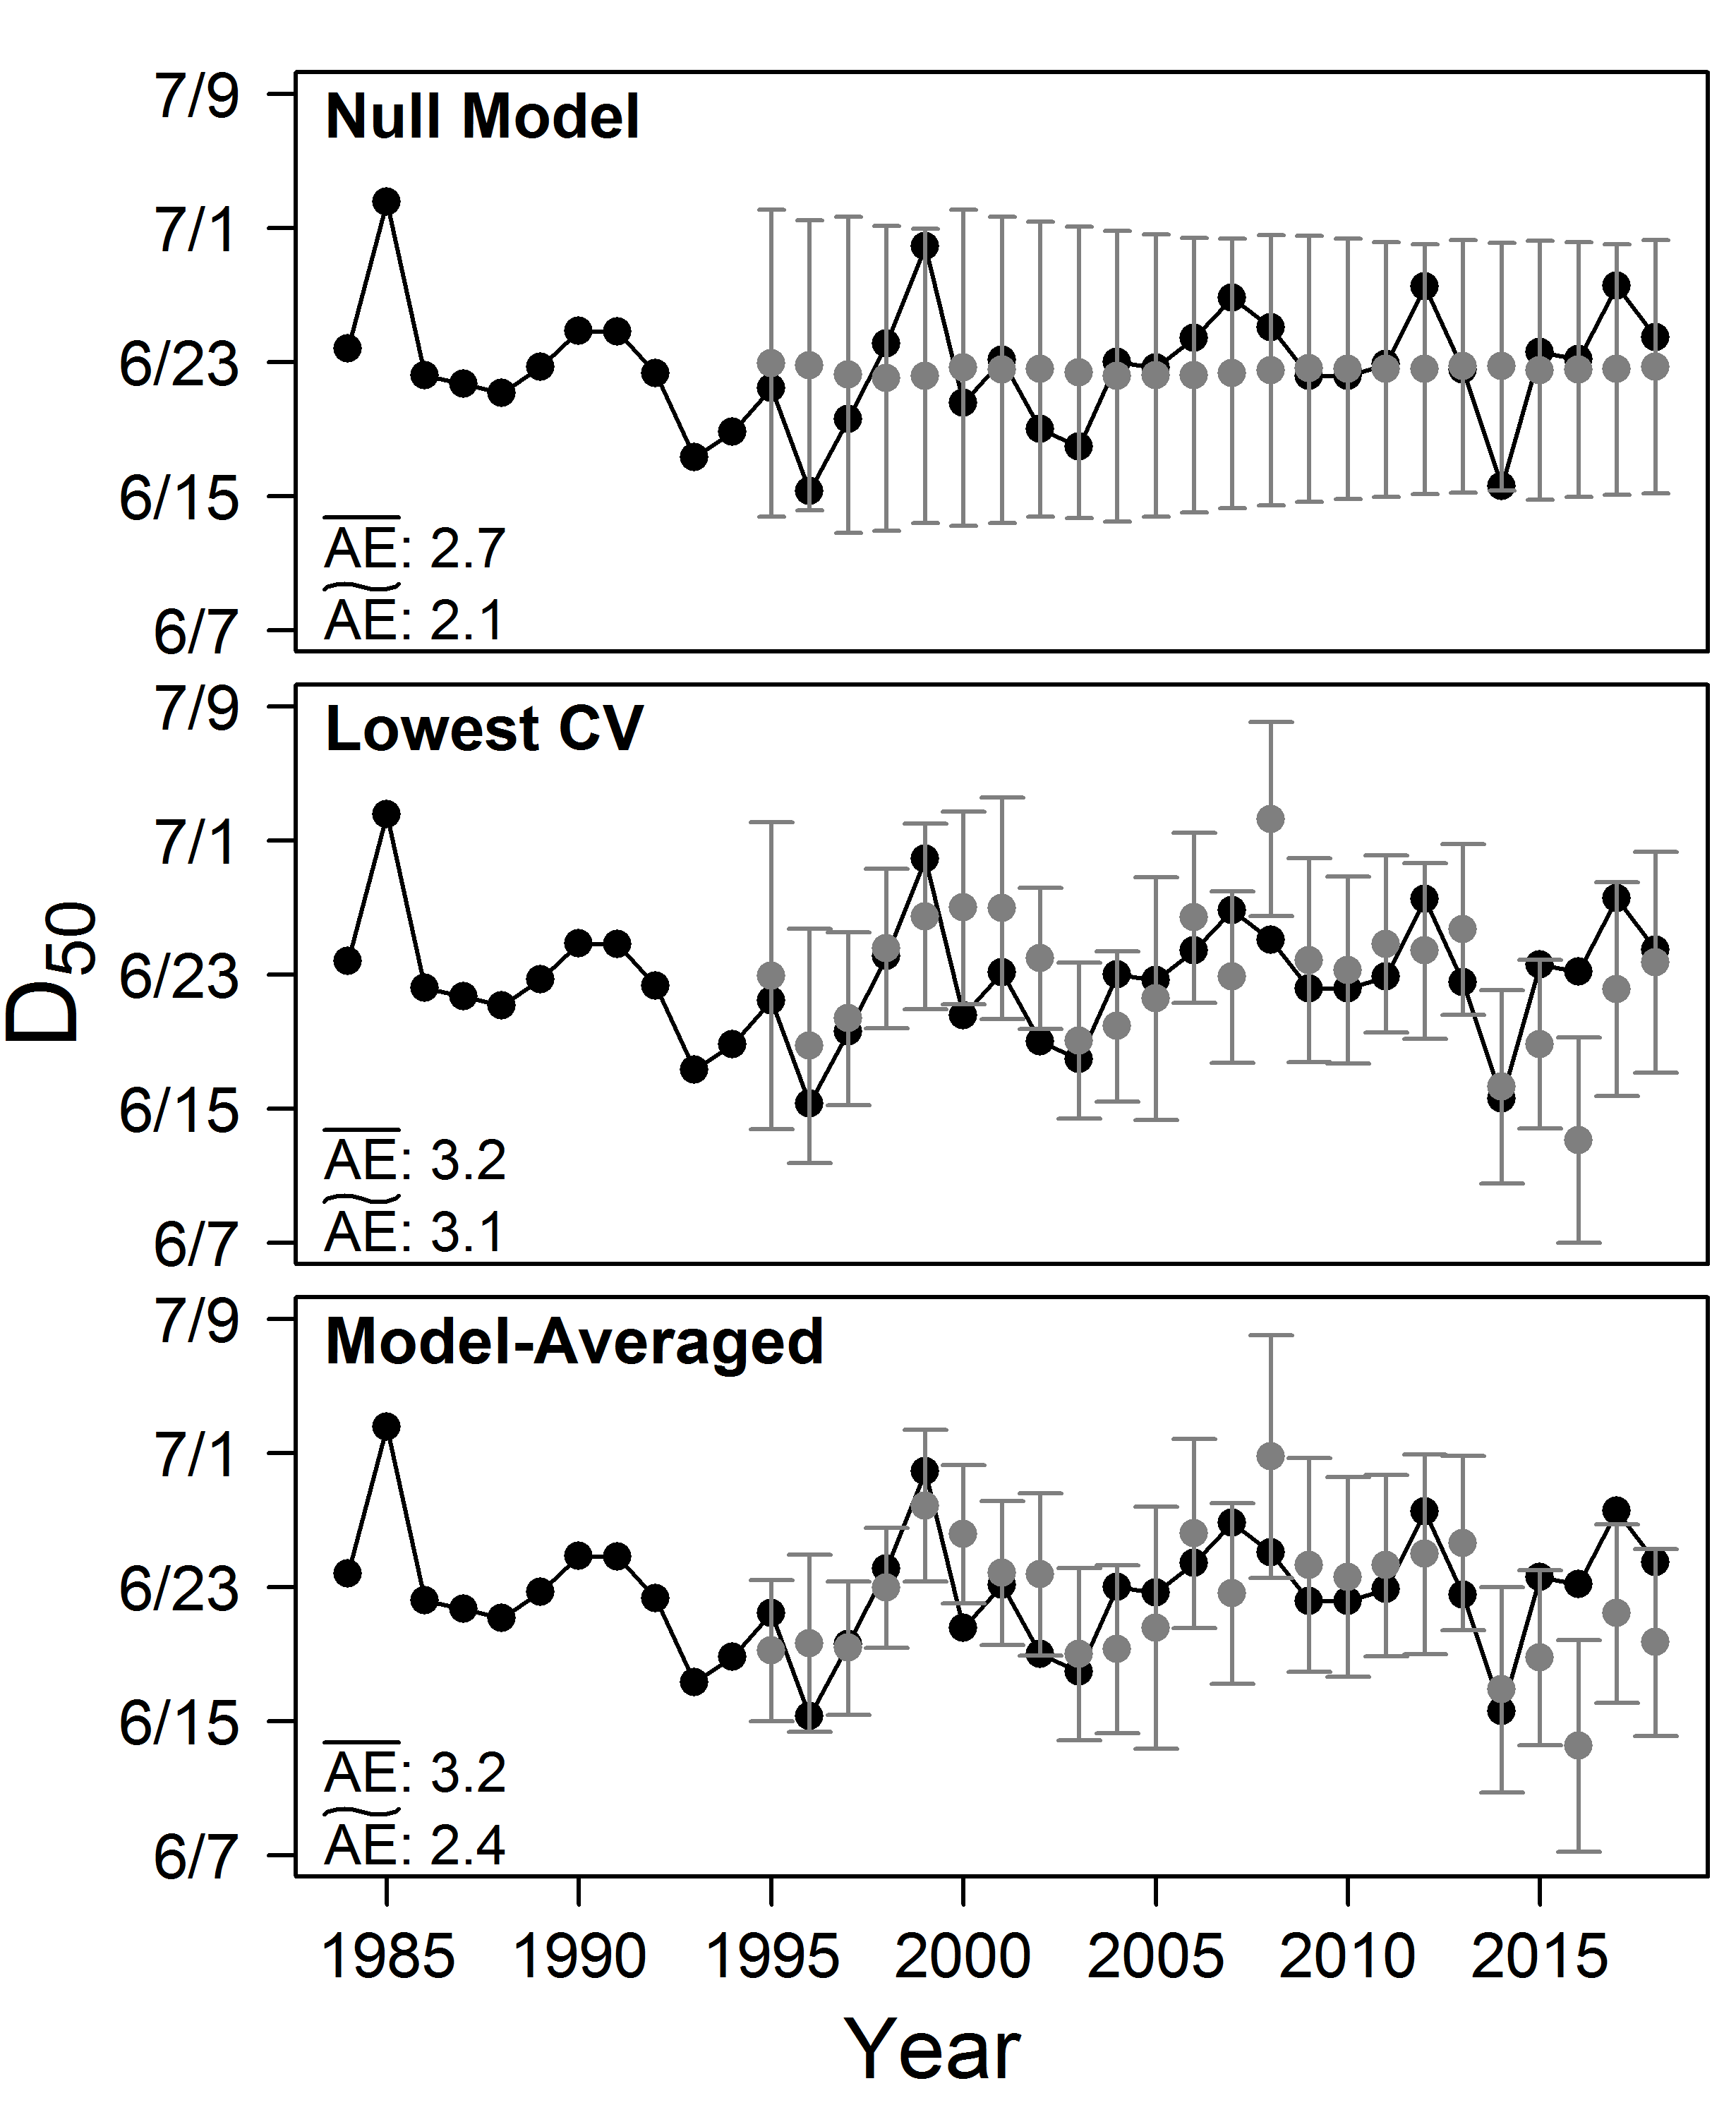
\includegraphics{img/Ch2/forecasts.png}
  \caption{Produced forecasts under the three approaches. Black points/lines are the time series of $D_{50}$ detected by the BTF. Grey points are out-of-sample forecasts with 95$\%$ prediction intervals shown as error bars. $\overline{\text{AE}}$ and $\widetilde{\text{AE}}$ are the mean and median absolute forecast errors from 1995 to 2018, respectively.}
  \label{fig:forecasts}
\end{figure}

\clearpage

\hl{UPDATE THIS}

\begin{figure}
  \centering
  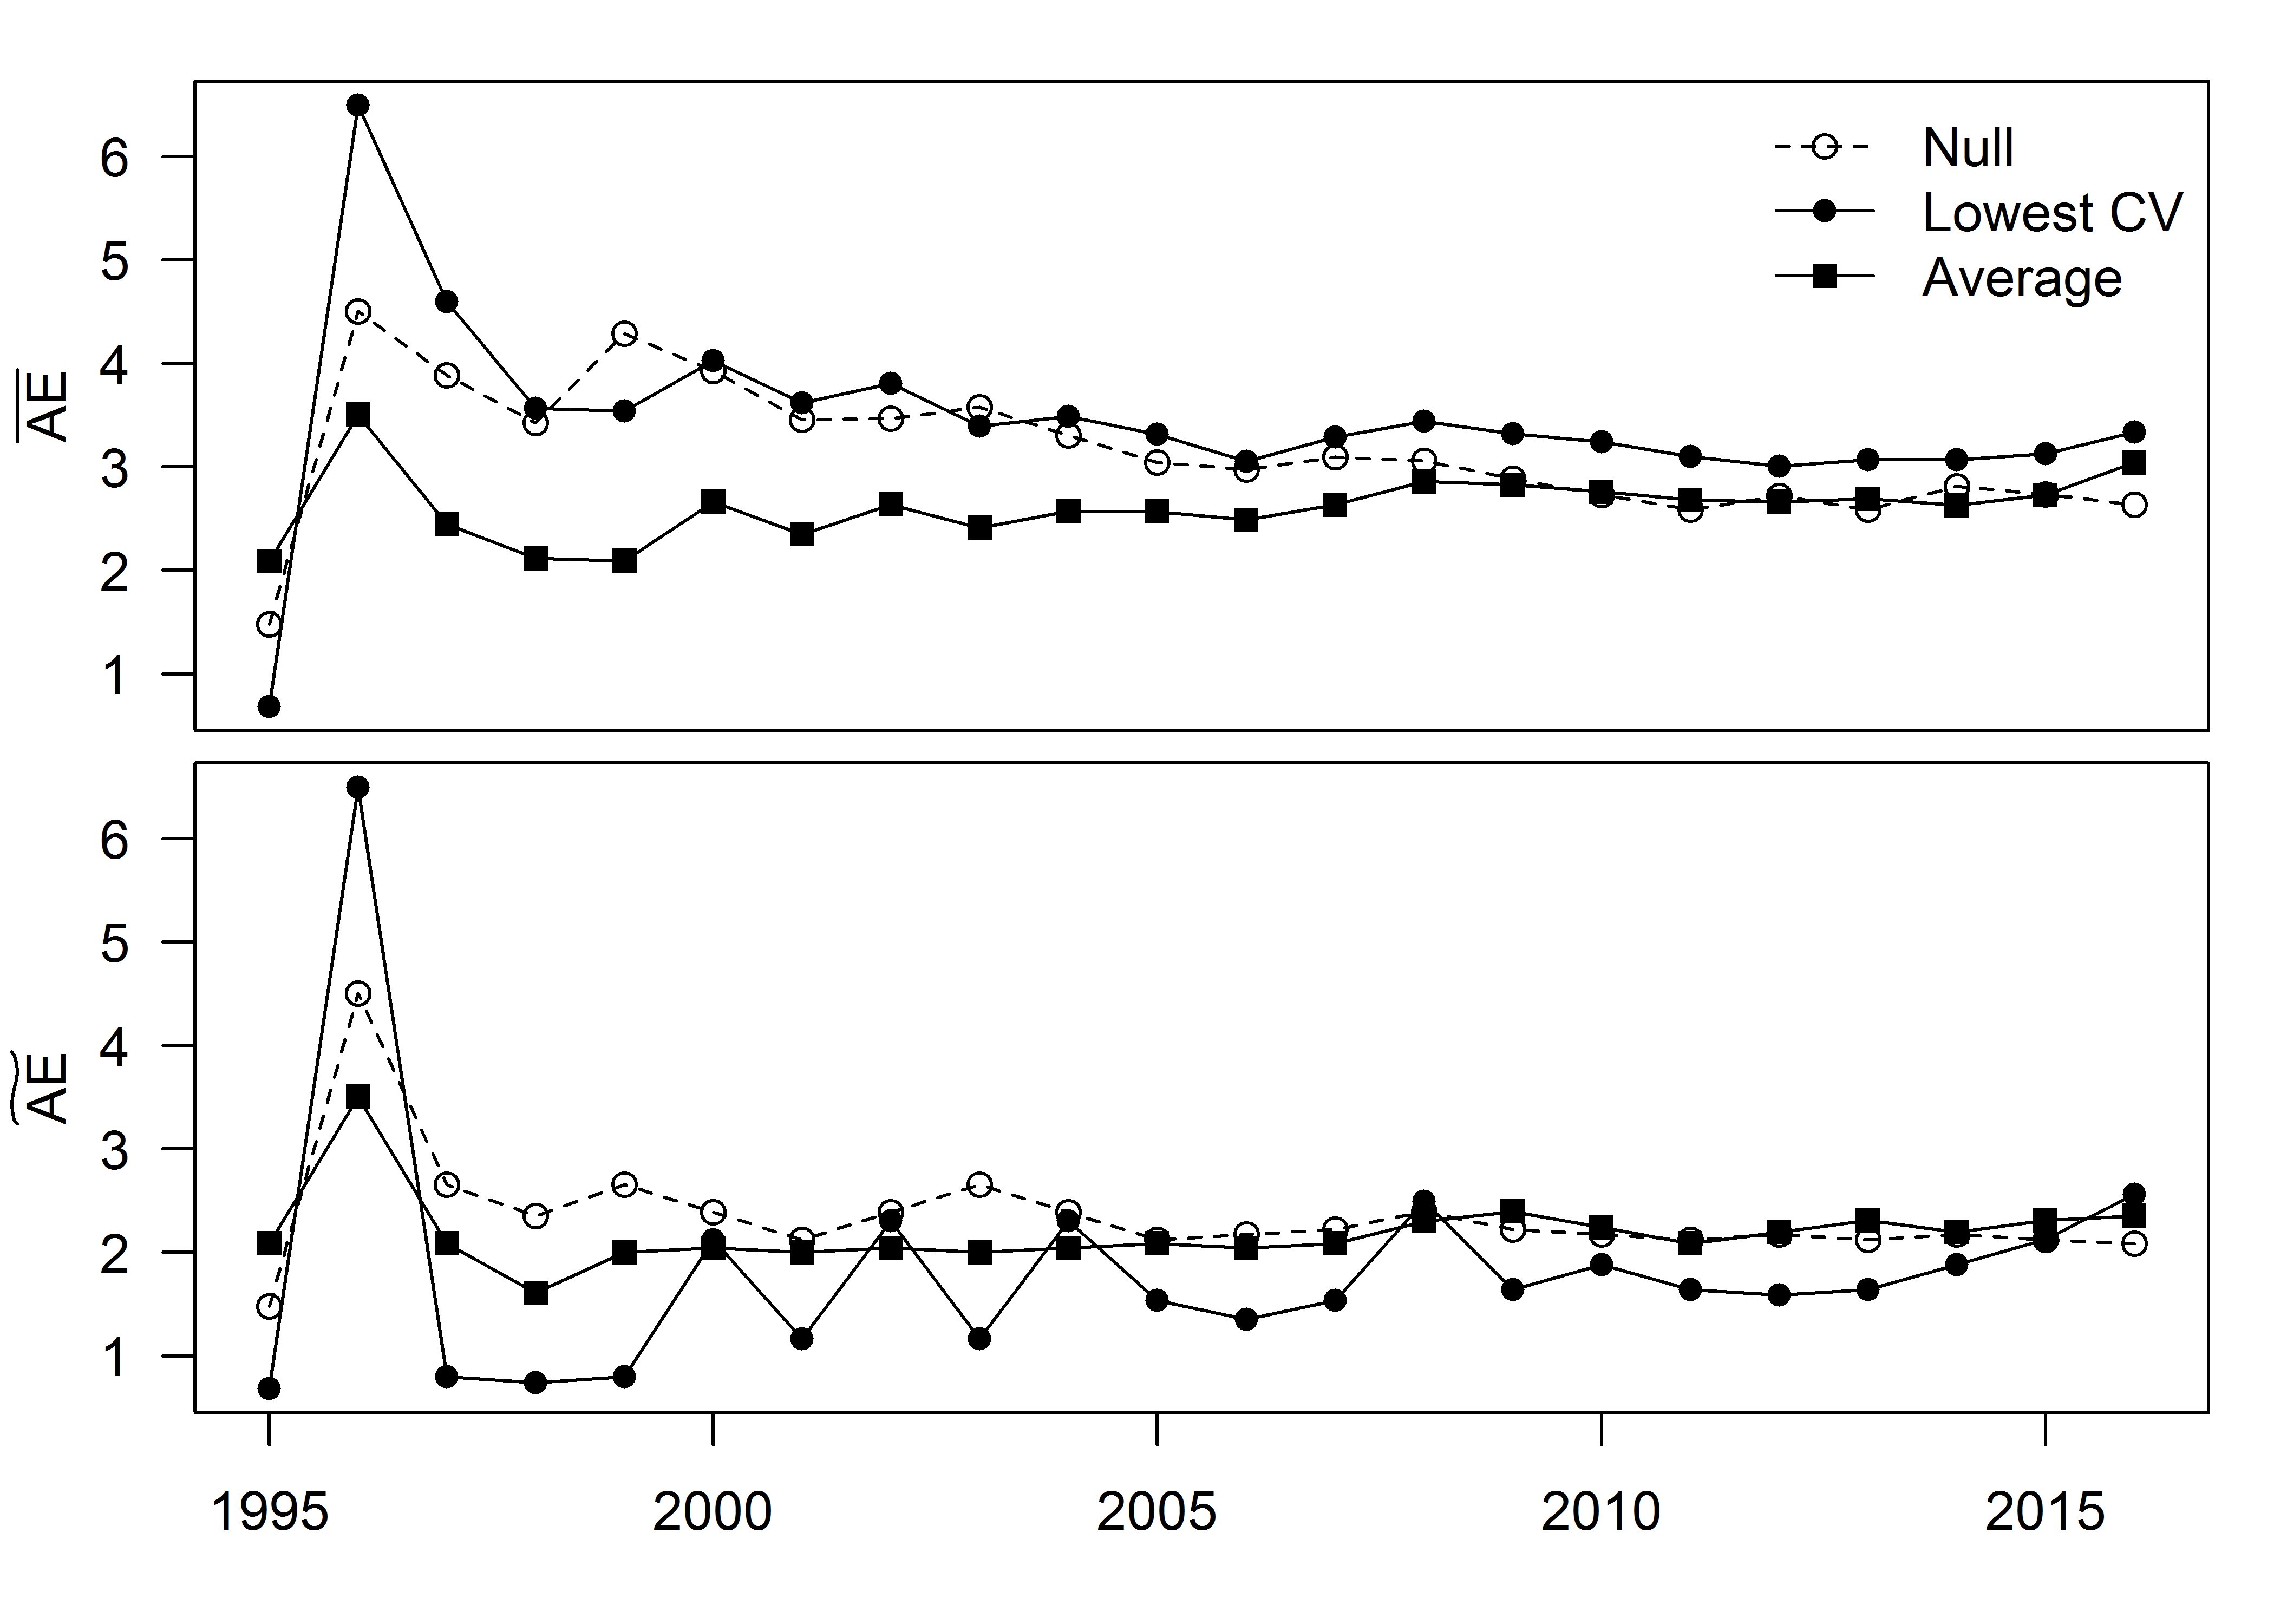
\includegraphics{img/Ch2/ae-changes.png}
  \caption{Evolution of $\overline{\text{AE}}$ (mean) and  $\overline{\text{AE}}$ (median) absolute forecast error under the three investigated forecasting approaches. Each point is the average of absolute errors of all years before and including the corresponding year on the x-axis, starting in 1995.}
  \label{fig:ae-changes}
\end{figure}

\clearpage

\hl{UPDATE THIS}

\begin{figure}
  \centering
  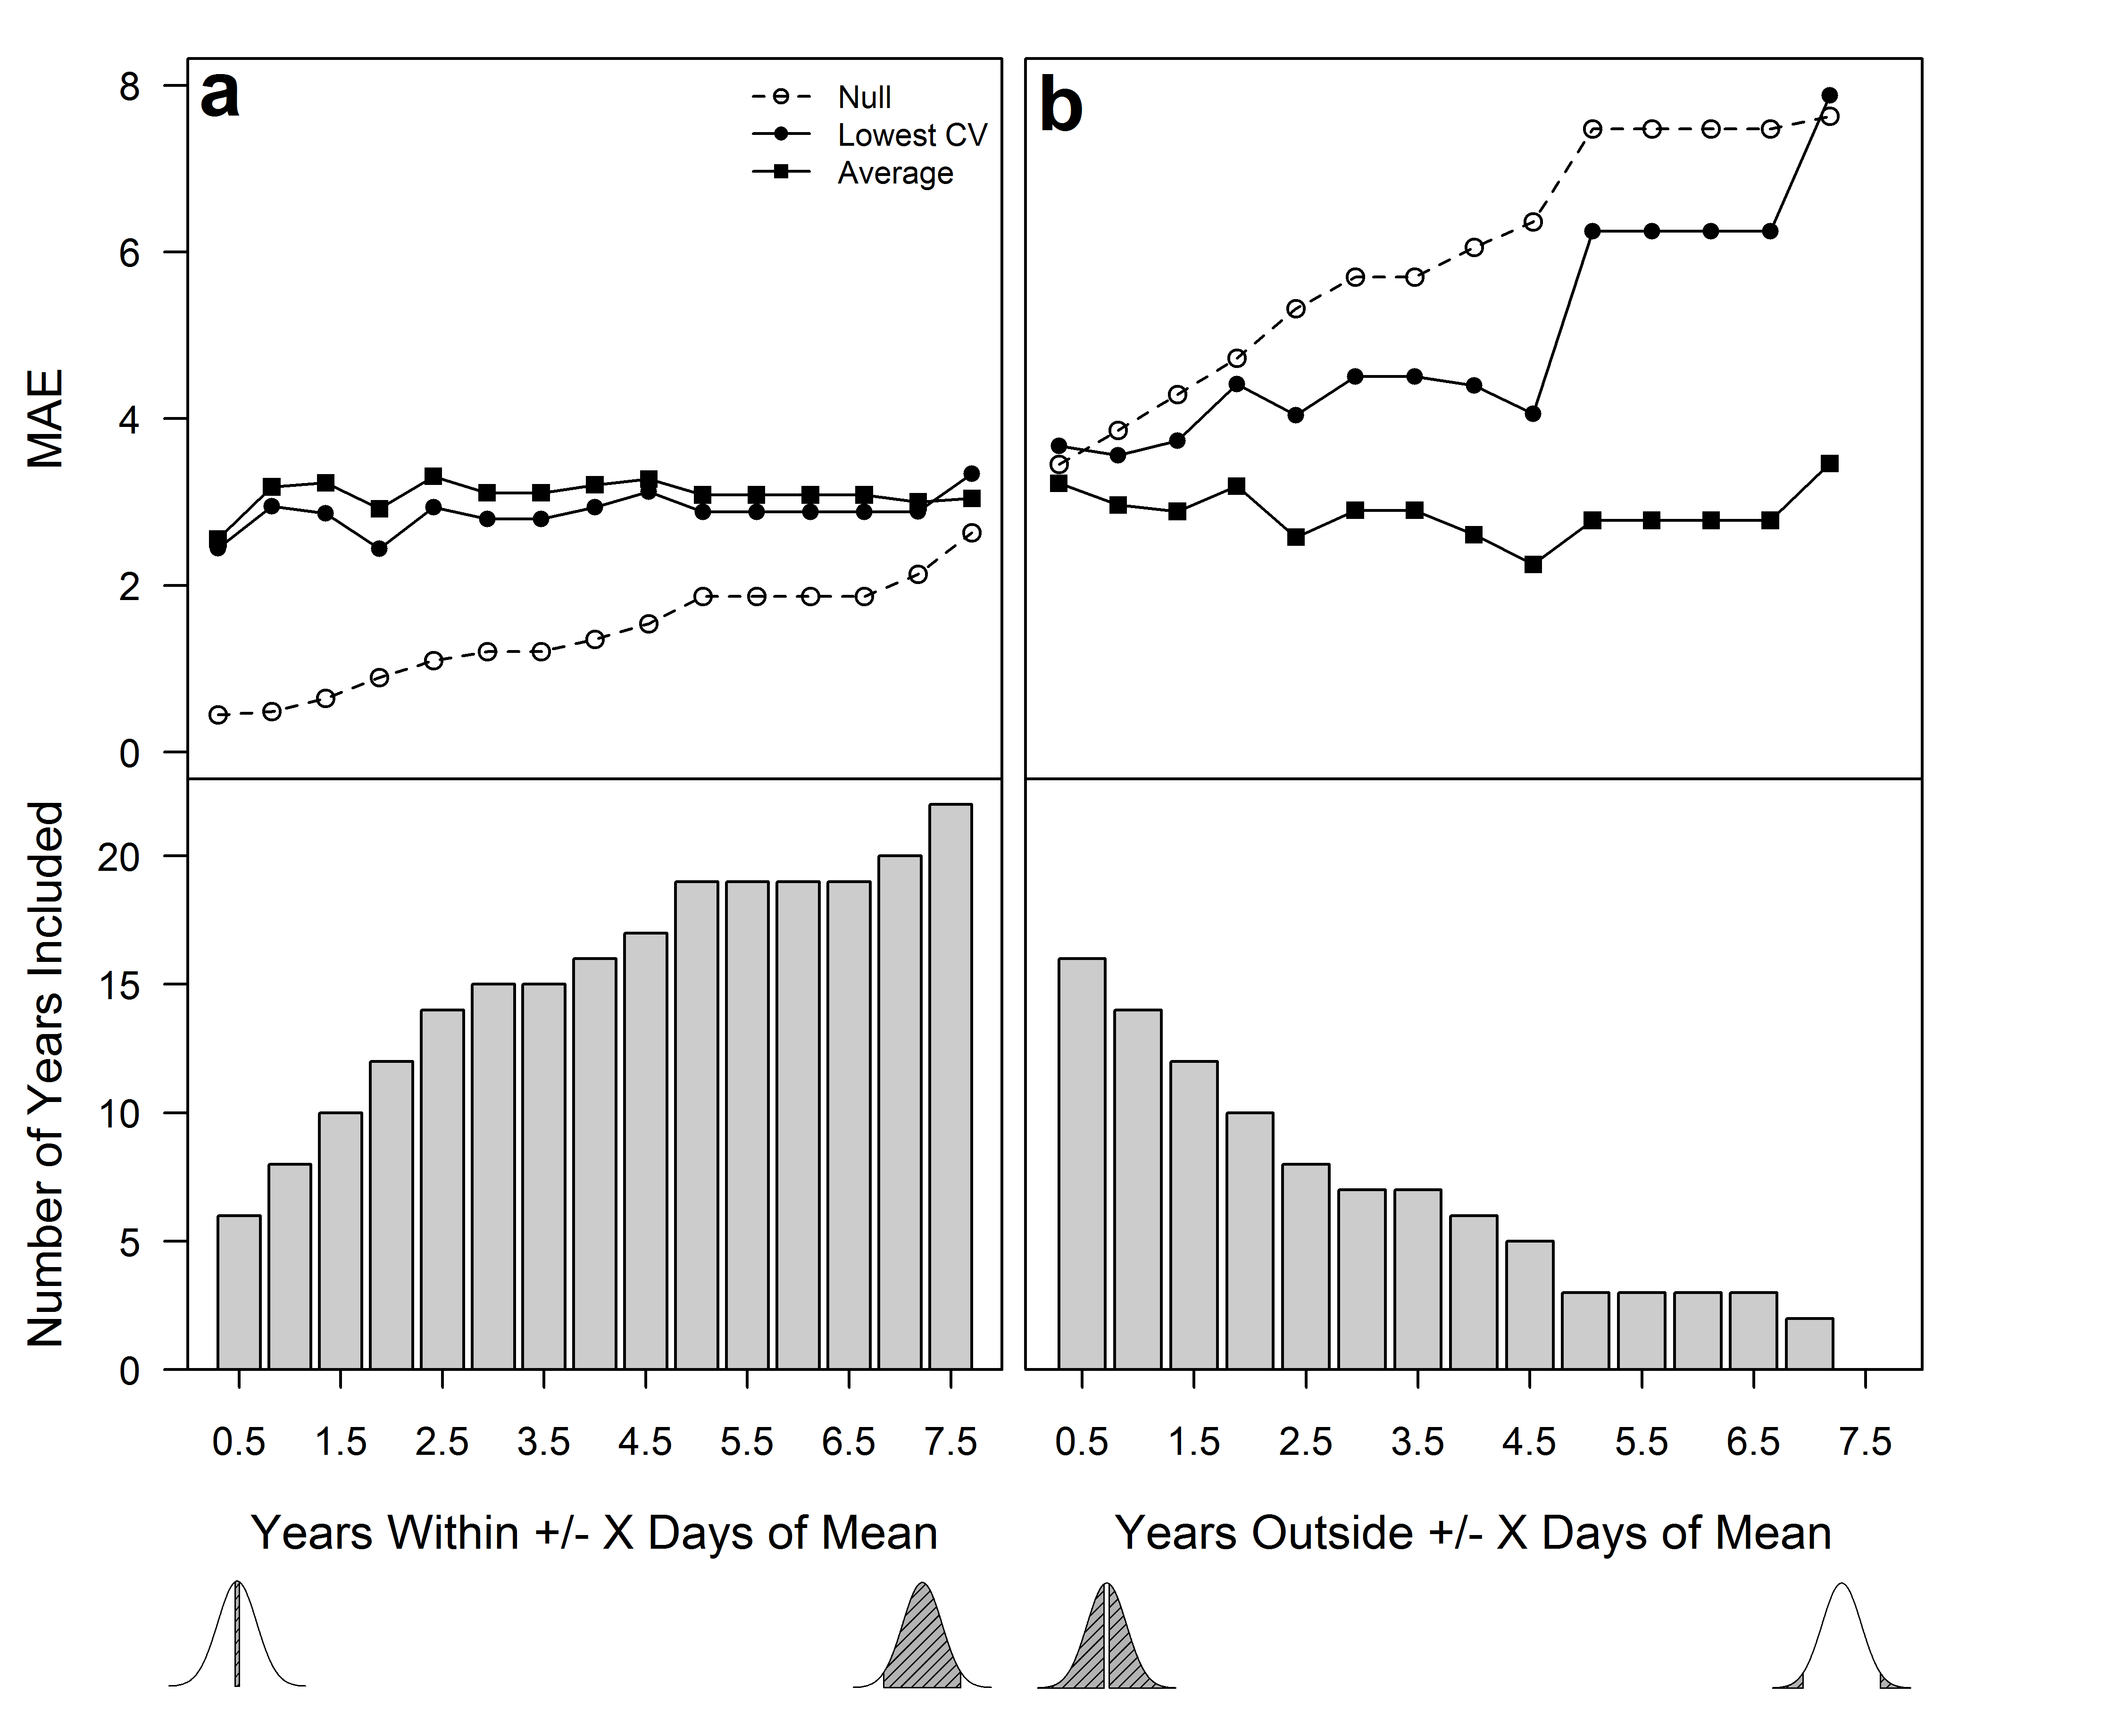
\includegraphics{img/Ch2/mae-subsets.png}
  \caption{$\overline{\text{AE}}$ under three forecast approaches calculated by either (a) including years with a $D_{50}$ value within $\pm x$  days of the all-year average or (b) including years with a $D_{50}$ value outside $\pm x$ days of average, where $x$ is the number of days indicated on the $x$-axis. Bottom panels show the number of observed years in which the appropriate $\pm x$ days criterion was met. Shaded regions in the hypothetical distributions show the types of $D_{50}$ values that were included in the calculation of $\overline{\text{AE}}$. One point that may enrich inference from this figure (and is shown in the shaded normal distributions) is that panel (a) becomes more inclusive from left to right by adding years that are more dissimilar to the average in the calculation of $\overline{\text{AE}}$ whereas panel (b) becomes more exclusive from left to right by removing years that are similar to the average.}
  \label{fig:mae-subsets}
\end{figure}

\clearpage

\hl{UPDATE THIS}

\begin{figure}
  \centering
  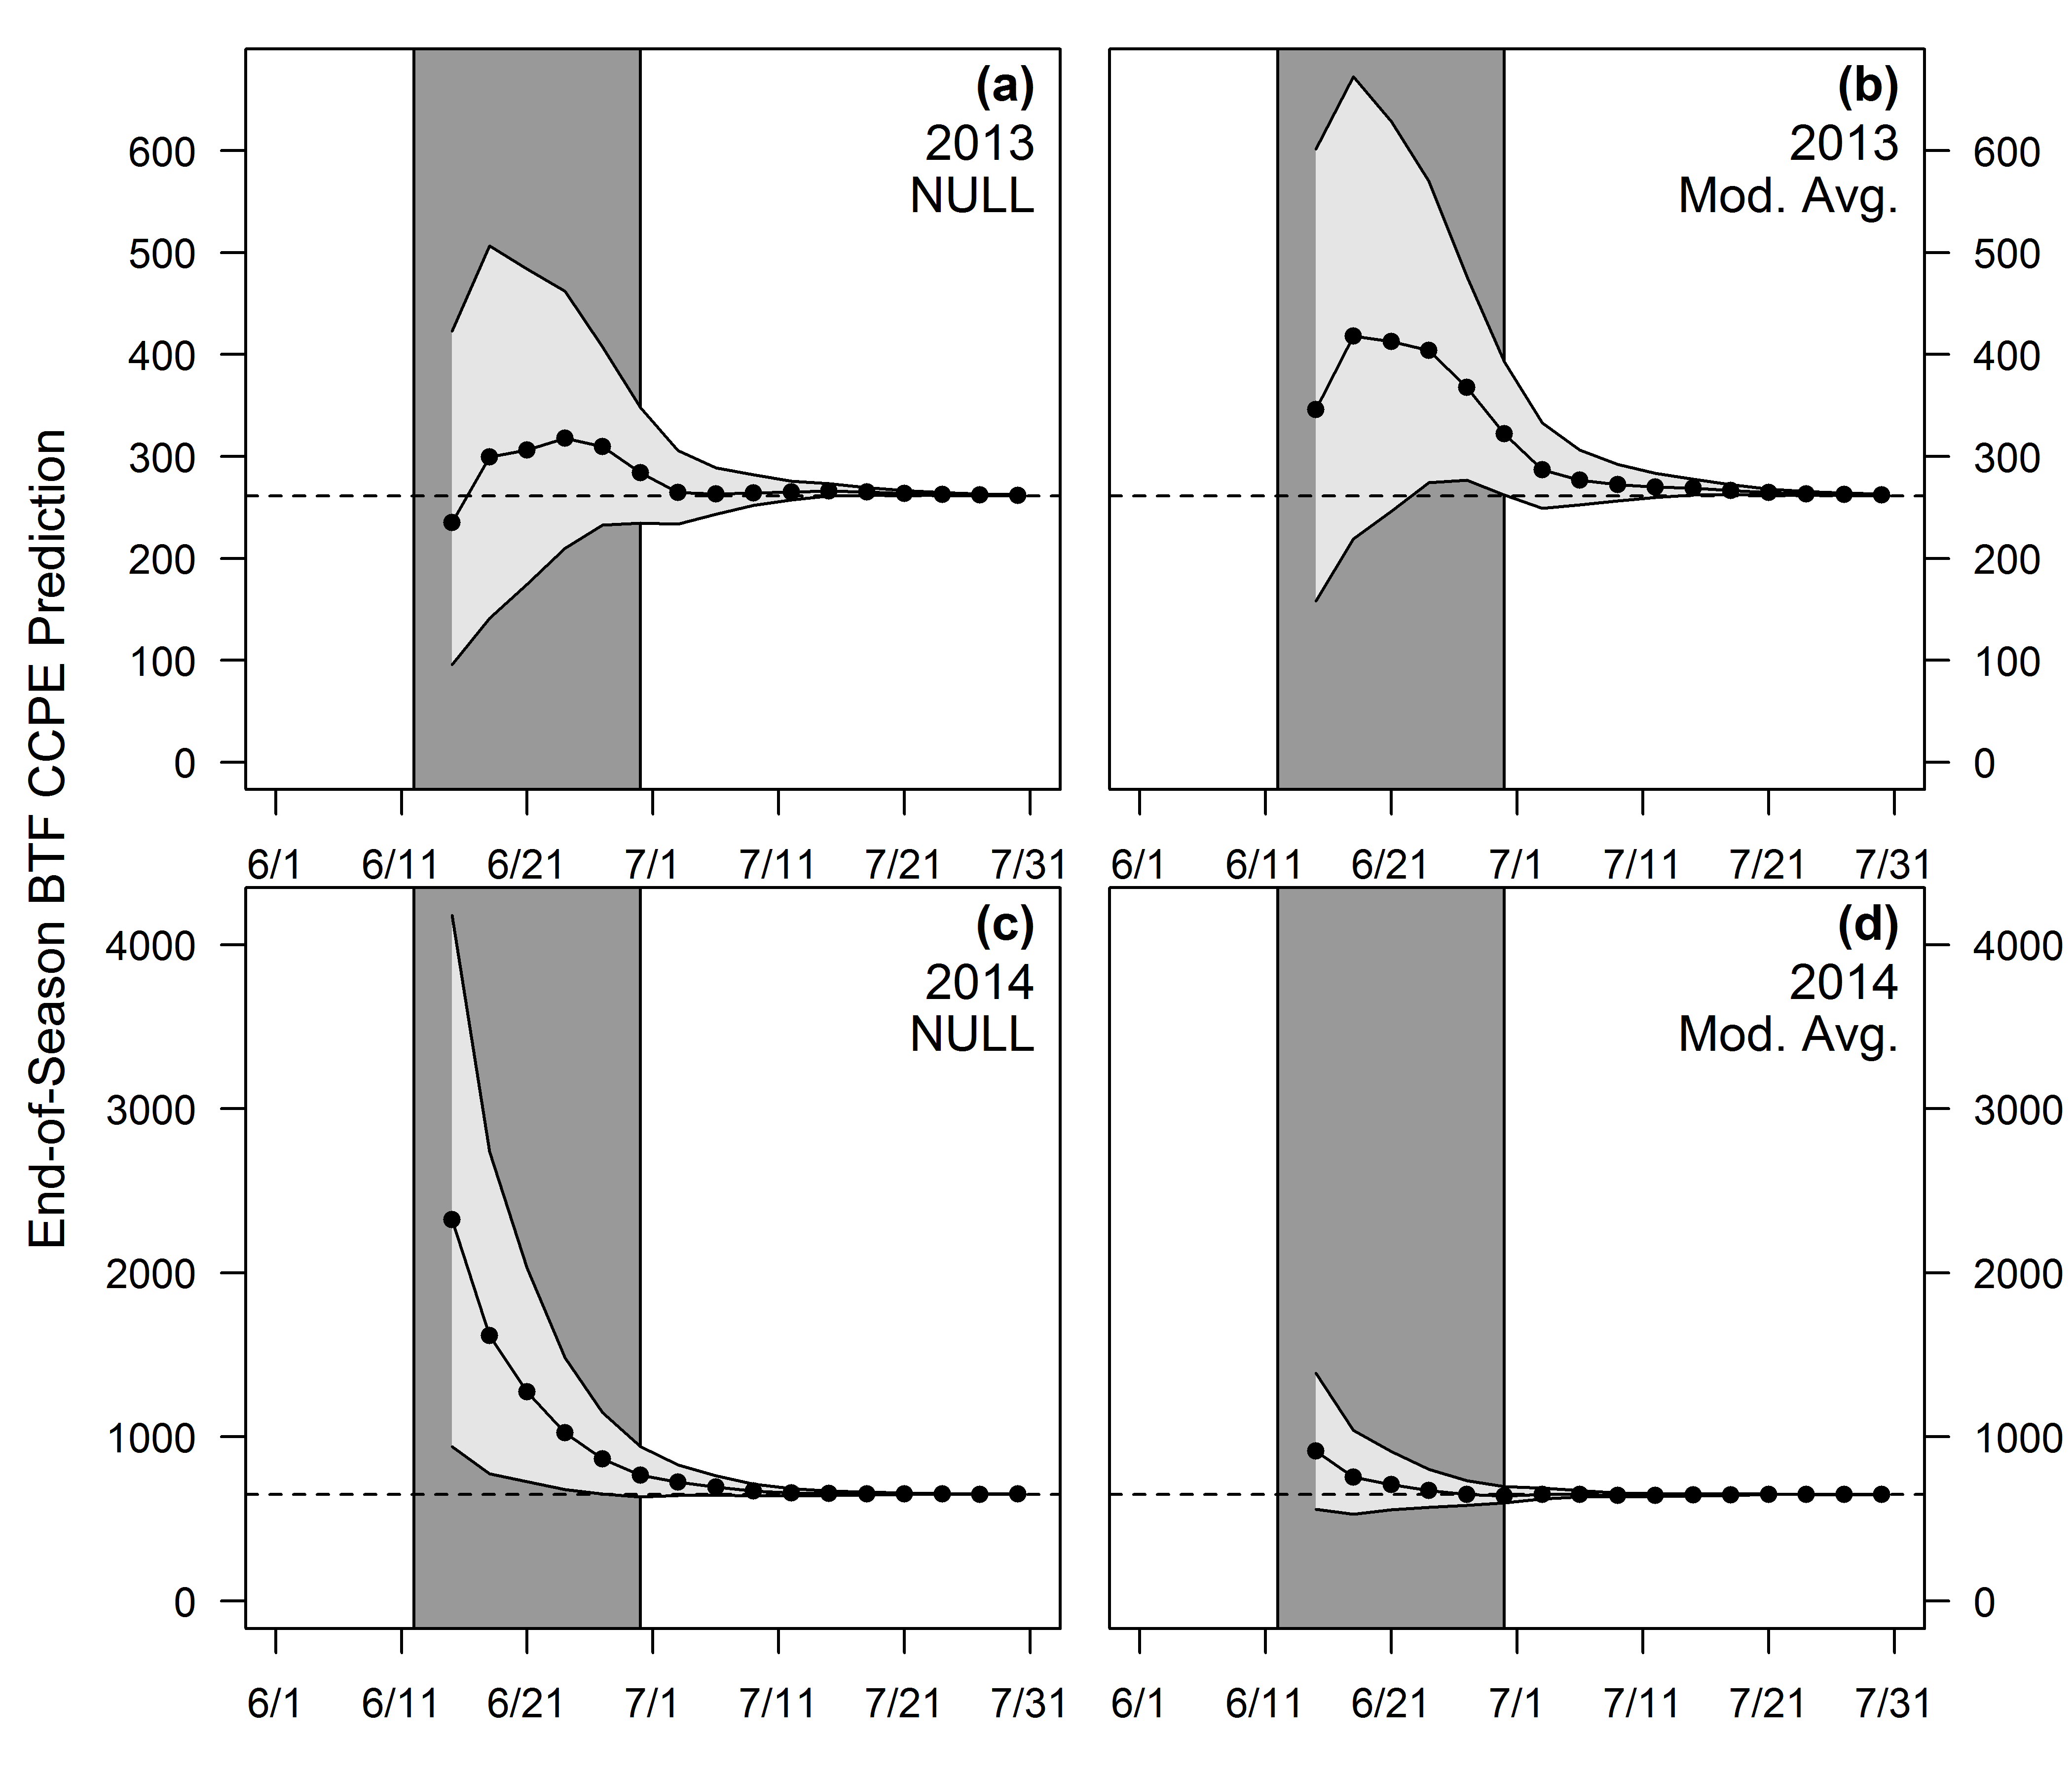
\includegraphics{img/Ch2/eos-preds.png}
  \caption{In-season predictions of end of season cumulative BTF CPUE under the model-averaged forecast using environmental variables and the forecast under the null model in 2013 and 2014. Intended to illustrate cases in which a manager would benefit from having access to the model-averaged run timing forecast model using environmental variables (2014) and when the null model would have performed better (2013). Horizontal lines are the true end of season cumulative BTF CPUE, dark grey regions are 50$\%$ confidence intervals, and light grey regions are 95$\%$ confidence intervals. Grey vertical lines indicate the period when key harvest decisions are made.}
  \label{fig:eos-preds}
\end{figure}

\chapter{Evaluation of Intra-Annual Harvest Control Rules via
Closed-Loop Simulation}\label{ch3}

\section{Introduction}\label{introduction-1}

Here's chapter 3. It's about in-season simulation models for management
strategy evaluations.

\section{Methods}\label{methods-1}

I did some stuff.

\section{Results}\label{results-1}

I found some stuff.

\section{Discussion}\label{discussion-1}

Here's what it means.

\begin{singlespace}

\begin{table}[H]
\centering\rowcolors{2}{gray!6}{white}

\resizebox{\linewidth}{!}{
\begin{tabular}{c|>{\raggedright\arraybackslash}p{20em}>{\raggedright\arraybackslash}p{20em}cllcll}
\hiderowcolors
\toprule
\textbf{\#} & \textbf{Equation} & \textbf{Purpose/Description}\\
\midrule
\showrowcolors
1 & $N_s=N_{tot} \pi_s$ & Apportions total Chinook run size to subpopulations\\
2 & $p^{\prime}_{d,s} = \frac{e^{\frac{d-D_{50,s}}{h_s}}}{h_s \left(1 + e^{\frac{d-D_{50,s}}{h_s}} \right)^2}$ & Produces a time series of unstandardized entry timing values (logistic density function)\\
3 & $p_{d,s}=\frac{p^{\prime}_{d,s}}{\sum_d p^{\prime}_{d,s}}$ & Standardizes entry timing to sum to one for each Chinook subpopulation\\
4 & $A_{d,1,s}=N_s p_{d,s}$ & Populates first main stem reach with Chinook from each subpopulation\\
5 & $A_{d,1,4}=\phi_d \sum_{s=1}^3 A_{d,1,s}$ & Populates first reach with chum/sockeye main stem abundance\\
\addlinespace
6 & $S_{d,r,s}=\psi_{r,s} \cdot \left(A_{d,r,s} - H_{d,r,s} \right)$ & Generates escapement in each reach on each day from each population\\
7 & $A_{d+1,r+1,s}=A_{d,r,s}-H_{d,r,s}-S_{d,r,s}$ & Transition main stem survivors to the next reach on the next day\\
8 & $\text{logit}(p_{E,d,r})=\beta_0 + \beta_1 full_{d,r} + \beta_2 stop_{d,r} + \beta_3 \delta_{d-1,r,CH} + \beta_4 \delta_{d-1,r,CS} + \beta+5 \phi_{d,r}$ & Effort response model; $full$ and $stop$ are binary indicators; $\delta$ is the fraction of needed harvest obtained for Chinook ($CH$) and chum/sockeye ($CS$), and $\phi$ is the local species ratio\\
9 & $E_{d,r} p_{E,d,r} F_{d,r}$ & Generates realized effort in each reach on each day\\
10 & $H_{tot,d,r}=\text{min} \left(1 - e^{-E_{d,r} q} \sum_{s=1}^4 A_{d,r,s}, E_{d,r} F_{d,r} CPB_{max} \right)$ & Generates total salmon harvest by reach and day\\
\bottomrule
\end{tabular}}
\rowcolors{2}{white}{white}
\end{table}

\end{singlespace}

\emph{Insert Figures}

\chapter{Simulation-based Evaluation of Assessment Approaches for
Single-Species, Mixed-stock Pacific Salmon Fisheries}\label{ch4}

\section{Introduction}\label{introduction-2}

\noindent
Many salmon populations in large drainage systems are harvested
primarily in a relatively small spatial area and are managed as a single
stock (i.e., the concept of a ``mixed-stock fishery''). However, these
``stocks'' are instead stock-complexes, in which the aggregate stock is
comprised of several (and sometimes, many) substocks. These substocks
are known to show differences in genotypic (Templin et al. 2004),
phenotypic (e.g., morphology; Hendry and Quinn 1997), behavioral (e.g.,
run timing; Clark et al. 2015, Smith and Liller 2017), and life history
(i.e., age-at-maturation, Blair et al. 1993) characteristics that are
the result of adaptations to local environments. It has been widely
proposed that maintaining this diversity of local adaptation (hereafter,
``biodiversity'') is favorable both from ecosystem and exploitation
perspectives (i.e., the statistical dampening of random variability in a
system made up of many additive random processes, otherwise known as the
``portfolio effect''; Schindler et al. 2010, Schindler et al. 2015).
This level of variability in substock-specific characteristics can
ultimately lead to heterogeneity in productivity among the substock
components (Walters and Martell 2004). Productivity is the ability of
the substock to replace itself after harvesting, often represented for
salmon populations as the maximum number of recruits (future migrating
adults before harvest) per one spawner, which (due to density-dependent
survival) is attained at very low numbers of spawners (hereafter,
\(\alpha\)). Stocks with higher \(\alpha\) values can sustain greater
exploitation rates than stocks with smaller values, in fact, \(\alpha\)
can be expressed in terms of the exploitation rate that maximizes
sustained yield (Schnute and Kronlund 2002):

\begin{equation}
  \alpha=\frac{e^{U_{\text{MSY}}}}{1 - U_{\text{MSY}}}.
  \label{eq:umsy-to-alpha}
\end{equation}

Given that there is likely some level heterogeneity in \(\alpha_j\) and
\(U_{\text{MSY},j}\) among individual substocks \(j\), the logical
conclusion is that in a mixed-stock fishery where \(U_t\) is common
among all substocks, some weaker substocks must be exploited at
\(U_t > U_{\text{MSY},j}\) in order to fish the more productive
substocks at \(U_{\text{MSY},j}\). This of course implies a trade-off,
and in some cases it might be necessary to over-exploit some substocks
in order to maximize harvest (Figure \ref{fig:trade-off-plot}, Walters
and Martell 2004).

Before these trade-offs are considered by managers in a well-informed
way, the shape and magnitude of the trade-off must first be quantified
as shown in Figure \ref{fig:trade-off-plot}. Figures like this are
generated using the estimated productivity and carrying capacity of all
(or a representative sample) of the substocks within a mixed-stock
fishery. These quantities are obtained using a spawner-recruit analysis,
which involves tracking the number of recruits that were produced in
each brood year (i.e., parent year) by the number of fish that spawned
in the same calendar year and fitting a curve to the resulting pattern.
The spawner-recruit literature is extensive, but primarily focuses
primarily on assessing single populations as opposed to substock
components (but see the work of Skeena River sockeye substocks Walters
et al. 2008; Korman and English 2013). In my mind, this is due to two
factors:

\begin{enumerate}
\def\labelenumi{(\arabic{enumi})}
\item
  the data to perform well-informed substock-specific spawner-recruit
  analyses are often unavailable (20-30 years of continuous spawner and
  harvest counts/estimates and age composition for each substock) and
\item
  management actions are often not precise enough to target particular
  substocks in the fishery, so deriving substock-specific estimates
  could be of little utility.
\end{enumerate}

\noindent
This proposed chapter will pertain to salmon systems for which there is
a reasonable amount of data available for a significant portion of the
substocks and in situations where spawner-recruitment analysis estimates
are desired for each.

The methods to fit spawner-recruit models can be grouped into two broad
categories: time-independent error models (i.e., Clark et al. 2009) and
state-space (i.e., time series) models (Fleischman et al. 2013, Su and
Peterman 2012). The independent error models typically take on a
regression analytical method, and is thus subject to substantial
pitfalls (Walters and Martell 2004). The state-space class of models
captures the process of recruitment events leading to future spawners
while simultaneously accounting for variability in the biological and
measurement processes that gave rise to the observed data (de Valpine
and Hastings 2002, Fleischman et al. 2013). Including this level of
additional model complexity comes at computational costs, as these
models are best-suited for Bayesian inference with Markov Chain Monte
Carlo (MCMC) methods, but has been shown to reduce bias in estimates in
some circumstances (Su and Peterman 2012, Walters and Martell 2004).

There has been recent interest in using multi-stock state-space spawner
recruit models for policy analyses that incorporate notions of substock
diversity as well as other fishery objectives (e.g., temporal stability
of harvests). Before strong inferences can be made from such analyses,
the performance of the estimation models used to parameterize them needs
to be evaluated, as well as the appropriate level of model complexity.
In this final chapter, I will evaluate the performance of a range of
assessment models for mixed-stock salmon fisheries via
simulation-estimation. The objectives will be to

\begin{enumerate}
\def\labelenumi{(\arabic{enumi})}
\item
  develop a set of varyingly-complex multi-stock versions of the
  state-space spawner-recruit models that have been rapidly gaining
  popularity, particularly in Alaska (Walters and Martell 2004, Su and
  Peterman 2012, Fleischman et al. 2013, Staton et al. 2017),
\item
  determine the sensitivity of trade-off conclusions to assessment model
  complexity using empirical data from Kuskokwim River Chinook salmon
  substocks, and
\item
  test the performance of the assessment models \emph{via}
  simulation-estimation.
\end{enumerate}

\section{Methods}\label{methods-2}

This analysis will be conducted in both an empirical and a
simulation-estimation framework to evaluate the sensitivity and
performance of assessment strategies for the mixed-stock assessment
problem in Pacific salmon fisheries. First, all assessment methods will
be fitted to observed data from the Kuskokwim River substocks (\(n_j\) =
13) for the empirical objective. Then, a hypothetical system will be
generated with known dynamics and will be comprised of several
age-structured substocks. Then, these hypothetical populations will be
sampled per a realistic sampling scheme (i.e., frequency of sampling,
appropriate levels of observation variance, etc.). Each of the
assessment models will be fitted to the resulting data sets, and the
management quantities \(U_{\text{MSY}}\) and \(S_{\text{MSY}}\) (both on
an aggregate and substock basis) will be calculated from the resulting
estimates. The estimated quantities will then be compared to the true
driving parameters and will be summarized and model performance will be
compared among a set of competing estimation models. Inference from the
simulation regarding which assessment models perform the best can then
be used to justify an appropriate level of model complexity for this
problem. I will begin by describing the estimation models assessed in
this study and then provide details on the empirical and simulation
analyses.

\subsection{Regression-based models}\label{regression-based-models}

Two regression-based approaches to estimating Ricker (1954)
spawner-recruit parameters in the multi-stock case were assessed: (a) a
single mixed-effect regression model with random intercepts and (b)
\(n_j\) independent regression models. A description and justification
of each method is provided in the sections that follow.

\subsubsection{Mixed-effect linear
regression}\label{mixed-effect-linear-regression}

The Ricker (1954) spawner-recruit model can be written as:

\begin{equation}
  R_y=\alpha S_y e^{-\beta S_y + \varepsilon_y}
  \label{eq:basic-ricker}
\end{equation}

\noindent
where \(R_y\) is the total recruitment produced by the escapement
\(S_y\) in brood year \(y\), \(\alpha\) is the maximum
recruits-per-spawner (RPS), \(\beta\) is the inverse of the escapement
that produces maximum recruitment (\(S_{\text{MAX}}\)), and
\(\varepsilon_y\) are independent mean zero normal random variables
attributed solely to environmental fluctuations. Primary interest lies
in estimating the population dynamics parameters \(\alpha\) and
\(\beta\) as they can be used to obtain biological reference points off
of which sustainable policies can be developed. This function is
increasing at small escapements and declining at large ones, though can
be linearized:

\begin{equation}
  \log(\text{RPS}_y)=\log(\alpha)-\beta S_y + \varepsilon_y,
  \label{eq:lin-ricker-fixed}
\end{equation}

\noindent
allowing for estimation of the parameters log(\(\alpha\)) and \(\beta\)
in a linear regression framework using the least squares method (Clark
et al. 2009). This relationship is nearly always declining, implying a
compensatory effect on survival (i.e., RPS) with reductions in spawner
abundance (Rose et al. 2002). Regression-based methods to estimating
spawner-recruit parameters are well known to be fraught with two primary
issues: (1) ignoring the intrinsic time linkage whereby brood year
recruits (part of the response variable) make up the escapement for the
one or more future brood years (the predictor variable), which then
produce the future recruits (response variables) and (2) ignoring the
fact that escapement and harvest are often measured with substantial
error. The first issue is known as the ``time-series bias'', and is
known to chronically cause positive biases in \(\alpha\) and negative
biases in \(\beta\), causing the same directional biases in
\(U_{\text{MSY}}\) and \(S_{\text{MSY}}\), respectively (i.e.,
spuriously providing too aggressive harvest policy recommendations;
Walters 1985). The second is known as the ``errors-in-variables bias''
and is known to cause an apparent (but false) scatter which inserts
variability that commonly-used regression estimators do not account for
(Walters and Ludwig 1981). Though these methods have been known for
their problems for over 30 years, they are still somewhat widely used
(Korman and English 2013).

It is not difficult to conceive a multi-stock formulation of this model
by including substock-specific random effects on the intercept
{[}log(\(\alpha\)){]}:

\begin{equation}
  \log(\text{RPS}_{y,j})=\log(\alpha_j)-\beta_j S_y,j + \varepsilon_y,
  \label{eq:lin-ricker-mixed}
\end{equation}

\noindent
where

\begin{equation}
  \log(\alpha_j)=\log(\alpha) + \varepsilon_{\alpha,j},
  \label{eq:random-alpha}
\end{equation}

\noindent
and

\begin{equation}
  \varepsilon_{\alpha,j} \sim \text{N}(0,\sigma_{\alpha}).
  \label{eq:random-alpha-errors}
\end{equation}

It does not make sense to include stock-level random effects on the
slope, given that \(\beta\) is a capacity parameter related to the
compensatory effect of resource limitation experienced by juveniles,
likely in the freshwater environment (i.e., amount of habitat as opposed
to quality of habitat). Fitting the individual substock models in this
hierarchical fashion allows for the sharing of information such that the
more intensively-assessed substocks can help inform those that are more
data-poor.

\subsubsection{Independent regression
models}\label{independent-regression-models}

\noindent
The mixed-effect model may have the benefit of sharing information to
make some substocks more estimable, but it should also have the tendency
to pull the extreme \(\alpha_j\) (those in the tails of the
hyperdistribution) toward \(\alpha\). This behavior may not be
preferable for policy recommendations, as it should tend to dampen the
extent of heterogeneity estimated in \(\alpha_j\). For this reason,
independent regression estimates for each substock will also be obtained
(i.e., the full fixed effects model) for evaluation.

\subsubsection{Brood table
reconstruction}\label{brood-table-reconstruction}

An important point in the use of the regression-based method is in how
\(\text{RPS}_{y,j}\) is obtained. Only \(S_{y,j}\) is directly observed;
\(R_{y,j}\) is observed (for Chinook salmon) over four calendar years as
not all fish mature and make the spawning migration at the same age.
Thus, in order to completely observe one \(\text{RPS}_y\) outcome,
escapement must be monitored in year \(y\) and escapement, harvest, and
age composition must be monitored in the subsequent years \(y + 4\),
\(y + 5\), \(y + 6\) and \(y + 7\). Thus, it is easy to see how missing
one year of sampling (which is an incredibly common occurrence, Figure
\ref{fig:obs-freq}) can lead to issues with this approach. Only
completely observed \(\text{RPS}_{y,j}\) observations will be used for
this analysis, with the exception of missing age count data. For
substocks with no age composition data, the average age composition
across substocks that have data will be used to reconstruct
\(\text{RPS}_{y,j}\), but will be provided only for years with
escapement sampling for substock \(j\). Only substocks with \(\ge3\)
completely observed pairs of \(S_{y,j}\) and \(\text{RPS}_{y,j}\) were
fitted.

\subsection{The full state-space
model}\label{the-full-state-space-model}

\noindent
There will be four versions of the state-space formulation. As three
versions are simplifications of the full model, the full model will be
presented completely and the changes resulting in the other three model
structures will be described in the subsequent section. The state-space
formulation of a multi-stock spawner recruit analysis developed and
evaluated here is an extension of various single-stock versions (e.g.,
Fleischman et al. 2013). Walters et al. (2008) used a similar model
using maximum likelihood methods to provide estimates of
\textgreater{}50 substocks in the Skeena River drainage, British
Columbia. The model presented here will be fitted in the Bayesian mode
of inference using the program JAGS (Plummer 2017), and will relax
certain assumptions made by Walters et al. (2008) such as the important
notion of perfectly-shared recruitment residuals (i.e., anomalies --
deviations from the expected population response). It will also have the
ability to relax the assumption of constant maturity schedules across
brood years. See Table \ref{tab:ch4-notation-table} for a description of
the index notation, in particular note the difference between the brood
year index \(y\) and the calendar year index \(t\).

The state-space model can be partitioned into two submodels: (a) the
process submodel which generates the true states of \(R_{y,j}\) and the
resulting calendar year states (e.g., \(S_{t,j}\)) and (b) the
observation submodel which fits the observed data to the true states.
The model is fitted to three primary data sources:

\begin{enumerate}
\def\labelenumi{(\arabic{enumi})}
\item
  escapement counts from the \(n_j\) substocks with data observed over
  \(n_t\) calendar years (some of which may be missing observations),
\item
  \(n_t\) calendar year estimates of aggregate harvest summed across all
  substocks included in the analysis, and
\item
  vectors of length \(n_a\) representing the calendar year age
  composition (relative contribution of each age class to the total run)
  for all substocks that have this information.
\end{enumerate}

\noindent
Note that this method allows for missing calendar year observations and
does not require excluding brood year recruitment events that are not
fully observed as was done for the regression-based models.

\subsubsection{Process submodel: brood year
processes}\label{process-submodel-brood-year-processes}

The recruitment process operates by producing a mean prediction from a
deterministic Ricker (1954) relationship (Equation
\eqref{eq:basic-ricker}) for \(n_y\) brood years for each of the \(n_j\)
substocks. From these deterministic predictions, auto-correlated process
variability is added to generate the true realized state. To populate
the first \(n_a\) calendar year true states with recruits of each age
\(a\), the first \(a_{max}\) brood year expected recruitment states are
not linked to a spawner abundance through Equation
\eqref{eq:basic-ricker}, but instead will be assumed to have a constant
mean equal to unfished equilibrium recruitment (where non-zero \(S_j\)
produces \(R_j = S_j\) when unexploited and in the absence of process
variability):

\begin{equation}
  \bar{R}_{y,j}=\frac{\log(\alpha_j)}{\beta_j},
  \label{eq:unfished-R0}
\end{equation}

\noindent
where \(\bar{R}_{y,j}\) is the expected (i.e., deterministic)
recruitment in brood year \(y\) from substock \(j\) with Ricker
parameters \(\alpha_j\) and \(\beta_j\). The remaining \(n_y - a_{max}\)
brood years will have an explicit time linkage:

\begin{equation}
  \bar{R}_{y,j} = \alpha_j S_{t,j} e^{-\beta_j S_{t,j}},
  \label{eq:tsm-ricker-pred}
\end{equation}

\noindent
where \(t = y-a_{max}\) is the \(t^{\text{th}}\) calendar year index in
which the escapement produced the recruits in the \(y^{\text{th}}\)
brood year index.

From these deterministic predictions of the biological recruitment
process, auto-correlated lag-1 process errors will be added to produce
the true realized states:

\begin{equation}
  \log(R_{y,1:n_j}) \sim \text{MVN}\left(\log(\bar{R}_{y,1:n_j}) + \omega_{y,1:n_j}, \Sigma_R\right),
  \label{eq:tsm-ricker-anomalies}
\end{equation}

\noindent
where

\begin{equation}
  \omega_{y,1:n_j} = \phi \left(\log(R_{y-1,j}) - \log(\bar{R}_{y-1,j}) \right),
  \label{eq:tsm-omega}
\end{equation}

\noindent
where \(R_{y,1:n_j}\) is a vector of true recruitment states across the
\(n_j\) stocks in brood year \(y\), \(\omega_{y,1:n_j}\) is the portion
of the total process error attributable to serial auto-correlation,
\(\phi\) is the lag-1 auto-correlation coefficient, and \(\Sigma_R\) is
a covariance matrix representing the white noise portion of the total
recruitment process variance. The covariance matrix \(\Sigma_R\) will be
estimated such that each substock will have a unique variance and
covariance with each other substock. The multivariate normal errors are
on the log scale so that the variability on \(R_{y,j}\) is lognormal,
which is the most commonly used error distribution for describing
spawner-recruit data sets (Walters and Martell 2004). Further, the
multivariate normal will be used as opposed to \(n_j\) separate normal
distributions so that the degree of synchrony in brood-year recruitment
deviations (i.e., process errors) among substocks is captured and freely
estimated.

The maturity schedule is an important component of age-structured
spawner-recruit models, as it determines which calendar years the brood
year recruits \(R_{y,j}\) return to spawn (and be observed). Recent
state-space spawner-recruit analyses have accounted for brood year
variability in maturity schedules as Dirichlet random vectors drawn from
a common hyperdistribution characterized by a mean maturation-at-age
probability vector (\(\pi_{1:n_a}\)) and an inverse dispersion parameter
(\(D\)) (see Fleischman et al. 2013, Staton et al. 2017 for
implementation in JAGS), and the same approach will be used here with
maturity schedules shared perfectly among substocks within a brood year.
Brood year-specific maturity schedules will be treated as random
variables such that:

\begin{equation}
  p_{y,a} \stackrel{\text{iid}}{\sim} \text{Dir}(\pi_{1:n_a} D). 
  \label{eq:dirichlet}
\end{equation}

\noindent
where \(p_{y,a}\) is the probability a fish spawned in brood year \(y\)
will mature at age \(a\). While there is almost certainly some level of
between-substock variability in average maturity schedules, I have made
many attempts to estimate it and include it in the model, but all
efforts resulted in either (1) nonsensical maturity estimates, (2)
systematic residual patterns among substocks with and without age
composition data, or (3) require auxiliary (i.e., never observed)
information for substocks that do not have age composition information
in order to fit. This result indicates the variability is not estimable
from the available data. Additionally, I think it is reasonable to
expect brood year deviations should be similar between substocks given
that the factors that set the probability of maturing at age are likely
linked to growth and mortality conditions in the ocean part of the
life-cycle, in which case all substocks would experience similar
conditions.

\subsubsection{Process submodel: calendar-year
processes}\label{process-submodel-calendar-year-processes}

\noindent
In order to link \(R_{y,j}\) with calendar year observations of
escapement from each substock, the \(R_{y,j}\) will be allocated to
calendar year runs:

\begin{equation}
  N_{t,j}=\sum_{a=1}^{n_a} R_{t+n_a-a,j} p_{t+n_a-a,a},
  \label{eq:tsm-get-N}
\end{equation}

\noindent
where \(N_{t,j}\) is the run abundance in calendar year \(t\) from
substock \(j\). The harvest process will be modeled using a freely
estimated annual exploitation rate (\(U_t\)) time series for
fully-vulnerable substocks:

\begin{equation}
  H_{t,j}=N_{t,j} U_t v_j,
  \label{eq:tsm-get-H}
\end{equation}

\noindent
and escapement will be obtained as:

\begin{equation}
  S_{t,j}=N_{t,j} (1 - U_t v_j),
  \label{eq:tsm-get-S}
\end{equation}

\noindent
where \(v_j\) are substock-specific vulnerabilities to harvest (1 =
fully vulnerable; 0 = not vulnerable at all). For the analysis of
empirical Kuskokwim River data, these quantities will be externally
reconstructed by region using historical run and harvest timing. For the
simulation analysis, all substocks will be assumed fully vulnerable for
simplification. The quantities \(N_t\) and \(S_t\) aggregated among all
substocks can be obtained by summing within a \(t\) index across the
\(j\) indices. Calendar year age composition for each substock will be
obtained by dividing an age-structured vector of the aggregate run at
year \(t\) and age \(a\) by the total aggregate run in year \(t\).

\subsubsection{Observation submodel}\label{observation-submodel}

\noindent
Three data sources will be used to fit the model: observed (estimated)
escapement from each substock (\(S_{obs,t,j}\)) with assumed known
coefficients of variation (CV), total harvest arising from the aggregate
stock (\(H_{obs,t}\)) with assumed known CV, and the age composition of
substocks with age composition (the substocks monitored using weirs;
\(n = 6\) for the Kuskokwim River) each calendar year
(\(q_{obs,t,a,j}\)) (which has associated effective sample size
\(ESS_{t,j}\) equal to the number of fish successfully aged for substock
\(j\) in year \(t\)). The CVs will be converted to lognormal standard
deviations:

\begin{equation}
  \sigma_{\text{log}}=\sqrt{\log(\text{CV}^2+1)},
  \label{eq:cv2sig}
\end{equation}

\noindent
and used in lognormal likelihoods to fit the time series \(S_{t,j}\) to
\(S_{obs,t,j}\) and \(H_t\) to \(H_{obs,t}\). Calendar year age
composition will be fitted using parameter vectors \(q_{t,1:n_a,j}\) and
observed vectors of (\(q_{obs,t,1:n_a,j} ESS_{t,j}\)).

\subsection{Alternate state-space
models}\label{alternate-state-space-models}

Three alternate formulations of the state-space model will be evaluated,
and all are simplifications of the full model described above regarding
the structure of (1) the covariance matrix on recruitment residuals and
(2) the maturity process. The simplest model will not include brood year
variability in maturity schedules and \(\Sigma_R\) will be constructed
by estimating a single \(\sigma_R^2\) and \(\rho\), and populating the
diagonal elements with \(\sigma_R^2\) and off-diagonal elements with
\(\rho \sigma_R^2\). One drawback of constructing \(\Sigma_R\) this way
is that \(\rho < -0.05\) for a \(13 \times 13\) covariance matrix
results in positive-indefiniteness, which is prohibited by JAGS. Thus, a
constraint is required to maintain \(-0.05 \le \rho < 1\) to prevent the
sampler from crashing. In one intermediate model, brood year maturation
variability will be included but the covariance matrix will be
constructed as in the simplest model. In the other intermediate model,
brood year variability in maturation will not be included but the
covariance matrix will be fully estimated as in the full model.

\subsection{Analysis of Kuskokwim River substock
data}\label{analysis-of-kuskokwim-river-substock-data}

\subsubsection{Data sources}\label{data-sources}

AYKDBMS

\subsubsection{Data preparation}\label{data-preparation}

\emph{Need to turn partial aerial surveys into total annual escapement
estimates}

\paragraph{Substock escapement}\label{substock-escapement}

\noindent
For substocks monitored \emph{via} weir, \(S_{obs,t,j}\) was taken to be
the total estimated weir passage each year (\textbf{CITE ADF\&G REPORT})
with a CV of 5\%. Substocks monitored \emph{via} aerial survey needed
special care, however. Surveys have been flown only once per year on a
relatively small fraction of each tributary system, resulting in them
being indices of escapement rather than estimates of total escapement.
The later of these two information sources was desired however, because
it allows calculation of biological reference points that are expressed
in terms of the scale of the population (e.g., \(S_{\text{MAX}}\)),
rather than as a rate (i.e., \(U_t\)). Note that if only estimates of
\(U_{\text{MSY}}\) were required, no accounting for the partial count
would be necessary.

The approach developed to estimate total escapement from single-pass
aerial surveys involved:

\begin{enumerate}
\def\labelenumi{(\alph{enumi})}
\item
  mapping the distribution of detected telemetry-tagged Chinook salmon
  against distribution of the aerial survey counts. This comparison
  allowed for an expansion to estimate how many salmon would have been
  counted if the entire tributary had been flown.
\item
  obtaining and applying an ``observability'' correction factor for the
  temporal problem of counting a dynamic pool at one point in its
  trajectory. This correction factor was based on the relationship
  between paired weir and aerial counts on \(n=3\) of the systems in the
  analysis.
\end{enumerate}

\noindent
\emph{Spatial expansion}

\noindent
The core of the the spatial expansion estimator is the assumption:

\begin{equation}
  \frac{A_{f,t,j}}{T_{f,t,j}} = \frac{A_{u,t,j}}{T_{u,t,j}},
  \label{eq:air-expand1}
\end{equation}

\noindent
where the quantities \(A\) and \(T\) represent fish and tags,
respectively in flown (\(A_f\) and \(T_f\)) and unflown (\(A_u\) and
\(T_u\)) reaches in year \(t\) and for substock \(j\). This assumption
states that the ratio of spawners per one tagged spawner is the same
between flown and unflown river sections at the time of the aerial index
count and the aerial telemetry flights. Equation \eqref{eq:air-expand1}
and can be rearranged as:

\begin{equation}
  A_{u,t,j} = A_{f,t,j} \frac{T_{u,t,j}}{T_{f,t,j}},
  \label{eq:air-expand2}
\end{equation}

\noindent
If we assume \(T_{u,t,j}\) is a binomial random variable, we have:

\begin{equation}
  T_{u,t,j} \sim \text{Binomial}(\pi_j,T_{u,t,j} + T_{f,t,j}).
  \label{eq:air-expand-binomial}
\end{equation}

\noindent
Here, \(\pi_j\) represents the probability that a tagged fish in
spawning tributary \(j\) was outside of the survey flight reach at the
time of the aerial telemetry flight. If we rearrange \(\pi_j\) to be on
the odds scale, we have:

\begin{equation}
  \psi_j=\frac{\pi_j}{1-\pi_j}.
  \label{eq:air-expand-odds}
\end{equation}

\noindent
Estimated expansion factors are shown in Table
\ref{tab:expansion-table}. The odds value \(\psi_j\) can be substitiuted
for the division term in Equation \eqref{eq:air-expand2} which gives:

\begin{equation}
  A_{u,t,j} = A_{f,t,j} \psi_j.
  \label{eq:air-expand3}
\end{equation}

\noindent
To obtain the total number of fish that would have been counted had the
entire subdrainage been flown (\(\hat{A}_{t,j}\)), we can simply sum the
components:

\begin{equation}
  \hat{A}_{t,j} = A_{f,t,j} + A_{u,t,j}.
  \label{eq:air-expand4}
\end{equation}

\noindent
Substistituion of Equation \eqref{eq:air-expand3} into
\eqref{eq:air-expand4} and factoring gives the estimator:

\begin{equation}
  \hat{A}_{t,j}=A_{f,t,j}(1 + \psi_j).
  \label{eq:air-expand-final}
\end{equation}

\paragraph{Aggregate harvest}\label{aggregate-harvest}

\paragraph{Age composition}\label{age-composition}

\subsection{Simulation-estimation
analysis}\label{simulation-estimation-analysis}

\subsubsection{Operating model: Biological
submodel}\label{operating-model-biological-submodel}

Given that the state-space model is a much more natural model of this
system (which has intrinsic time series properties) than the
regression-based versions, it will be used as the foundation operating
model (i.e., state-generating model). The biological submodel will be
more complex than the most complex estimation model -- namely in regards
to the maturity schedule, which will have a modest level of substock
variability but with highly correlated brood year variability. In order
to serve as the state-generating model for the simulation, the
state-space model needs only to be populated with true parameters,
initial states, and a harvest control rule. I will use a fixed
escapement policy with implementation error to ensure the data time
series are generated with patterns consistent with realistic
exploitation patterns (the policy will not be updated as more data are
available). I will generate \(n_j\) = 12 substocks with different
parameters \(U_{\text{MSY},j}\) and \(S_{\text{MSY},j}\) which (as a
starting point) will be informed from random draws from the joint
posterior distribution of 13 substocks from the Kuskokwim River
drainage.

\subsubsection{Operating model: Observation
submodel}\label{operating-model-observation-submodel}

For a given set of simulated true states, a set of observed states
(\(S_{obs,t,j}\), \(H_{obs,t}\), \(q_{obs,t,a}\)) will be generated by
adding sampling error to each year, which will represent the value that
would be observed if the sampling project operated that year.
Observation errors in escapement and harvest estimates will be lognormal
and multinomial for the age composition, as assumed in the state-space
estimation model. Frequency of sampling on each substock (i.e.,
simulated data collection) will be set to approximately mimic the
Kuskokwim River historical monitoring program. Approximately half of the
substocks will have age composition data sampled in the same years as
escapement, and aggregate harvest (\(H_{obs,t}\)) will be available
every year in each simulation.

\subsection{Metrics of model
performance}\label{metrics-of-model-performance}

\section{Results}\label{results-2}

I found some stuff.

\section{Discussion}\label{discussion-2}

Here's what it means.

\clearpage

\begin{table}

\caption{\label{tab:ch4-notation-table}Description of the various indices used in the description of the state-space model. $n_t$ is the number of years observed for the most data-rich stock.}
\centering
\begin{tabular}[t]{l>{\raggedright\arraybackslash}p{25em}>{\raggedright\arraybackslash}p{10em}}
\toprule
\textbf{Index} & \textbf{Meaning} & \textbf{Dimensions}\\
\midrule
$y$ & Brood year index; year in which fish were spawned & $n_y=n_t + n_a - 1$\\
$t$ & Calendar year index; year in which observations are made & $n_t$\\
$j$ & Substock index & $n_j$\\
$a$ & Age index; $a=1$ is the first age; $a=n_a$ is the last age & $n_a$\\
$a_{min}$ & The first age recruits can mature & 1\\
$a_{max}$ & The last age recruits can mature & 1\\
\bottomrule
\end{tabular}
\end{table}

\clearpage

\begin{figure}
  \centering
  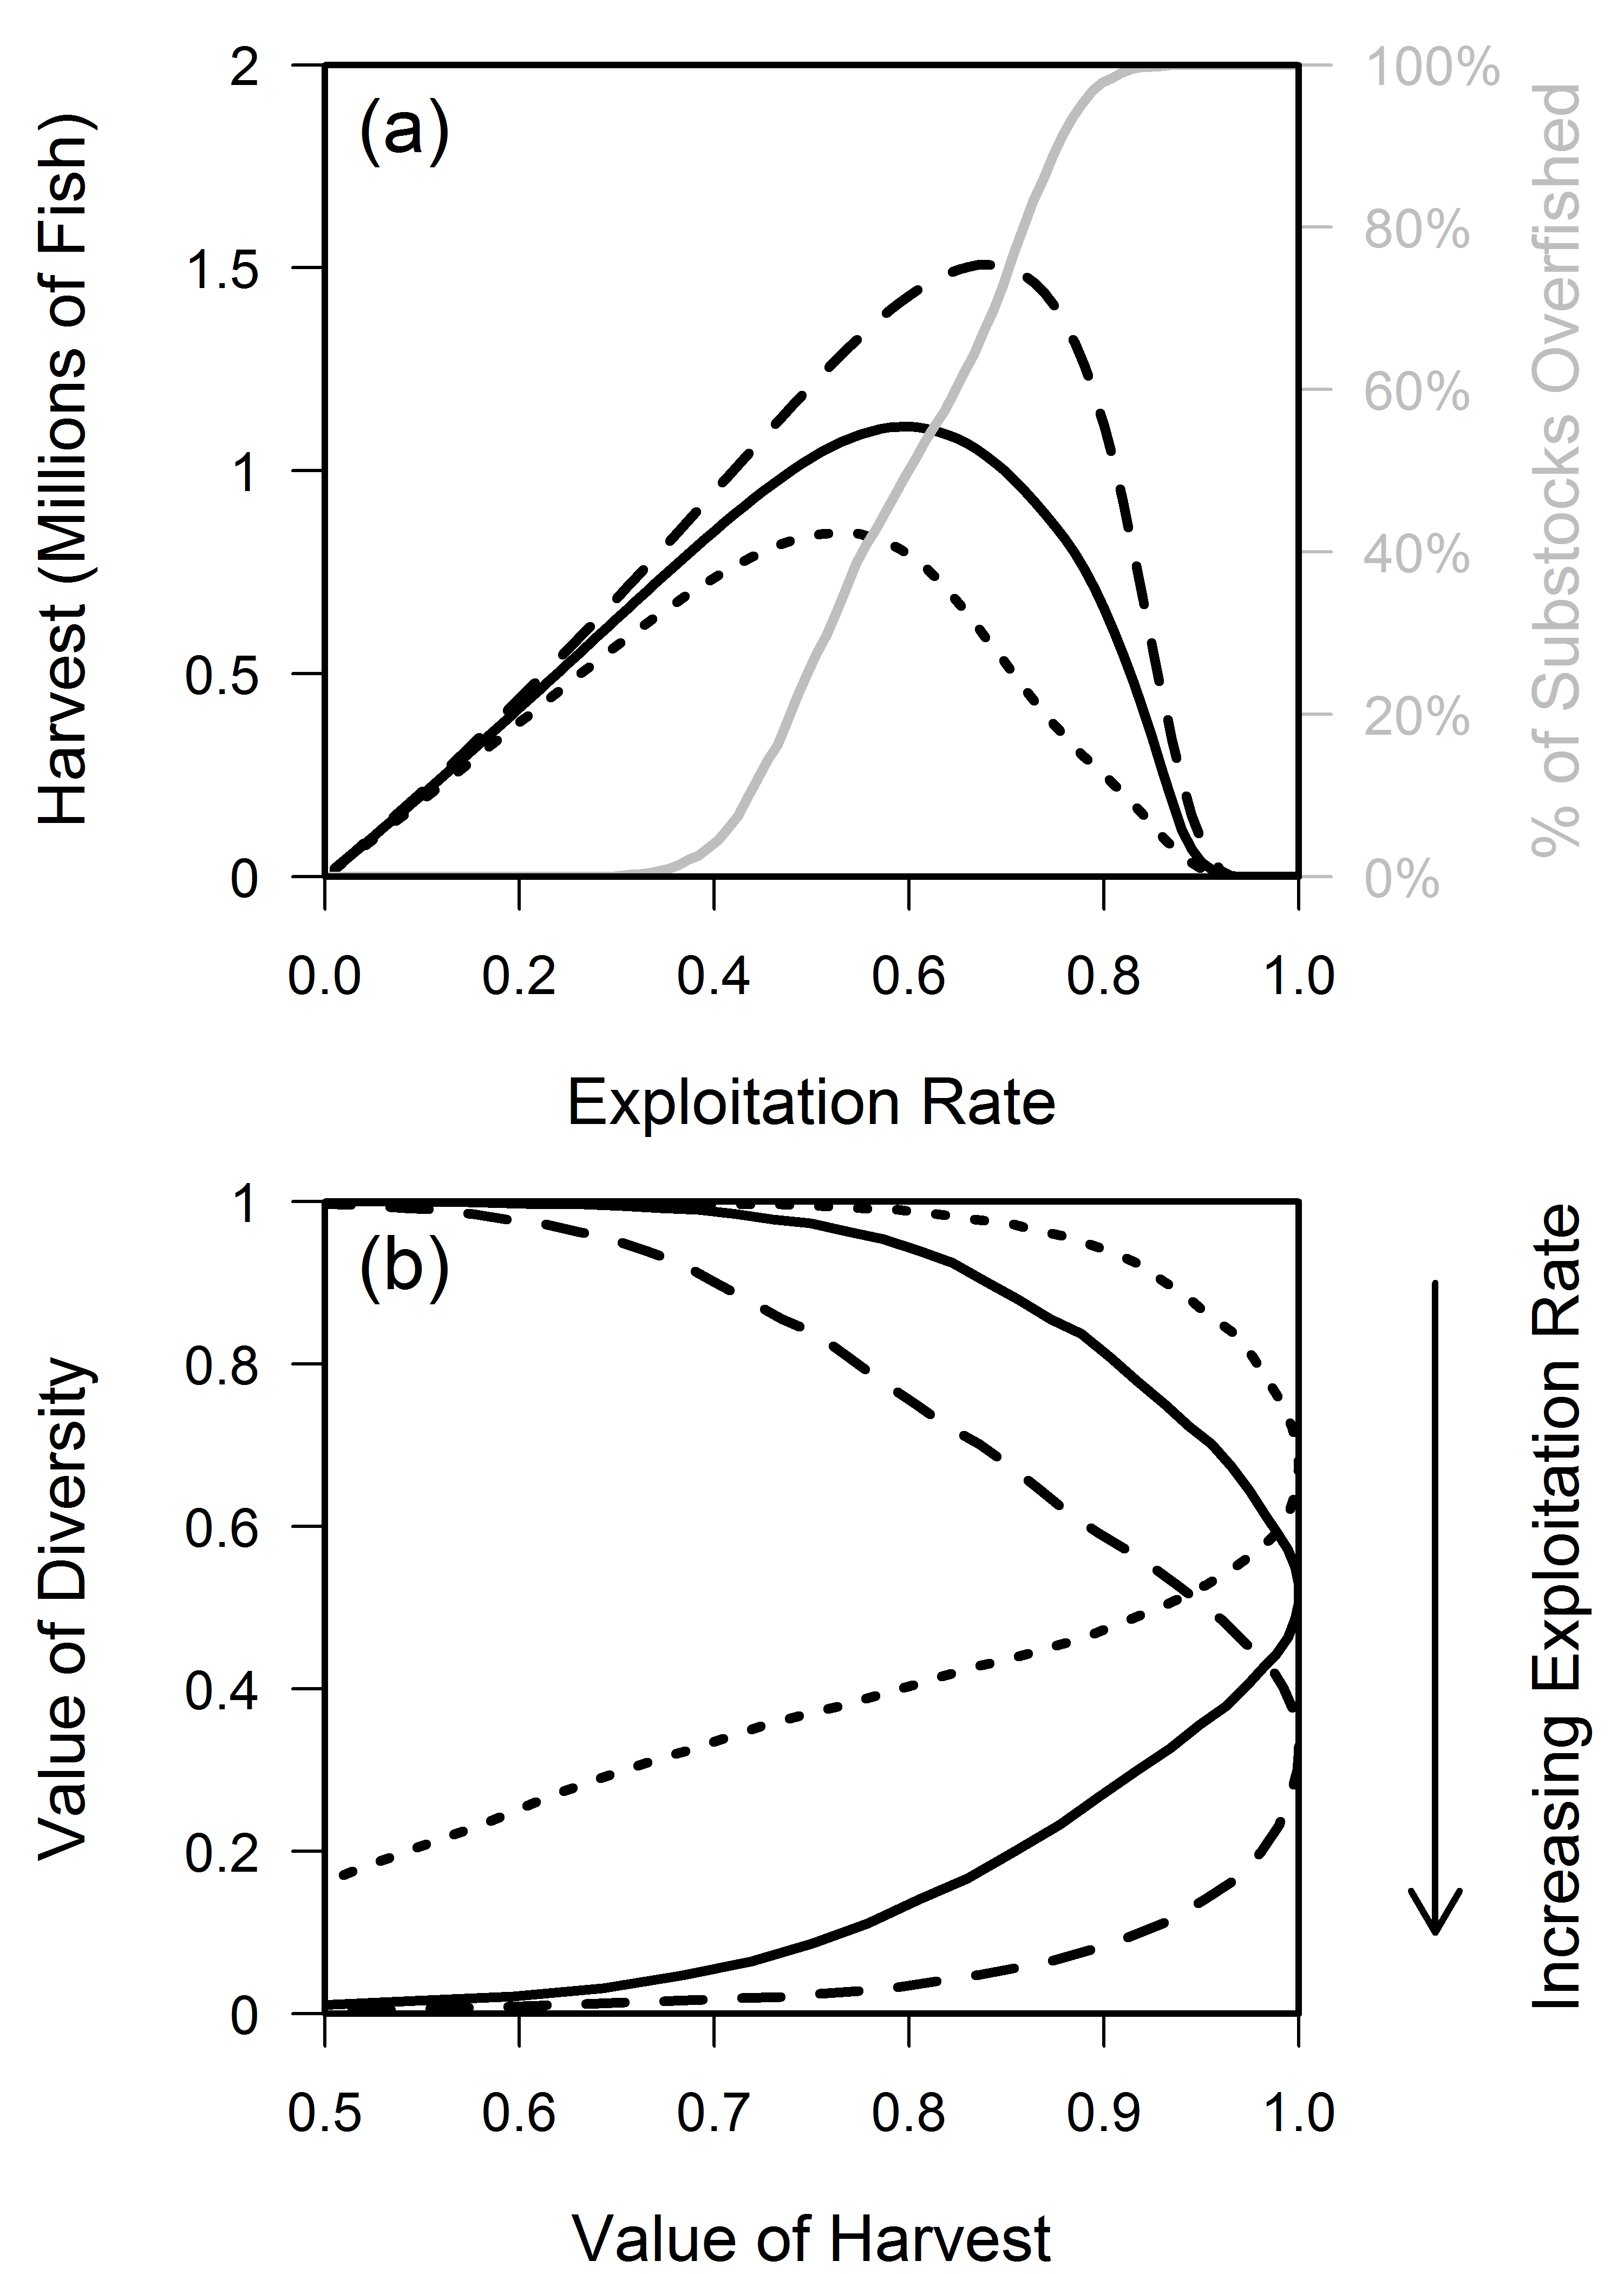
\includegraphics{img/Ch4/trade-off-plot.png}
  \caption{Visualization of how different types of hetergeneity in substock productivity and size influence the shape of trade-offs in mixed-stock salmon fisheries. Solid black likes are the case where stock types are split evenly among large/small and productive/unproductive stocks. Dotted black likes are the case where all small stocks are productive and all large stocks are unproductive, and dashed lines are the opposite (i.e., all big stocks are productive). (\textit{a}) Equilibrium aggregate harvest and proportion of substocks overfished plotted against the exploitation rate (\textit{b}) value of the biodiversity objective (0 = all stocks overfished) plotted against the value of harvest (the long term proportion of the aggregate MSY attained). Notice that when all big stocks are productive (dashed lines), the trade-off is steeper, i.e., more harvest must be sacrificed in order to ensure a greater fraction of substocks are not overfished. }
  \label{fig:trade-off-plot}
\end{figure}

\clearpage

\begin{figure}
  \centering
  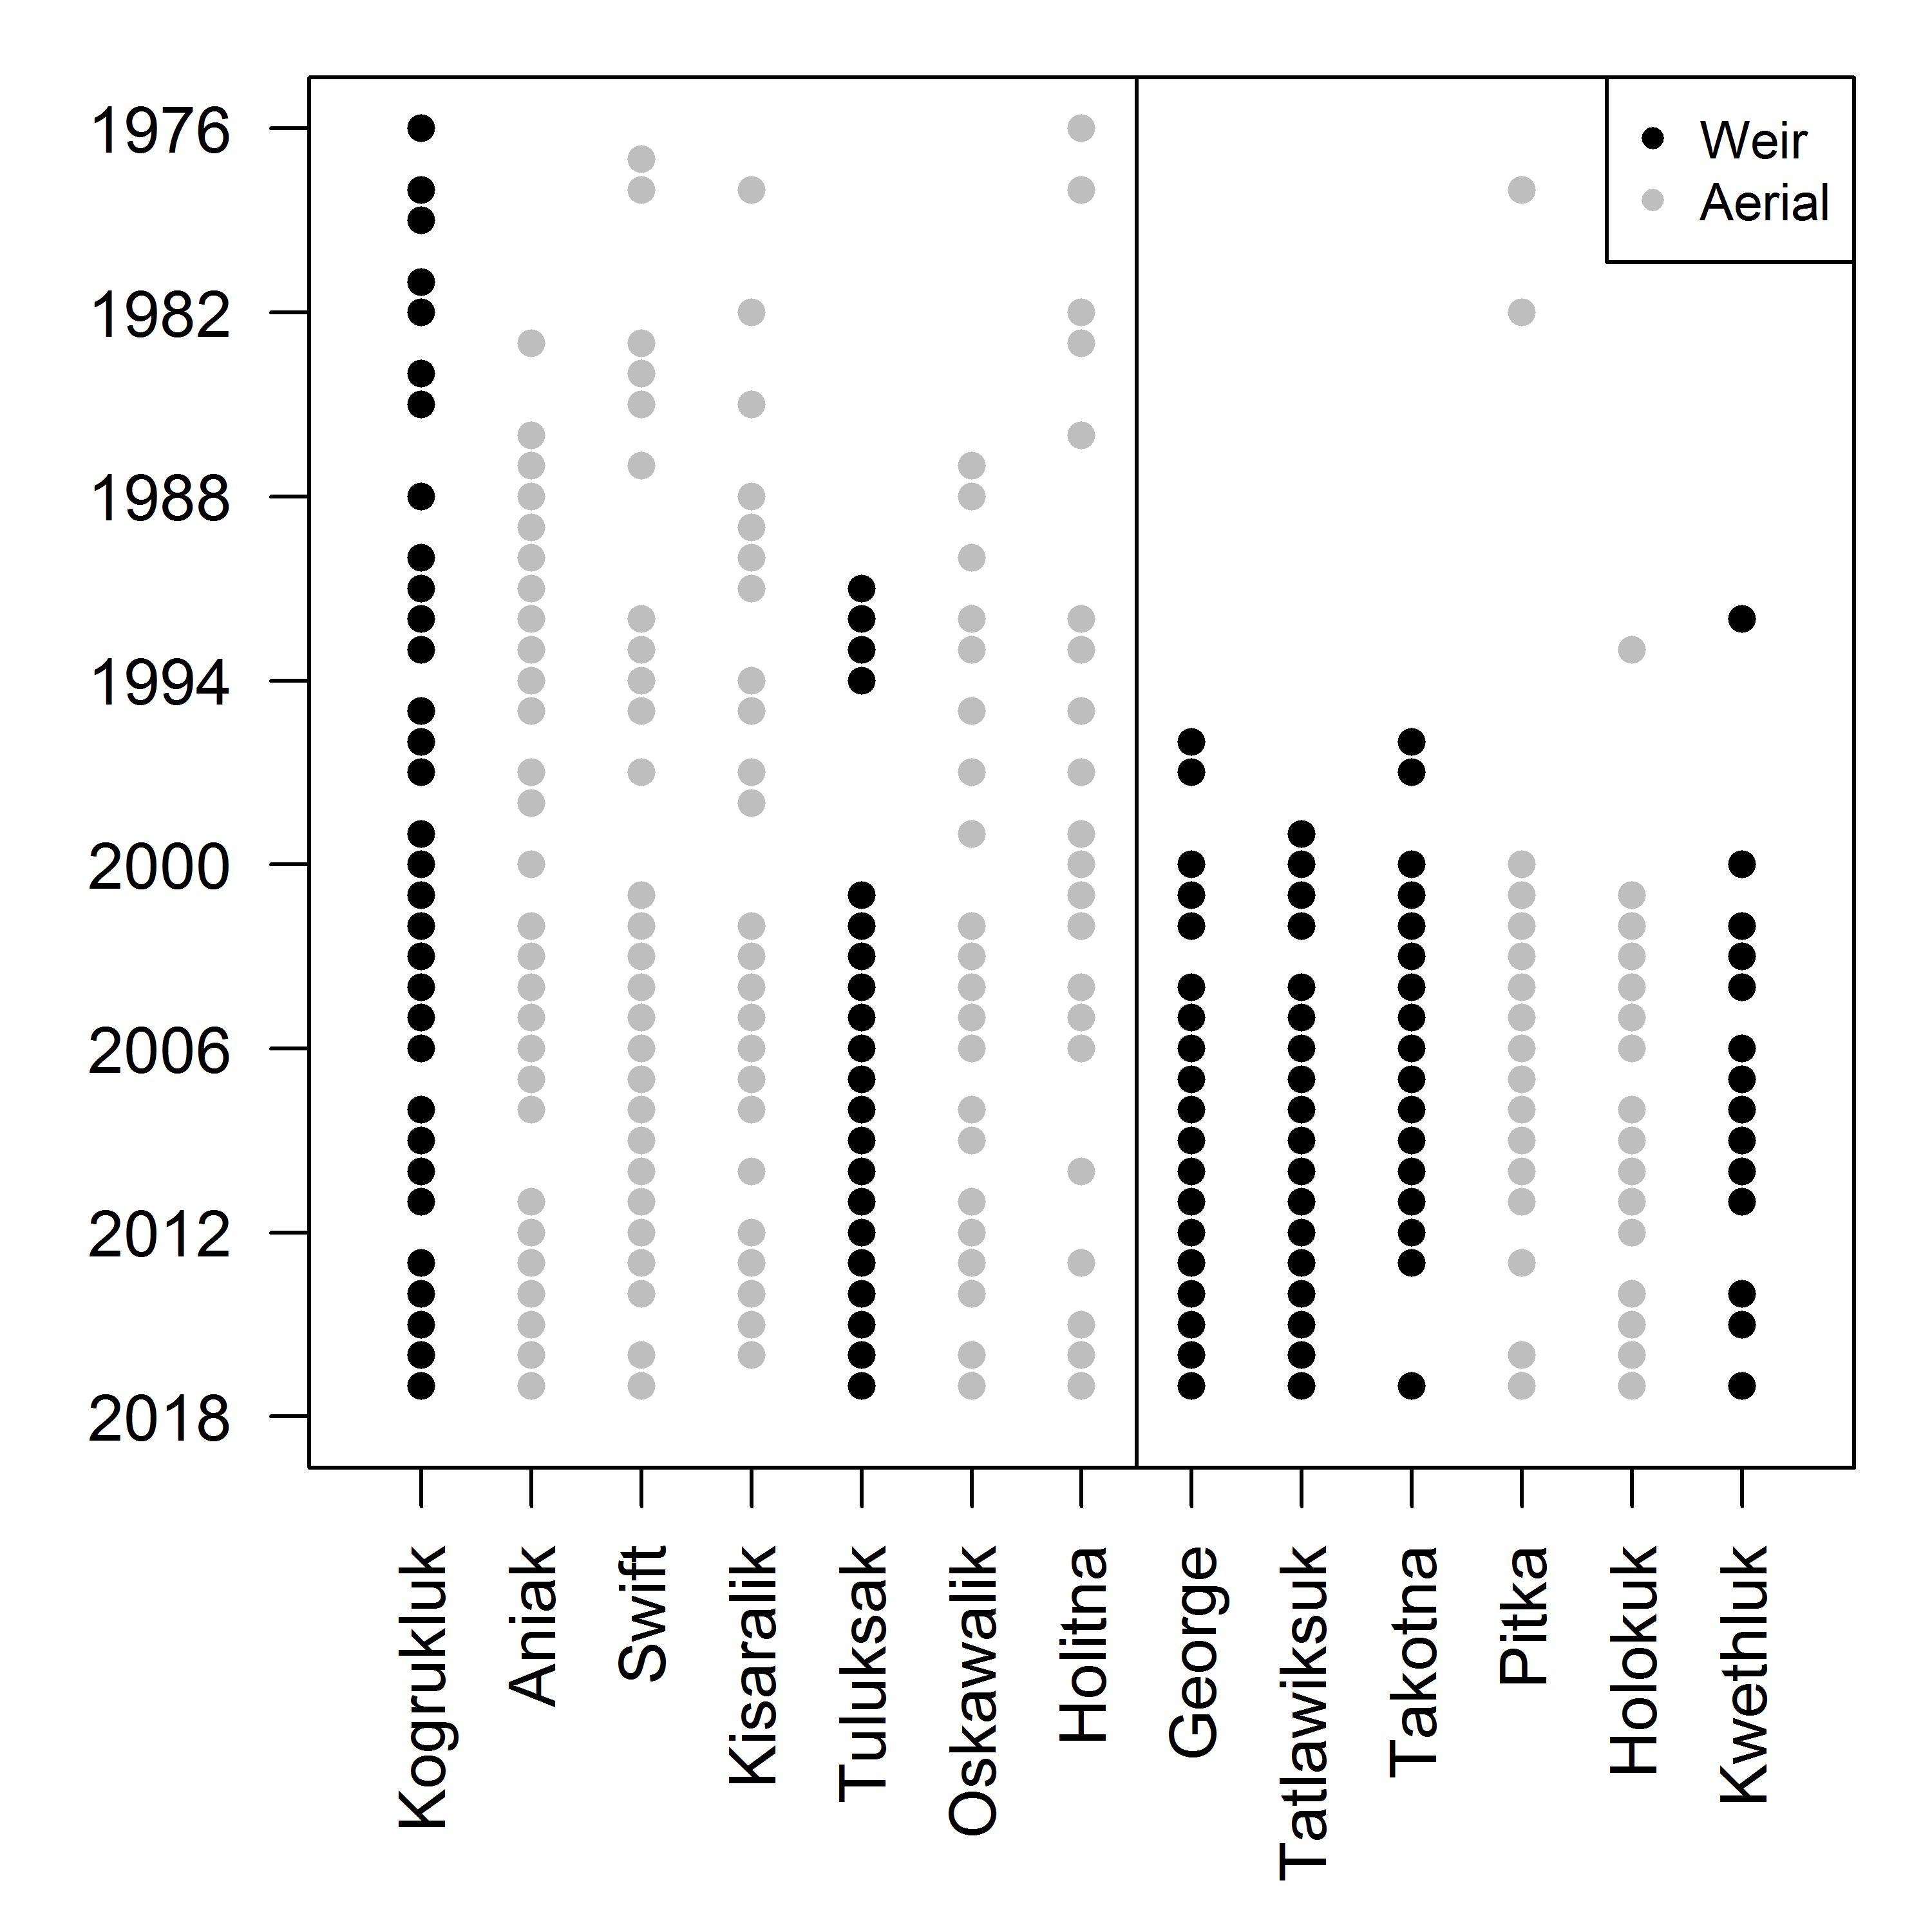
\includegraphics{img/Ch4/obs-freq.jpg}
  \caption{The frequency of escapement sampling for each substock sampled in the Kuskokwim River. Black points indicate years that were sampled for substocks monitored with a weir and grey points indicate years sampled for substocks monitored with aerial surveys. The vertical black line shows a break where > 50\% of the years were monitored for a stock.}
  \label{fig:obs-freq}
\end{figure}

\chapter{Conclusions}\label{ch5}

This chapter contains my thoughts on the topic of the dissertation. What
was found, what will be useful to use in the future, what should be
looked at in more detail?

\setlength{\parskip}{6pt plus 2pt minus 1pt}

\bibliography{cites-without-doi.bib,cites-with-doi.bib}


\end{document}
